\documentclass{article}
\usepackage{graphicx}
\usepackage{amsmath}
\usepackage{amssymb}
\usepackage{float}
\usepackage{CJK}
\usepackage{CJKutf8}
\usepackage{hyperref}
\usepackage{subcaption}
\usepackage{listings}
\usepackage{xcolor}
\lstset{
    backgroundcolor=\color{black},
    basicstyle=\ttfamily\small\color{white},
    keywordstyle=\color{cyan},
    commentstyle=\color{gray},
    stringstyle=\color{green!60},
    frame=single,
    rulecolor=\color{gray}
}
\bibliographystyle{unsrt}
\hypersetup{hidelinks}
\newcommand{\U}{\begin{CJK}{UTF8}{min}ウ\end{CJK}}
\newcommand{\UU}{\begin{CJK}{UTF8}{min}う\end{CJK}}
\newcommand{\OO}{\begin{CJK}{UTF8}{min}オ\end{CJK}}
\newcommand{\UUU}{\begin{CJK}{UTF8}{min}宇\end{CJK}}
\newcommand{\Z}{\begin{CJK}{UTF8}{min}宙\end{CJK}}
\title{New nonstandard analysis and division by zero}
\author{Emmett Lane}
\date{March 2026}

\begin{document}
\setcounter{secnumdepth}{0}
\maketitle
\newpage
\tableofcontents
\newpage


\section{Introduction}

Division by zero is undefined. This is because zero is a multiplicative 
annihilator; every number multiplied by zero yields zero:
\[
0 \cdot x = 0
\]
When we write $a/0 = b$, we are asking for some number $b$ such that 
$b \cdot 0 = a$. But $b \cdot 0$ is always zero, making the equation a 
contradiction for any non-zero $a$. And yet, for mathematicians and 
non-mathematicians alike, the fact that such an elementary operation applied 
to such an elementary number yields something undefined has always been a 
point of fascination. For the most part, despite the incredible advancements 
humanity has made in mathematics throughout history, the best ``solution'' to 
the problem of division by zero has been to simply leave it undefined. 
Anticlimactic perhaps; but it is the most consistent answer mathematics has 
been able to give.\\Or at least, partially. Mathematics has not entirely ignored this problem. 
Calculus, for example, is perhaps the closest it has come to confronting division by zero 
directly, as the concept of the \textit{limit} is the tool which brings us 
infinitesimally close to it without ever actually reaching it. The derivative, 
for instance, is defined as:
\[
f'(x) = \lim_{h \to 0} \frac{f(x+h) - f(x)}{h}
\]
In which we take the \textit{limit} as $h$ approaches, but never reaches, 
zero. This limit describes a \textit{tendency}: what the expression 
\textit{approaches} as $h$ gets arbitrarily small, never actually evaluating 
at $h = 0$, because doing so would yield $\frac{0}{0}$: undefined. The limit 
is, in a sense, mathematics carefully stepping around division by zero without 
ever confronting it directly.\\\\This paper asks a simple question: what if we stopped stepping around it?\\What if, instead of letting $h$ merely \textit{approach} zero, we allowed it 
to \textit{reach} zero by \textit{fundamentally} reconsidering what zero is 
and what it means for a quantity to \textit{be} zero? This proposition may 
seem unorthodox by conventional mathematical standards; yet it is one which 
I chose to explore. From this exploration emerged a new framework along with 
a corresponding number system: the \textit{absolute hyper-reals}. This paper 
is devoted to motivating and constructing this number system, describing the 
philosophical and structural ideas which underpin it, and ultimately defining 
division by zero through it.

\newpage\section*{Abstract}
This paper develops a speculative number system called the \emph{absolute 
hyper-reals}, built on a single philosophical departure from standard 
mathematics: that magnitude is \textit{discrete} at extreme scales rather than always remaining continuous. A 
fundamental lower bound of non-zero magnitude is postulated: the 
\emph{absolute infinitesimal} $\varepsilon_\Omega$, below which all 
quantities are considered \textbf{zero-equivalent}. Its reciprocal, the 
\emph{absolute hyperfinite} $\omega_\Omega$, forms the corresponding upper 
bound - serving as the \textbf{largest} possible \textit{finite} number.\\\\ From this the standard notion of 
continuity is replaced by \textit{mathematical data}: where magnitude 
fails, data takes hold. Zero is no longer merely a boundary that sequences 
approach; it is a number that can be reached and reasoned about. Division by zero, rather than being undefined, acquires a precise geometric 
meaning: in this theory, a circle is defined as two simultaneous entities. 
Physically, it is a discrete polygon whose edges are as small as the number 
system permits. Virtually, it is a regular polygon of side length $0$ and 
side count $\frac{C}{0}$, and it is this virtual definition which defines 
curvature, and gives division by zero its meaning.
\\From this foundation, the fundamental concepts of calculus, such as limits, 
derivatives, and integrals, are reinterpreted within the absolute 
hyper-reals, forming the basis of what I call ``new'' nonstandard analysis.
\newpage
\section{Chapter 1 - Metaphysics and Mathematical Data}

In mathematics, nothingness is flattened into a single, uniform concept: zero. To say that we have zero of something, for example, zero meters, zero apples, or zero seconds, is, mathematically speaking, to say the same thing in every case because the particular kind of thing we have disappears. \\This is because zero has an annihilator property, in which everything multiplied by zero returns zero, which makes it so nothingness cannot be accumulated or differentiated in the way that “somethings” can. Two nothings are not more than one nothing; three nothings are not different from none at all. Once quantity collapses into absence, counting loses its meaning. It is why: $$0\cdot \text{meters}=0\cdot \text{seconds} = 0\cdot \text{apples} = 0 \cdot2=0\cdot3=0$$Because multiplication by zero erases all distinctions. Whatever was there, units, magnitude, or kind - is reduced to the same mathematical descriptor: zero. And in reality as well, we can ascertain this to be the case - zero apples is nothingness, zero meters is also nothingness, and because nothingness has no physical discernible features, it is all one thing - it is all zero, it is all \textbf{nothing}.\\\\ And yet, if we were to consider and approach this from a philosophical angle, particularly a metaphysical or ontological angle, the notion of nothingness becomes far less straightforward. We ask ourselves: what is nothing? What does it mean to be nothing? Is there such a thing as ``different'' nothings? Is there a point in which something ceases to be able to be considered something, and it becomes nothing? And if this point does exist, is this nothing which was attained from this previous something the same as a nothing that never was?\\Well, in reality, these questions resist definitive answers. These are, after all, metaphysical questions, and there is no clear-cut method for arriving at definitive answers; at most, one can only reflect upon them.\\ However, in mathematics, these metaphysical questions do not seriously arise, and for good reason. Once quantity vanishes, the particular nature of what is being measured becomes irrelevant, and treating zero things as being different to zero other things serves no computational purpose. Moreover, because of the continuous nature of number systems, there is no sharp boundary between a nonzero magnitude and zero itself. Asking where nothing “begins” is therefore largely meaningless in a mathematical context. Instead, mathematics describes a \textit{limit}, which describes a tendency toward a value without requiring that the value itself be reached or reified as a physical boundary. \\ And yet, one might ask: what if it were not so simple? What if we attempted to integrate these philosophical notions of nothingness into the concept of zero itself, thereby reinventing the number entirely? What if different forms of nothingness were acknowledged, or if a hard boundary existed: one in which the point being evaluated is not merely approached, but actually crossed? \\ What would emerge would be a whole new way of imagining numbers and continuity: and this new concept in which we integrate these absurd philosophical queries into mathematics is what I call ``\textbf{mathematical data}''. 

\subsection{Actuality and Virtuality}To understand mathematical data \footnote{technically speaking, a more accurate label than mathematical data would be mathematical \textit{metadata}, however, that is a bit too long, so mathematical \textit{data} is preferred}, even though it really \textit{is} just metadata about numbers as a whole, and its role in this theory, one must first accept that the concept of a number is philosophically reconceived here. Instead of numbers being abstract representations of quantity, they are described in two parts: ``actuality'' (also called \textit{actual value}) and ``virtuality'' (also known as \textit{virtual data}).
Actuality is understood as the \textit{quantity} of a number as an abstraction, it is the ``how much'' of a number. This is not a foreign concept, because traditional notions of numbers consider only their actuality. When we describe the number one, we fundamentally understand it as being a \textit{quantity} of one, and this is its actuality. Essentially, what a number's value is \textbf{is} its actuality.
What makes numbers in this number system different, however, is that they comprise another aspect, one which traditional mathematics doesn't consider. This other aspect, which \textit{mathematical data} describes, is called the \textit{virtuality} of a number (we also say \textit{data}, \textit{virtual value}, or \textit{virtual information} depending on context). Virtuality and mathematical data describe the same idea and concept: namely, \textit{information} about a number \textit{beyond} its actuality. Specifically, virtuality (and data as a whole) is defined as ``metadata'' or ``information'' about numbers. Data can be thought of as a \textit{qualitative} framework describing information about a number: its origins, what it is a result of, its context, and other trivial and non-trivial information. Data is perhaps best understood as an identification card or ``passport'' for numbers.\\ Utilizing virtuality and actuality, if we consider  the number ``4'' in this number system, we would say it has an actuality (actual value) of 4 - (it is literally 4 units) but a virtuality (mathematical data) of being created by me, just now, for the purpose of demonstration. This virtuality aspect of a number is very much based upon metaphysics and ontology, because this trivial, and even sometimes ``unknowable'' information about a number being carried as some sort of ``essence'' is what virtuality describes.\\
A simple way to see this is by the following:$$1=1+\text{data}$$ $$1=1+0$$ In which the left hand side has the number 1 as a whole, and the right hand side illustrates the number's actuality (quantity of 1) plus its virtuality (information which does not contain value). To demonstrate actuality and virtuality, we shall consider a very simple following real-world example of comparing two distinct objects, applying certain metaphysical concepts, and then describing the numbers through their actuality and virtuality.
\subsection{Different Absences}For our example, we can consider having an apple and a banana. Now, in their presence, they are different objects, as we can touch, feel, and taste the difference between the two, because in our reality, the matter which composes one differs from the matter which composes the other. However, in their absence, they no longer possess the physical features to distinguish each other - zero apples is zero bananas.\\ But, when considering this on an \textit{ontological} level, the essence of their absence is not identical. Despite their physical indiscernibility, the absence of apples is not the same as the absence of bananas on a deeper, metaphysical level. This view holds that the concept of ``absence'' is not merely a void but is tied to the nature of the objects that are absent. The absence of apples might carry a different essence than the absence of bananas, even if, in practice, both are described as zero objects. In this context, the metaphysical interpretation would suggest that these two ``nothings'' are not equivalent because the objects they refer to, apples and bananas are distinct at an ontological level, and their absence must therefore be treated as distinct as well, which is what \textit{mathematical data} does. Describing the apples and bananas with their actuality and virtuality, we say that although an apple is \textit{not} a banana, in their absence, $0\cdot apples=0\cdot bananas$ is true because the actuality of zero apples is the same as the actuality of zero bananas, because $0=0$. However, we can interpret that the metaphysical essence of being an apple is preserved \textit{virtually}, making it so these two zeroes have a different ``virtuality''. We denote this using the subscript \textit{v} (with the subscript \textit{v} meaning \textit{virtuality)}, attached to an equal sign (or a is not equal sign) on either side of the equation, to illustrate an actual equivalence but a virtual difference. For this example, since the absence of apples and bananas are metaphysically distinct, we illustrate the following actual equality and a virtual inequality: 
$$0\cdot \text{apples}=0\cdot \text{bananas}$$ $$0\cdot \text{apples} \ _v{\neq}{}_v \ 0\cdot \text{bananas}$$  we use $_v{\neq}{}_v$, to indicate that both zeroes have the same actual value (of zero) but virtually represent different objects.\\\\On the surface, the invention of \emph{mathematical data} may seem trivial or even unnecessary. Why does it ``matter''? Why invent it at all? The truth is, for traditional number systems, mathematical data is indeed superfluous. However, in this newly invented number system, the \emph{absolute hyper-reals}, mathematical data is not only integral, but indispensable. The system relies heavily on it, and the ability to store qualitative information about numbers becomes essential for reinterpreting and re-imagining concepts like continuity. In this context, data is not just an addition; it forms a core aspect of this new number system itself.
\newpage
\section{Chapter 2 - Introduction to the Absolute Hyper-Reals}

\subsection{The Hyper-Reals}
Nonstandard analysis, originally developed by Abraham Robinson, extends the real number line to include infinitesimals (denoted by $\varepsilon$) and infinite quantities (denoted by $\omega$). Infinitesimals are nonzero quantities smaller in magnitude than every real number, while infinite values are quantities larger than every real number but are not ``infinity'' in the sense that they are not invariant under finite arithmetic operations. For example, an infinite quantity $\omega$ is distinct from $\omega + 1$, with $\omega + 1 > \omega$, unlike the formal symbol $\infty$, for which $\infty + 1$ and $\infty$ are not regarded as distinct magnitudes. In this sense, the hyper-reals are \emph{non-Archimedean}, as unlike the real numbers, they do not satisfy the Archimedean property, as there exist positive infinitesimals $\varepsilon$ such that no finite real multiple $n\varepsilon$ (for any $n \in \mathbb{N}$) exceeds a given real number, and dually there exist infinite elements $\omega$ that dominate all real numbers, allowing a precise distinction between finite, infinitesimal, and infinite magnitudes \cite{ponstein}.
$$\varepsilon<\mathbb{R^+}$$ $$\varepsilon>0$$$$\omega>\mathbb{R^+}$$ $$\omega\neq\infty$$This extension allows concepts such as limits, continuity, and differentiation and integration to be reformulated using infinitesimals rather than traditional $\varepsilon$--$\delta$ arguments, thereby more closely resembling the original formulations of calculus introduced by Leibniz (through differentials) and Newton (through fluxions).
\\Inspired by this number system, this paper introduces a new number system, referred to as the \emph{absolute hyper-real numbers}. This system is conceptually similar to the hyper-real numbers and shares many of the same foundational ideas: both were developed with the goal of reformulating calculus through a reexamination of concepts such as limits and continuity, achieved by the admission of infinitesimal and infinite quantities. Despite these similarities, there is a fundamental conceptual distinction between the hyper-reals and the number system introduced here. In a manner, it is a simple distinction, yet it is this difference which completely reformulates and re-interprets \textit{continuity}. You see, like most real-derived number systems, the hyper-reals are classically understood to be \textbf{absolutely continuous}: meaning that although they extend the real numbers to include infinitely small and infinitely large values, they do not contain a ``smallest'' nonzero element and no ``largest'' element. As a result of this, infinitesimals - which are described as being infinitely small, \textit{can} be subdivided indefinitely without collapsing to zero, all while still retaining nonzero magnitude. Although they would be meaninglessly small, higher powers of an infinitesimal, such as its square or cube, would still technically remain greater than zero. We illustrate this below by presenting a real number line alongside hyper-real infinitesimal monads (where a monad denotes the set of values infinitesimally close to a given value \cite{numberphile_monad}), with each monad corresponding to higher powers of infinitesimals. 

\begin{figure}[H]
    \centering
    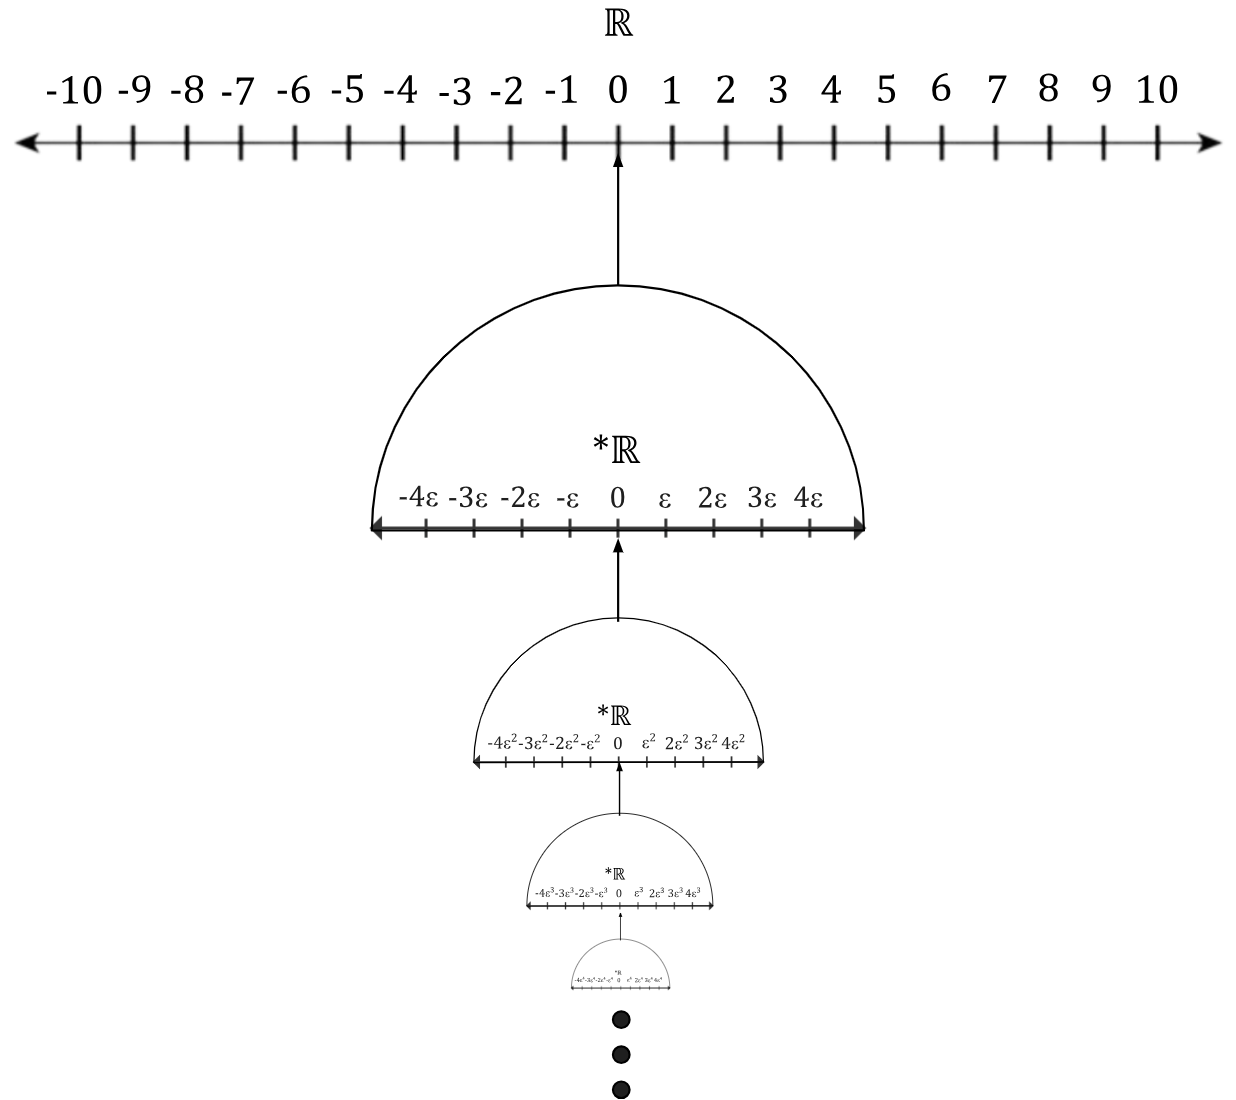
\includegraphics[width=1\linewidth]{Screenshot 2025-12-23 at 15.55.00.png}
    \caption{Real line and infinitesimal monads of higher powers}
    \label{fig:placeholder}
\end{figure} This process of dividing and shrinking the magnitude of infinitesimals is, in principle, unending - one can produce infinitesimals of progressively smaller orders indefinitely because the hyper-real number line is absolutely continuous, and no obstruction exists to prevent the existence of ever-smaller infinitesimals. In essence, there is no theoretical limit to how small an infinitesimal can become within the hyper-real number system, and despite how close one gets to zero, zero is never reached. But what if there was? What if, contrary to standard number line convention, this infinite descent into smaller infinitesimals were to terminate after some possible hyper-real infinite iteration? What if there existed a smallest positive infinitesimal, a fundamental lower bound to how small a quantity could be, where any smaller would simply collapse to zero, and what would that entail?
Conventional wisdom and classical analysis hold that such a minimal infinitesimal cannot exist, for its presence would contradict the inherent nature of the continuum as an infinitely divisible entity. In both the hyper-real system and other real-derived number systems, one should always be able to “zoom in” infinitely without ever arriving at a smallest scale or “atomic” monad. The continuum, by definition, resists such discretizations. 
\subsection{The Absolute Hyper-Reals} It  is precisely where our number system - the \textit{absolute hyper reals}, comes into play, as it is here where we propose a number system in which there \textbf{does} exist a smallest element (alongside a smallest monad), thereby interpreting the number line as not being an infinitely divisible entity. This assumption gives rise to the \textit{absolute hyper-real} number line, which departs from conventional number systems and offers an alternative approach to the treatment of infinitesimals and infinities, and, most importantly, to the notion of \emph{continuity} as a whole.\\ We represent the set of all absolute hyper-real numbers using a new set symbol $\mathbb{R}_\Omega$, distinct from the hyper-real ${}^\ast\mathbb{R}$. The inspiration behind the usage of a capital omega subscript ($\Omega$) instead of using an asterisk like the hyper-reals comes from the notion of absolute infinity in set theory \cite{wiki_absolute_infinite}. \\ The absolute hyper-real number line is founded on the same ideas and principles as the \textit{hyper-real} number line - both are described as being extensions of the reals designed to include infinitesimal and infinite values, thereby superseding the real numbers. However, the key point at which this system deviates from the hyper-reals, and from conventional number lines more generally: is that it is a \textbf{bounded} number system, in which there exist minimal and maximal nonzero and non-infinite magnitudes. This is quite striking, because although the real number system is unbounded and contains no ``smallest and largest'' elements, the absolute hyper-real number system, which serves as an extension of the reals suddenly \textit{does} include these absurd elements.\\At first glance, this may seem absurd: how can a supposedly unbounded extension of the reals suddenly possess bounds? This is not merely paradoxical in appearance, it is paradoxical in essence, and intentionally so. The contradiction is the foundation of this system. The main idea is that these bounds are never encountered \textit{within} the real numbers themselves; they arise only when one ventures \textit{outside} $\mathbb{R}$ and into the absolute hyper-reals. Since $\mathbb{R}$ is conceptually embedded within the absolute hyper-reals, the number line behaves classically and continuously as long as we remain within the reals. Beyond them, however, the continuum begins to break down: the number line deviates from standard behavior by functioning \textit{discretely} at very small scales and failing to extend beyond very large scales, because \textbf{actuality collapses beyond these bounds}. This strange phenomenon is caused by ``\textit{absolute}'' elements, so named because they represent the extreme limits of magnitude itself. The first such number is the \emph{absolute infinitesimal}, denoted by $\varepsilon_\Omega$, and the second, which is its reciprocal, is the \emph{absolute hyperfinite}, denoted by $\omega_\Omega$. In this work, the term \emph{hyperfinite} is preferred over \emph{infinite}, since infinity itself exists as a separate entity from the hyperfinites in this theory.
\subsection{The Absolute Infinitesimal}We define the absolute infinitesimal in a manner similar to a hyper-real infinitesimal: it is a number whose magnitude is smaller than all real numbers but strictly greater than zero. However, this model further extends the definition by treating the absolute infinitesimal as being \textit{absolutely} infinitesimal, meaning it is infinitesimal to every standard magnitude, making it a nonzero, strict lower bound of magnitude, meaning that no number exists that is smaller than it yet greater than zero. We define the absolute infinitesimal as follows\footnote{This definition is also called the ``simple lower bound'' of $\mathbb{R}_\Omega$}: 
  $$\varepsilon_\Omega \in \mathbb{R}_\Omega, \quad \varepsilon_\Omega \neq 0, \quad \varepsilon_\Omega < \mathbb{R}^+$$
This gives rise to the lower bound property: any value of magnitude less than $\varepsilon_\Omega$ is zero-equivalent:
$$0 \leq |x| < \varepsilon_\Omega \implies x = 0$$
Consequently, for $n, k \in \mathbb{R}_\Omega$:
$$|n| < 1 \implies n \cdot \varepsilon_\Omega = 0$$
$$|k| \geq 1 \implies |k \cdot \varepsilon_\Omega| > 0$$Consequently, the number line in which absolute infinitesimals appear no longer functions as continuous. Instead, since the absolute infinitesimal is the smallest possible non-zero value, it operates discretely at this level: values can increase only by one absolute infinitesimal unit, the smallest possible nonzero magnitude increase. As a result, only integer multiples of the absolute infinitesimal exist, with no values in between. The following image visualizes the absolute hyper-real line at the absolute infinitesimal level, illustrating the monad below the reals, which is the absolute infinitesimal monad. Since absolute infinitesimals are the absolute smallest, the number line must be stretched to observe them, making them appear as discrete dots. These absolute infinitesimal points collapse to form a singular continuous line.

\begin{figure}[H]
    \centering
    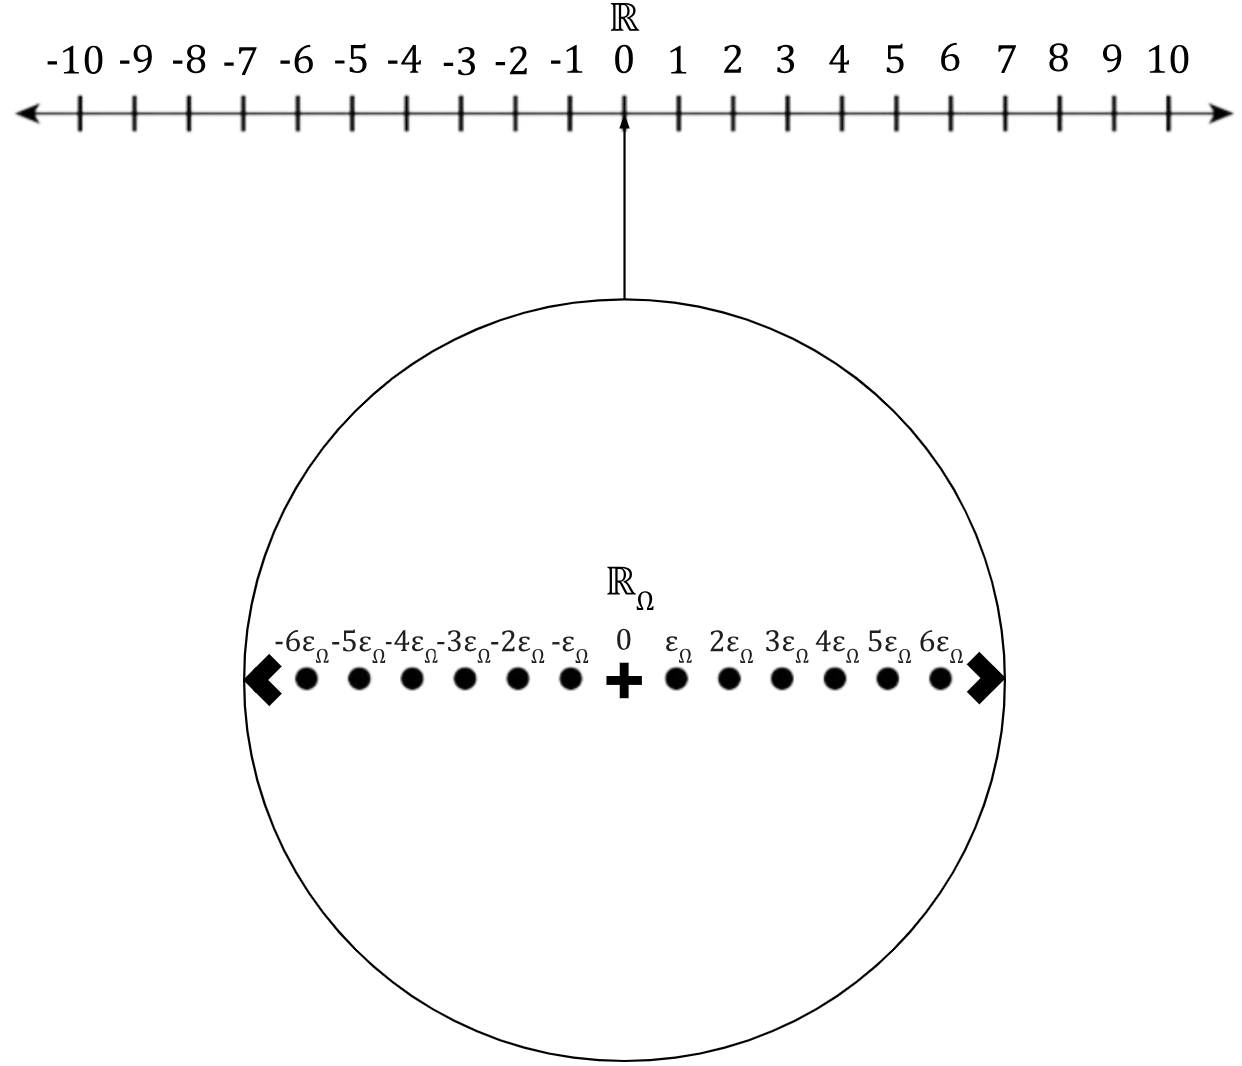
\includegraphics[width=1\linewidth]{Screenshot 2025-12-23 at 23.37.59.png}
    \caption{Discrete absolute infinitesimal monad within the Reals}
    \label{fig:placeholder}
\end{figure}

\subsection{The Absolute Hyperfinite}
The absolute hyperfinite is defined as the reciprocal identity of the absolute infinitesimal $\frac{1}{\varepsilon_\Omega}=\omega_\Omega$ , and it is defined in a manner similar to its hyper-real analogue, being larger than all real numbers, but is not ``infinity''. However, this number system bears a far more \textbf{bold} definition of having the absolute hyperfinite be defined as being the hard upper limit for “finite” magnitude, because again, it is ``\textit{absolutely}'' hyperfinite, meaning no larger \textit{finite} number than it exists, and instead, this theory interprets that infinity is reached. We define the absolute hyperfinite $\omega_\Omega$ as follows\footnote{This definition is also called the ``simple upper bound'' of $\mathbb{R}_\Omega$}:
$$\omega_\Omega \in \mathbb{R}_\Omega, \quad \omega_\Omega \neq \infty, \quad \omega_\Omega > \mathbb{R}^+$$
This gives rise to the upper bound property: any value of magnitude greater than $\omega_\Omega$ is infinite, and infinity is not an element of $\mathbb{R}_\Omega$:
$$\infty \notin \mathbb{R}_\Omega$$
Consequently, for $n, k \in \mathbb{R}_\Omega$:
$$|n| \leq 1 \implies n \cdot \omega_\Omega \in \mathbb{R}_\Omega$$
$$|k| > 1 \implies k \cdot \omega_\Omega = \infty$$
This makes the absolute hyperfinite the largest finite quantity within this number system - serving as its upper bound. In the absolute hyper-reals, any increase beyond this magnitude essentially renders the concept of actuality asunder, and \textit{infinity} is therefore reached. Just as the absolute infinitesimal is in a way the ``barrier'' between magnitude (actuality) and zero, the absolute hyperfinite is the ``barrier'' between magnitude and \textit{infinity}. Naturally, this also means that infinity itself is substantially reinterpreted in this system and differs markedly from conventional notions. Although this interpretation will be examined in detail in a later chapter, this brief discussion is necessary, as the absolute hyperfinite cannot be meaningfully understood without reference to the system's conception of infinity. \\
The first concept to understand about infinity in this theory is that it is an ``entity'' separate from the set of values comprising the absolute hyper-reals. Infinity is defined as \textit{not} being an element of the absolute hyper-real set, $\mathbb{R}_\Omega$, but instead as something outside of it. This is because conceptually, the absolute hyper-reals consist only of \textbf{finite} values: values that lie along the absolute hyper-real number line, extending from $-\omega_\Omega$ to $\omega_\Omega$, where $|\omega_\Omega|$ represents the largest possible finite magnitude. Numbers \textit{larger} than $|\omega_\Omega|$ are therefore considered infinite, and these resulting numbers are therefore ``part'' of infinity. Therefore, infinity comprises all the ``elements'' that $\mathbb{R}_\Omega$ does \textbf{not} contain. In this number system, infinity is therefore redefined by a change in what it means to be \textit{finite}. Here, ``finite'' is taken to mean \textbf{belonging to the absolute hyper-real set} $\mathbb{R}_\Omega$. Any quantity that does not belong to this set is, by definition, classified as infinite. One consequence of this definition is that expressions which would traditionally be regarded as finite, such as $2\omega_\Omega$, are instead labeled infinite, even though there is nothing intrinsically ``infinite'' about them in the usual sense. This raises an obvious question: how can a quantity be called infinite if it is not truly infinite? The answer lies in a conceptual distinction. In this theory, actuality is taken to collapse beyond the absolute hyperfinite - which means that values larger than the absolute hyperfinite do not really exist as \textit{standalone} actual values. This makes infinity as a whole not traditionally a point, a direction, or a continuation of the number line, but something \textit{entirely} different. Infinity is imagined as a \textit{space} in which actuality and value itself breaks down. Unlike the real numbers, which are arranged along a line with a meaningful notion of order and magnitude, infinity represents a domain where magnitude, size, order, and comparison no longer apply. Within infinity there is no ``larger'' or ``smaller''; it is a homogenized domain encompassing everything beyond the hyperfinite. Accordingly, infinity is not defined as the ``next value'' after the hyperfinite, but as a separate kind of mathematical object altogether. It is better understood through what we call \textit{virtuality}, which we refer to as \textbf{specific infinite data} in this case. Returning to the example of $2\omega_\Omega$, this quantity is interpreted as a specific infinite data of infinity: it is not a unique actual value and it is not represented as a point on a line, but rather it is represented as belonging to infinity as a whole. \\
\begin{figure}[H]
    \centering
    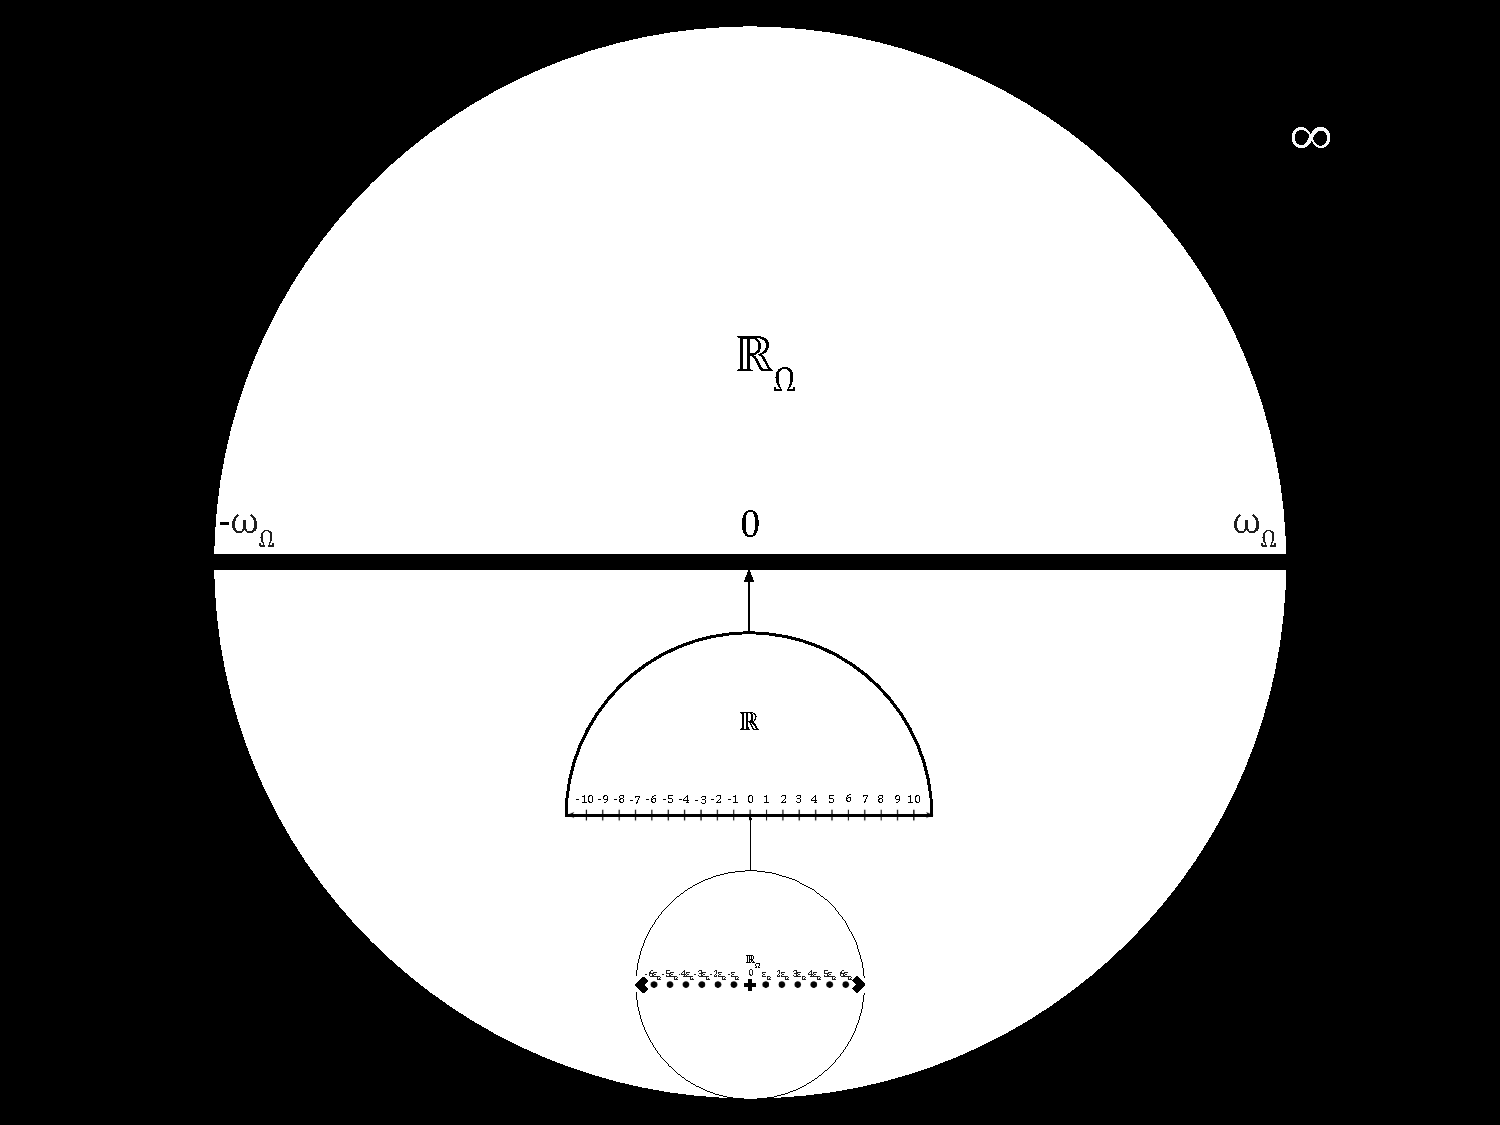
\includegraphics[width=1\linewidth]{Untitled drawing.pdf}
    \caption{The absolute hyper-reals at the absolute hyperfinite scale}
    \label{fig:placeholder}
\end{figure}
Now, this is only the introduction of infinity within this number system - to fully delve and understand infinity requires proper establishment of how virtuality functions, and most importantly, how virtuality keeps this number system in check.
\newpage
\section{Chapter 3 - Algebraic Structure and the Bound Property of $\mathbb{R}_\Omega$}

Having established the foundational concepts of the absolute hyperfinite number system, this chapter explains the basic algebraic properties of $\mathbb{R}_\Omega$, including commutativity, associativity, identities, inverses, and closure, alongside arithmetic operations involving absolute infinitesimals and absolute hyperfinites.\\Before beginning, it should be noted that this chapter discusses algebraic properties purely through \textbf{actuality}, and not \textit{virtuality} - virtuality will be covered in a later chapter. \\For the most part, this number system is built similarly to the reals, asserting that many of the same rules and axioms governing $\mathbb{R}$ transfer to $\mathbb{R}_\Omega$. What this means is that absolute hyper-reals are often treated as if they were real, while accounting for deviations caused by the absolute elements. The primary algebraic irregularities occur when values exceed minimum ($\varepsilon_\Omega$) and maximum ($\omega_\Omega$) thresholds.

\subsection{Structural Relationship to the Reals}

The absolute hyper-reals are conceptually an extension of the real numbers, meaning $\mathbb{R} \subseteq \mathbb{R}_\Omega$. However, this is a somewhat paradoxical assertion, as previously mentioned, the traditional reals extend infinitely and are absolutely continuous, while the absolute hyper-reals only extend to $\pm\omega_\Omega$ and can only be subdivided until $\varepsilon_\Omega$ is reached, effectively ``breaking'' the traditional number line. Our argument is that despite the fact this is the case, the real numbers nest within the absolute hyper-reals as an ``infinitesimal subsection'' where the number line behaves ``normally'': infinitely extending and infinitely sub divisible.

\subsubsection{Why $\mathbb{R}_\Omega$ Is Not a Field}

Although many properties of $\mathbb{R}$ are present in $\mathbb{R}_\Omega$, the system cannot be conventionally described as a field, ring, or group because it is not closed under addition involving $\omega_\Omega$. Since $\omega_\Omega$ represents a boundary between the continuum and infinity ($\infty$), and infinity is not part of the absolute hyper-reals, operations that exceed $\omega_\Omega$ produce results outside $\mathbb{R}_\Omega$. The system is best described as ``field-like'': it is closed under real arithmetic but not under its own arithmetic.

\subsubsection{Standard Algebraic Properties}

Despite not being a field, $\mathbb{R}_\Omega$ possesses the following standard properties:

\textbf{Associativity:} For all $a, b, c \in \mathbb{R}_\Omega$:
\begin{align*}
(a + b) + c &= a + (b + c) \\
(a \times b) \times c &= a \times (b \times c)
\end{align*}

\textbf{Commutativity:} For all $a, b \in \mathbb{R}_\Omega$:
\begin{align*}
a + b &= b + a \\
a \times b &= b \times a
\end{align*}

\textbf{Identity Elements:}
\begin{itemize}
\item $0$ is the additive identity: $a + 0 = a$
\item $1$ is the multiplicative identity: $a \times 1 = a$
\end{itemize}

\textbf{Inverses:}
\begin{itemize}
\item Every element has an additive inverse: $a + (-a) = 0$
\item Every non-zero element has a multiplicative inverse: $a \times \frac{1}{a} = 1$
\end{itemize}

\subsubsection{Reciprocal Identities}

A crucial property of this system is that $\varepsilon_\Omega$ and $\omega_\Omega$ are reciprocal identities:
\begin{align*}
\frac{1}{\varepsilon_\Omega} &= \omega_\Omega \\
\frac{1}{\omega_\Omega} &= \varepsilon_\Omega \\
\varepsilon_\Omega \times \omega_\Omega &= 1
\end{align*}

An interesting consequence of absolute infinitesimal elements is that not every reciprocal possesses a unique actual magnitude. Certain unequal numbers can have equal reciprocals. For instance, $\frac{1}{\omega_\Omega - \varepsilon_\Omega}$ and $\frac{1}{\omega_\Omega}$ shares the same actual value as $\varepsilon_\Omega$. This is a structural curiosity of the system, arising directly from the discrete nature of the absolute infinitesimal monad.

\subsection{Closure and Boundary Behavior}

\subsubsection{Absolute Infinitesimals}

$\mathbb{R}_\Omega$ is closed under addition of absolute infinitesimal elements with other infinitesimals and real numbers. However, absolute infinitesimals can only exist as integer multiples of $\varepsilon_\Omega$. When multiplied by a non-integer real number, the \textbf{actual} result is either the floor (if positive) or ceiling (if negative) of the expression:

For $a \in \mathbb{R}$:
\begin{align*}
1 < a: \quad a \times \varepsilon_\Omega &= \lfloor a \rfloor \varepsilon_\Omega \\
a < -1: \quad a \times \varepsilon_\Omega &= \lceil a \rceil \varepsilon_\Omega
\end{align*}

Additionally, the lower bound property states that for any $a$ where $|a| < 1$:
$$a \times \varepsilon_\Omega = 0$$

This vanishing property means that absolute infinitesimals collapse to zero when their magnitude is sufficiently reduced. Importantly, multiplication of $\varepsilon_\Omega$ by any element in $\mathbb{R}_\Omega$ (including $\omega_\Omega$) remains within $\mathbb{R}_\Omega$:
$$\forall a \in \mathbb{R}_\Omega: \quad a \times \varepsilon_\Omega \in \mathbb{R}_\Omega$$

\subsubsection{Absolute Hyperfinites}

The absolute hyperfinite $\omega_\Omega$ represents the largest possible finite magnitude. Any operation that increases its magnitude beyond $\omega_\Omega$ produces infinity, which is not an element of $\mathbb{R}_\Omega$.

For $a \in \mathbb{R}_\Omega$:
\begin{align*}
|a| > 1: \quad \omega_\Omega \times a &\notin \mathbb{R}_\Omega \\
\omega_\Omega \times a &= \infty
\end{align*}\\Even simple expressions like $\omega_\Omega + 1 = \infty$ exceed the continuum. Conversely, operations that decrease or preserve the magnitude of $\omega_\Omega$ remain within $\mathbb{R}_\Omega$:
$$|a| \leq 1: \quad \omega_\Omega \times a \in \mathbb{R}_\Omega$$

\subsubsection{The Distributivity Complication}

Unlike the other algebraic properties, distributivity in $\mathbb{R}_\Omega$ presents complications at the infinitesimal scale. While multiplication generally distributes over addition:
$$a, b, c \in \mathbb{R}_\Omega: \quad a(b + c) = ab + ac$$\\there exists a caveat involving absolute infinitesimals. Consider the expression:
$$\varepsilon_\Omega \times (1 - 0.5) = \, ?$$

Two interpretations arise:
\begin{enumerate}
\item Evaluate inside first: $(1 - 0.5) = 0.5$, then $0.5 \times \varepsilon_\Omega = 0$ (by the lower bound property)
\item Distribute first: $\varepsilon_\Omega \times 1 - \varepsilon_\Omega \times 0.5 = \varepsilon_\Omega - 0.5\varepsilon_\Omega$
\end{enumerate}
The second interpretation creates a contradiction: if $0.5\varepsilon_\Omega$ is zero-equivalent (as it should be by the lower bound property), then $\varepsilon_\Omega - 0$ should equal $\varepsilon_\Omega$, not zero. Yet treating it as genuinely zero-equivalent would mean it acts as an additive identity, suggesting $\varepsilon_\Omega - 0.5\varepsilon_\Omega = \varepsilon_\Omega$.\\This dilemma puts into question the concepts of an absolute infinitesimal as a whole into jeopardy, as now we see despite the fact that absolute infinitesimals should vanish when multiplied by values lesser than $|1|$, since we can re-define these expressions as 1 \textit{minus} a certain ``part'', we can essentially redefine all $n\times\varepsilon_\Omega$ into $\varepsilon_\Omega-c\varepsilon_\Omega$, where \textit{c} is defined as being $n=1-c$ and \textit{n} is just some value lesser than $|1|$. This dilemma reveals that the simple lower bound property requires deeper justification. The resolution of this distributivity problem, and the true explanation for why absolute infinitesimals vanish when reduced requires cementing the lower bound property, and showing for a fact that magnitudes lesser than the absolute infinitesimal vanish, instead of existing in this contradictory superposition of being zero-equivalent or $\varepsilon_\Omega$-equivalent. Which is where we properly introduce the \textit{bound property of the absolute hyper-reals}.

\subsection{The Bound Property}

The bound property is one of the most fundamental and important features of this theory, as it dictates the conceptual and algebraic ideas of this number system and also motivates the existence and integration of mathematical data inside the framework.\\However, one might reasonably ask: hasn't the bound property already been defined? Specifically, that anything smaller than an absolute infinitesimal equals zero, and anything larger than the absolute hyperfinite becomes infinite?\\The answer is that our current definition, stating that numbers vanish or become infinite when certain bounds are crossed is insufficient. While we have established these ideas conceptually, as was previously shown, these ideas alone do not hold up mathematically: as the idea fails when distributivity gets involved.
\\\\ This raises a crucial question: why do absolute infinitesimals reduce to zero when their magnitude falls below $\varepsilon_\Omega$ anyways? Why doesn't it behave some other way?
\\\\Previously, the answer to this question was purely conceptual. We accepted by convention that no absolute value smaller than $\varepsilon_\Omega$ exists in $\mathbb{R}_\Omega$, meaning the only smaller number by that metric would be zero. When absolute infinitesimals were reduced below this threshold, they were described as vanishing into zero, giving them the moniker of being ``absolute'', as only by being ``absolutely infinitesimal'' do we declare that they cannot be meaningfully further reduced, and in doing so would just produce zero. However, due to the dilemma regarding the distributive property of our previous chapter, this definition, the ``simple lower bound'' is no longer sufficient as a definition by itself.
\begin{gather*}
n, k \in \mathbb{R}_\Omega, \quad n < |1|, \quad k \geq |1| \\
n \cdot \varepsilon_\Omega = 0, \quad |k \cdot \varepsilon_\Omega| > 0
\end{gather*}
For this leads to the ambiguity of $\varepsilon_\Omega \times (1 - 0.5) = \, ?$, which the simple definition cannot resolve.
There needs to be something \textit{more}: something that fully explains \textit{why} absolute infinitesimals vanish, as without this piece, we encounter this distributivity fallacy, which cannot simply be ignored. This missing piece comes from the simple upper bound property, or more precisely, a seemingly minor, but very important aspect of it. 
\\\\Conceptually, the simple upper bound property states that anything larger than $\omega_\Omega$ is infinity: but, in truth, that is not really the complete picture. You see, we have defined the set of all absolute hyper-real numbers as comprising only \textbf{finite values}, and figure 3 illustrates this: we see a number line surrounded by an infinite ``space'', and declared that everything on this number line is an element of $\mathbb{R}_\Omega$ and is ``finite'', and anything not on this number line is \textbf{infinite}. The absolute hyperfinite is defined as the last and largest finite number, but it also serves a deeper role: it marks the boundary of the number line continuum. The continuum does not extend beyond the absolute hyperfinite, which is why numbers greater than it do not exist within the continuum. Instead, we describe encountering infinity, where larger expressions just become ``part'' of this homogeneous space. This matters because it directly indicates that anything beyond the absolute hyperfinite is \textbf{not an element of }$\mathbb{R}_\Omega$. \\\\Recall that in the previous section, we claimed every non-zero magnitude has a reciprocal in $\mathbb{R}_\Omega$, just like in the real number system.$$\forall a \in \mathbb{R}_\Omega$$ $$\frac{1}{a} \in \mathbb{R}_\Omega$$This rule is incredibly important as it holds true for all the elements of the absolute hyper-reals, from its smallest ($\varepsilon_\Omega$), to its largest element ($\omega_\Omega$). However, there is \textbf{one} element in $\mathbb{R}_\Omega$ which is described as \textit{not} possessing a reciprocal within the set of the absolute hyper-reals, and that number is \textbf{zero}.
\\Zero is defined as not having a defined reciprocal element in the number system $\mathbb{R}_\Omega$. By convention, $\frac{1}{0}$ is undefined. However, it is also true to say that since it is undefined, it is not an element of the absolute hyper-real numbers.
$$\frac{1}{0} \notin \mathbb{R}_\Omega$$We can use this definition to connect why values below $|\varepsilon_\Omega|$ are zero-equivalent, and that is because both division by zero and numbers larger than the absolute hyperfinite are not defined as being elements within $\mathbb{R}_\Omega$.\\If we were to take the expression $0.5\varepsilon_\Omega$ and take its reciprocal, we would find that the reciprocal of this expression is $2\omega_\Omega$: which is \textbf{larger} than the absolute hyperfinite and therefore is not an element of $\mathbb{R}_\Omega$.\\Since every finite number has a reciprocal element within $\mathbb{R}_\Omega$ except for $0$, and anything larger than $\omega_\Omega$ is not in $\mathbb{R}_\Omega$, we can therefore conclude that numbers of magnitude less than $|\varepsilon_\Omega|$ are zero-equivalent, because both $0$ and these expressions do not have reciprocals in $\mathbb{R}_\Omega$; therefore, they are equal in value.\\This leads to us \textit{fully} defining the upper and lower bound properties through this reasoning:
\\\\For $n, k \in \mathbb{R}_\Omega$ where $|k| > 1$ and $|n| < 1$, we proceed as follows.\\\\
By the simple upper bound property, any multiple of $\omega_\Omega$ exceeding it lies outside $\mathbb{R}_\Omega$:
$$k \times \omega_\Omega \notin \mathbb{R}_\Omega$$
Now consider the expression $n \times \varepsilon_\Omega$. Since $|n| < 1$, its reciprocal satisfies $\frac{1}{n} > |1|$. We can therefore rewrite the reciprocal of $n \times \varepsilon_\Omega$ as a hyperfinite expression:
$$\frac{1}{n \times \varepsilon_\Omega} = \frac{1}{n}\omega_\Omega$$
Since $\frac{1}{n} > |1|$, this expression exceeds the upper bound and is therefore not an element of $\mathbb{R}_\Omega$:
$$\frac{1}{n}\omega_\Omega \notin \mathbb{R}_\Omega$$
But zero is the only element of $\mathbb{R}_\Omega$ whose reciprocal is also not in $\mathbb{R}_\Omega$:
$$\frac{1}{0} \notin \mathbb{R}_\Omega$$
Since $\frac{1}{n \times \varepsilon_\Omega}$ shares this property, we can therefore conclude:
$$n \times \varepsilon_\Omega = 0$$
Both $0$ and $n \times \varepsilon_\Omega$ lack reciprocals in $\mathbb{R}_\Omega$, and in this number system, that is precisely what it means to be zero.
\\\\This is the completed bound property. It not only solidifies \textit{why} absolute infinitesimals vanish when reduced, but also serves as a powerful \textit{precursor} to defining division by zero by linking zero-equivalent expressions (which are \textbf{sub-infinitesimal data}) to infinite-equivalent expressions (which are \textbf{specific infinite data}), we can establish the following identities in $\mathbb{R}_\Omega \cup \{\infty\}$:
$$\frac{1}{\infty} = 0 \qquad \text{and} \qquad \frac{1}{0} = \infty$$
The implications of these identities, however, run deeper than they appear; the sub-infinitesimal expressions of $0$ and the specific infinite expressions of $\infty$ are not standalone values, a fact which will be discussed in chapters 5 and 6, respectively. For now, we have established the first part of the resolution to the distributivity problem: expressions below $\varepsilon_\Omega$ \textit{are} zero-equivalent, and this is not merely a convention but a provable consequence of the structure of $\mathbb{R}_\Omega$\footnote{This establishes only that expressions below $|\varepsilon_\Omega|$ are zero-equivalent. The full resolution of the distributivity problem requires sub-infinitesimal data, and will be done in Chapter 5.}.
\newpage
\subsubsection{Summary} 
The bound properties can be summarized as follows:
\subsubsection*{The simple lower bound property:}
$$a \times \varepsilon_\Omega = 0, \quad |a| < 1$$
\subsubsection*{The full lower bound property:}
\begin{gather*}
a \times \varepsilon_\Omega = 0, \quad |a| < 1 \\
\text{Because} \\
\frac{1}{a \times \varepsilon_\Omega} = \infty, \quad \infty \notin \mathbb{R}_\Omega \\
\text{and} \\
\frac{1}{0} \notin \mathbb{R}_\Omega \\
\therefore \quad \frac{1}{0} = \frac{1}{n \times \varepsilon_\Omega}
\end{gather*}

\subsubsection*{The simple upper bound property:}
$$a \times \omega_\Omega = \infty, \quad |a| > 1$$

\subsubsection*{The full upper bound property:}
\begin{gather*}
a \times \omega_\Omega=\infty, \quad\ \infty \notin \mathbb{R}_\Omega \\
\text{implies} \\
\frac{1}{a \times \omega_\Omega} = 0
\end{gather*}
\newpage
\section{Chapter 4 - Introduction to Data}

Recall from Chapter 1 the concept of \textit{mathematical data}, and how numbers in this theory were described as comprising two aspects: actuality (magnitude) and virtuality (data). While actuality describes the ``how much'' of a number, data was described as being a qualitative framework, which was conceptually introduced as being the metaphysical ``essence'' of a number, but really is essentially the equivalent of ``metadata'' in this theory. We now formalize what virtuality is, and how data in and of itself operates mathematically.\\The focus of this chapter shall be to introduce virtual notation, which shall then be used to examine two specific forms of mathematical data: \textbf{sub-infinitesimal data}, the aspect of data which focuses on ``preserving'' information about expressions collapsing below $\varepsilon_\Omega$ to zero, and \textbf{specific infinite data}, which distinguishes expressions that exceed $\omega_\Omega$. 

\subsection{Actual and Virtual notation}
To understand \textit{virtuality}, we introduce a conceptual tool: \textbf{virtual notation}. This notation is used to represent the mathematical data in an equation, alongside actuality. What this simply means is that virtual notation \textit{showcases} the ``metadata'' about numbers in an equation, the information about a number which is traditionally not shown.\\Now, to understand what this means precisely requires us to step back and recall the fact that traditionally, in the reals and hyper-reals (or really any mathematical number system), trivial information or ``metadata'' about numbers, isn't something that is shown or cared for - which is why traditional mathematical notation focuses solely on \textit{actuality}, which are the \textit{values} of the numbers, rather than the ``information'' about them. This standard mathematical equality notation, which traditionally doesn't even have an independent name or label is called \textbf{actual notation} in this theory. Simply put, it is ordinary mathematical notation: the familiar equality sign indicating that both sides have the same magnitude. Examples of actual notation:
$$1+1=2$$ 
$$\sqrt{2}=1.4142...$$ 
$$\int_2^3x^2dx=9-\frac{8}{3}$$
Any equation ever written throughout history uses actual notation. Virtual notation, by contrast, is something new: a conceptual tool that makes virtuality visible in equations. As mentioned previously, mathematics does not traditionally concern itself with metadata. Data cannot be directly observed through actual notation because it is virtual information, not magnitude. Yet despite being ``invisible'' in standard equations, data nevertheless influences mathematical operations and relationships in \textit{certain} contexts. Recall from Chapter 1 our discussion of different absences, how zero apples and zero bananas are metaphysically distinct despite both equaling zero. This is the conceptual foundation for virtual notation. Although by actuality zero \textit{is} zero, the metadata distinguishing what \textit{kind} of zero it is remains present. Virtual notation allows us to make this distinction explicit: to show when two expressions are equal in magnitude but different in data. $$0=0$$ $$0 \text{ apples }{}_v{\neq}{}_v\text{ }0\text{ bananas}$$ In the examples above, actual notation uses the standard equality symbol ($=$), while virtual notation uses ${}_v{\neq}{}_v$ to reveal the metadata of the numbers, indicating a virtual inequality despite actual equality. The subscript $_v$ indicates which side of the equation displays virtual data.

For example:
$$0 \neq_v 0 \text{ bananas}$$
$$0 \text{ apples } {}_v{\neq}\text{ }  0$$ In the first equation, the $_v$ subscript appears on the right, revealing the data of the right-hand side zero (this zero represents ``bananas''). The left side, lacking the $_v$ subscript, shows only the actual value. The second equation works vice-versa: the left side displays data (``apples''), while the right shows only actual value.\\\textbf{Subscript Rule:} 
\begin{itemize}
\item ${}_v{\neq}{}_v$ — Both sides show virtual data
\item $\neq_v$ — Only right side shows virtual data  
\item ${}_v{\neq}$ — Only left side shows virtual data
\end{itemize}\textbf{Important:} When an equation appears in both actual and virtual notation, they represent the same equation. The numbers on each side are identical: only the notation differs. To show this correspondence explicitly, up/down arrows are sometimes used:
$$0=0$$ 
$$\updownarrow$$
$$0 \text{ apples }{}_v{\neq}{}_v \text{ }0\text{ bananas}$$The symbol $\updownarrow$ indicates that the equations above and below represent the same mathematical statement in different notations - the upper equation in actual notation and the lower in virtual notation. 
\subsubsection{Data declaration}

In some cases when discussing sub-infinitesimal and specific infinite data, it is useful to explicitly declare what virtual data a number carries. For this, we use \textbf{data declaration} \footnote{also known as \textit{initialization}.} notation: $a \to_v \text{[data]}$, which reads as ``the actual value $a$ carries the virtual data [data].''\\This notation is primarily a demonstration tool. In practice, data can usually be inferred from context and does not need explicit declaration.\\For example, using our apple and banana case:
$$0 \to_v 0 \text{ apples (LHS)} $$
$$0 \to_v 0 \text{ bananas (RHS)}$$These declarations establish the virtual data for each zero. We can then write:

$$0 = 0$$
$$\updownarrow$$
$$0 \text{ apples } {}_v{\neq}{}_v \text{ }0 \text{ bananas}$$

\subsubsection{Combined Actual-Virtual Notation}

Sometimes we want to display virtual data while evaluating equality actually. For this, we use the subscript $a$ \footnote{``\textit{a}'' meaning \textit{actuality}} attached to an equality sign: it reveals virtual information on both sides but evaluates the equality based on actual values.

For example:
$$0 \text{ apples } {}_v{\neq}{}_v \text{ } 0\text{ bananas}$$
$$\updownarrow$$
$$0 \text{ apples } {}_a{=}_a \text{ }0\text{ bananas }$$ The first line shows virtual inequality (different data). The second shows actual equality (same magnitude) while still displaying the data.\\\\\textbf{Subscript Rule for Equality Symbols:}
\begin{itemize}
\item ${}_v$ : Reveals virtual data, evaluates equality virtually (shows data differences)
\begin{itemize}
\item Example: ${}_v{\neq}_v$ indicates both sides have different virtuality
\item Example: ${}_v{=}_v$ indicates both sides have the same virtuality
\end{itemize}

\item ${}_a$ : Reveals virtual data, evaluates equality actually (shows magnitude sameness)
\begin{itemize}
\item Example: ${}_a{=}_a$ indicates both sides are actually equal
\item Example: ${}_a{\neq}{}_a$ indicates both sides are not actually equal
\end{itemize}
\item No subscript ($=$, $\neq$) — Only displays actual values, no data revealed
\end{itemize}This notation is primarily a demonstration tool, and it will become particularly useful when introducing sub-infinitesimal and specific infinite data, where multiple expressions share the same actual value but differ in virtuality.
\newpage
\section{Chapter 5 - Zero and Sub-infinitesimal Data}

Recall from Chapter 3, that as a result of the bound property, expressions which have an absolute value below $|\varepsilon_\Omega|$ are zero-equivalent (for example, $0.5\varepsilon_\Omega$) : they equal zero in actuality because their reciprocals are not in $\mathbb{R}_\Omega$. However, this raises a very important question, and that is that when $0.5\varepsilon_\Omega$ collapses to zero does the resulting zero-equivalent expression \textit{behave} like zero?
\\\\The answer is \textbf{no}: and that is due to the fact that absolute infinitesimals which are reduced beyond the lower bound will possess \textbf{sub-infinitesimal data}, which will enable the resulting zeroes to behave differently from the traditional ``annihilator'' zero. 

\subsubsection*{Definition of Sub-Infinitesimal Data} 

Sub-infinitesimal data is defined as being the virtual information that remains when an absolute infinitesimal expression is reduced below $\varepsilon_\Omega$. While the actual value is described as becoming zero, the resulting zero ``remembers'' what infinitesimal expression created it through virtuality, functioning as metadata about its origin. This expression is zero-equivalent in this number system, as actuality collapses beyond the absolute infinitesimal. This is the mathematical realization of the philosophical concept introduced in Chapter 1: just as the absence of apples differs from the absence of bananas, sub-infinitesimal data is a concept which extends zero to encompass different ``essences'', so to speak. Here, we can interpret a sub-infinitesimal expression such as $0.5\varepsilon_\Omega$ to differ from $0.3\varepsilon_\Omega$ virtually, despite the fact that they are both \textbf{actually} equal to zero in magnitude.
\\Crucially, sub-infinitesimal data expressions are \textbf{not} unique actual values. This means expressions such as $0.3\varepsilon_\Omega$, $0.8\varepsilon_\Omega$, and $0.999\varepsilon_\Omega$ (not infinitely repeating) are all zero-equivalent; none are larger or smaller than the others, and none are comparable or measurable in any meaningful way. Sub-infinitesimal data is virtual information, not actual magnitude. When we write a zero-equivalent expression like $0.3\varepsilon_\Omega$, we are not describing ``three-tenths'' of an absolute infinitesimal, nor is $0.8\varepsilon_\Omega$ meant to represent ``eight-tenths'' of an absolute infinitesimal. To interpret these as measures would imply we are dealing with actual values, quantities with defined distance from zero on the number line. In reality, these expressions do not represent value or distance at all, and are better understood as ``code'' which zero can possess, instructing it to behave differently under certain operations.  This is why we write sub-infinitesimal data in virtual notation as $0_{[n\varepsilon_\Omega]}$ instead of simply $n\varepsilon_\Omega$, where $n$ is any value with $|n| < 1$. 
In a way, sub-infinitesimal data can be understood as different ``flavors'' of zero; one can imagine zero as a set whose elements are distinct sub-infinitesimal data expressions, each representing a different flavor of the same actual value. Formally, sub-infinitesimal expressions such as $0.5\varepsilon_\Omega$ are \textbf{not} elements of $\mathbb{R}_\Omega$: only $0$ is. Sub-infinitesimal data exists purely virtually: $0 \in \mathbb{R}_\Omega$, but zero can carry virtual information corresponding to any sub-infinitesimal expression, making it so the same actual element of $\mathbb{R}_\Omega$ can possess infinitely many distinct virtual identities. 
\\Figure 4 illustrates this: zero functions as a single point on the number line that encompasses infinitely many distinct data expressions. These expressions do not exist as separate points on the line, as they are virtual data that zero can possess, making the number line discrete, as only integer multiples of $\varepsilon_\Omega$ exist as actual values.

\begin{figure} [H]
        \centering
        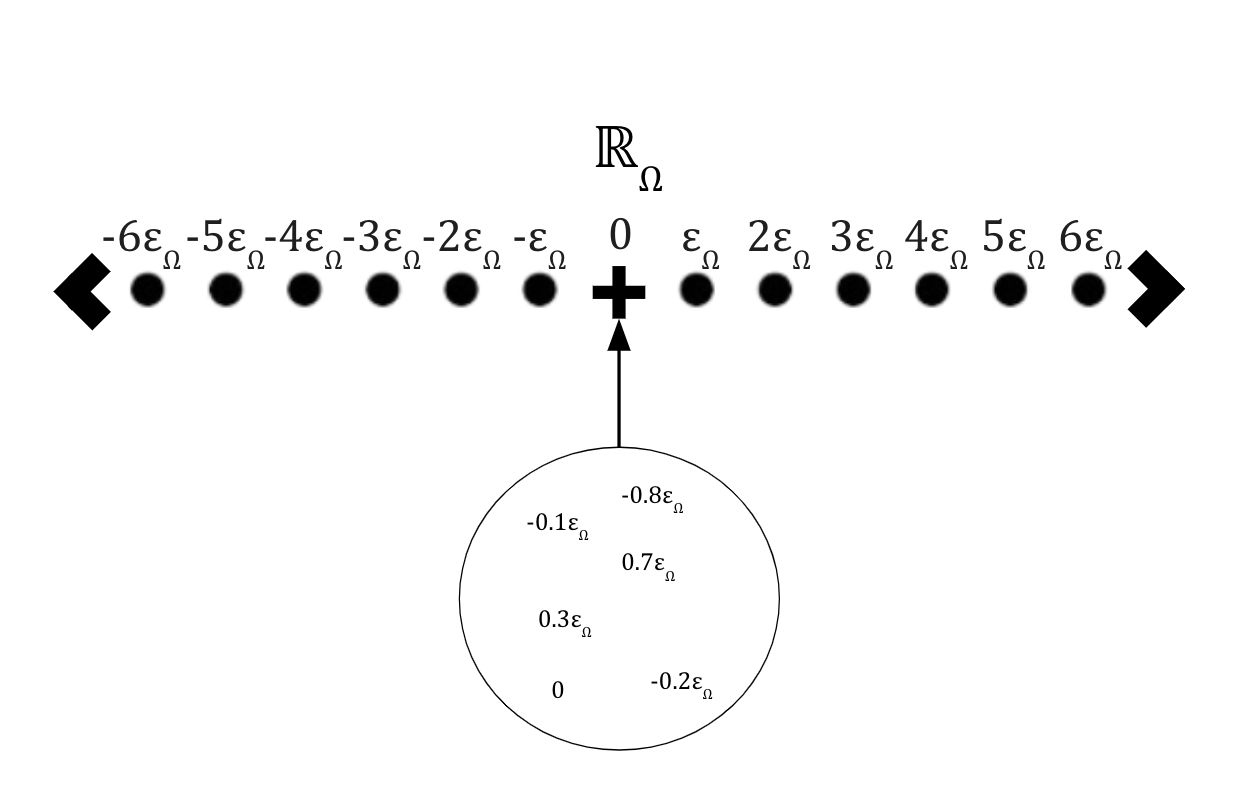
\includegraphics[width=1\linewidth]{Screenshot 2026-02-01 at 15.03.14.png}
                \caption{Different sub-infinitesimal data of zero}
    \label{fig:zero}
\end{figure} Note: 0 itself is included as a sub-infinitesimal data of 0, and this represents the traditional ``annihilator'' zero. This will be touched upon later.\\\\By consequence, the following diagram is \textbf{incorrect}, as it suggests $0.5\varepsilon_\Omega$ exists as a distinct point, even though $0.5\varepsilon_\Omega$ isn't a standalone element in $\mathbb{R}_\Omega$:
\begin{figure} [H]
    \centering
    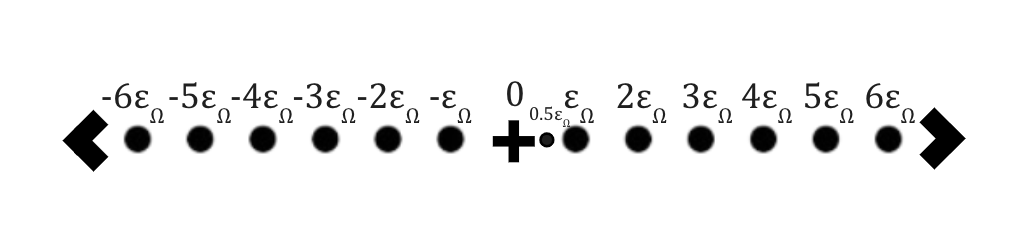
\includegraphics[width=1\linewidth]{Screenshot 2026-02-01 at 16.35.53.png}
    \caption{Wrong interpretation of the number line and of sub-infinitesimal data}
    \label{fig:placeholder}
\end{figure}
\\ 

A different example to understand this, is by considering the following expressions:
$$0.3\varepsilon_\Omega, \quad 0.8\varepsilon_\Omega, \quad \frac{7}{8}\varepsilon_\Omega, \quad 0.0001\varepsilon_\Omega, \quad -0.32\varepsilon_\Omega$$

They are all zero-equivalent expressions of 0, so they all have the same \textit{actual value}, but differ in \textit{data}:
\begin{align*}
0_{[0.3\varepsilon_\Omega]}\text{ }{}_a{=}_a \text{ }0_{[0.8\varepsilon_\Omega]}\text{ }{}_a{=}_a\text{ }0_{[\frac{7}{8}\varepsilon_\Omega]}\text{ } {}_a{=}_a\text{ } 0_{[0.0001\varepsilon_\Omega]}\text{ } {}_a{=}_a \text{ }0_{[-0.32\varepsilon_\Omega]}
\end{align*}
Because technically:
$$0 = 0 = 0 = 0 = 0$$This enforces the discrete nature of the absolute infinitesimal number line. Since values smaller than $\varepsilon_\Omega$ do not exist as actual magnitudes, there are no actual values between consecutive integer multiples of $\varepsilon_\Omega$. Instead, expressions like $0.5\varepsilon_\Omega$ exist as virtual sub-infinitesimal data of zero: they collapse to zero in actuality but are preserved as metadata.

\subsection{Sub-infinitesimal data properties}

Having established that sub-infinitesimal data is virtual information carried by zero when an absolute infinitesimal expression crosses the lower bound, we now examine how it actually \textit{behaves} in this framework. 

\subsubsection{Unsigned property}

Since all sub-infinitesimal data is equal to each other, and it is all zero-equivalent by nature, sub-infinitesimal data expressions, much like zero, are technically neutral: they are not actually negative nor positive. For example, the following two sub-infinitesimal data expressions of zero are equal by actuality, so by consequence, they are actually neutral, despite \textit{virtually} possessing signs.
$$0_{[0.3\varepsilon_\Omega]} \text{ }{}_a{=}_a \text{ } 0_{[-0.3\varepsilon_\Omega]} $$ This is because again, sub-infinitesimal data is like meta-data, it is not an actual value.

\subsubsection{Recovery of Magnitude}

The recovery of magnitude property is one of the most important properties of sub-infinitesimal data, as it represents the first step toward defining division by zero, as it fundamentally redefines zero's traditional role as a multiplicative annihilator, enabling \textbf{invertibility} - allowing absolute infinitesimal expressions which were collapsed to zero to recover their magnitude.
\\Traditionally, zero annihilates all magnitude: for any $n$,
$$0 \times n = 0$$ However, with sub-infinitesimal data, this immutable property becomes conditional, as sub-infinitesimal data allows zero to behave \textbf{like a non-zero number} in certain contexts, allowing for multiplication of zero to be able to yield non-zero results. This however, is purely conditional, and for zero to multiply out to a non-zero value, it has to carry sub-infinitesimal data. Consider what happens when an absolute infinitesimal is reduced by division:
$$\frac{\varepsilon_\Omega}{2} = 0$$In actual notation, this appears to equal zero. However, in virtual notation:
$$\frac{\varepsilon_\Omega}{2} =_v 0_{[0.5\varepsilon_\Omega]}$$ The resulting zero carries sub-infinitesimal data: it ``remembers'' having previously been $\varepsilon_\Omega$. When multiplied by 2, the vanished magnitude is then \textbf{recovered}:
$$0_{[0.5\varepsilon_\Omega]} \times 2\text{ } _v{=} \text{ }\varepsilon_\Omega$$ Why does this work? The data $[0.5\varepsilon_\Omega]$ encodes the relationship $0.5 \times 2 = 1$. When applied at the absolute infinitesimal scale, this yields $0.5\varepsilon_\Omega \times 2 = \varepsilon_\Omega$; the magnitude is recovered through virtuality.
In purely actual notation, this appears as:
$$0 \times 2 = \varepsilon_\Omega$$ This is counterintuitive, as it is paradoxical by traditional standards. One might object: ``But zero times anything \textit{must} be zero!'' This is true for the \textit{traditional} zero. However, $0_{[0.5\varepsilon_\Omega]}$ is not the traditional zero: it is a zero carrying virtual information that modifies its arithmetic behavior. In $\mathbb{R}_\Omega$, this is mathematically valid, provided the zero possesses the appropriate sub-infinitesimal data.

\subsubsection{The Initialization Requirement} For this recovery to occur, the zero must have been \textit{initialized}, created through the explicit previous reduction of an absolute infinitesimal. Zero does not arbitrarily acquire sub-infinitesimal data; it must inherit it from a prior operation, otherwise it functions traditionally. This property is context-specific: only zeros initialized with sub-infinitesimal data exhibit magnitude recovery. \\This is why declaration notation is essential for demonstration. For an expression like $0 \times 2 = \varepsilon_\Omega$ to hold, we must first establish:
$$0 \to_v 0_{[0.5\varepsilon_\Omega]}$$ This declares that the zero in question carries the specific sub-infinitesimal data $[0.5\varepsilon_\Omega]$, enabling magnitude recovery.
\subsubsection*{Example:}
To illustrate this property in action:
\begin{align*}
&\varepsilon_\Omega \div 3 =_v 0_{[\frac{\varepsilon_\Omega}{3}]} \text{ (initialization through division)}
\end{align*}
\begin{center}
$\updownarrow$
\end{center}
\begin{align*}
&0_{[\frac{\varepsilon_\Omega}{3}]} \times 3\text{ } _v{=} \varepsilon_\Omega \text{ (magnitude recovery)} 
\end{align*} The division creates sub-infinitesimal data; the multiplication recovers the original magnitude.
\\\\Crucially, what this also means is that sub-infinitesimal data cannot be artificially assigned. It is metadata inherent to a number's origins and must arise from an actual reduction operation. 
\\For example, the following is \textbf{invalid}:
\begin{align*}
&1 = 1 \\
&1 + 0 = 1 \quad \text{(adding arbitrary zero)} \\
&2\times(1 + 0_{[0.5\varepsilon_\Omega]}) \text{ } _v{=} \text{ }2 \times 1 \text{ (arbitrarily assigning this zero sub-infinitesimal data)} \\
&2 + \varepsilon_\Omega = 2 \text{ (distributing, and ``recovering'' the lost magnitude)}
\end{align*} One cannot claim the zero added in the second step carries sub-infinitesimal data, as this would recover magnitude that was never lost. For the left-hand side to contain sub-infinitesimal data, the original expression must have already possessed it. For instance, if the initial $1$ were initialized as $1 \to_v \frac{2\varepsilon_\Omega + 2}{2}$, then the expression would be valid. \\As a final note, if a zero has not been initialized, it is taken to be the ``default'' or ``traditional'' zero, with its ordinary properties of multiplicative annihilation. In virtual notation, an uninitialized (traditional) zero is written as $0_{[0]}$ or sometimes simply $0$. 

\subsection{The Distributivity Problem Revisited}

In Chapter 3, we observed that distributivity presents challenges in $\mathbb{R}_\Omega$. Expressions like $\varepsilon_\Omega \times (1 - 0.5)$ created ambiguity, whether evaluation of the interior first (obtaining $0.5\varepsilon_\Omega = 0$) or distribute first (obtaining $\varepsilon_\Omega - 0.5\varepsilon_\Omega=\varepsilon_\Omega$) was the correct choice. The answer wasn't evident, which was problematic, as this single problem threatened the notion of an absolute lower bound. The bound property resolved the first part of the issue, which was cementing that sub-infinitesimal expressions \textit{are} zero-equivalent (something the distributive property suggested otherwise), thereby establishing the fact that expressions below $\varepsilon_\Omega$ collapse to zero. However, the bound property alone did not fully solve distributivity, it only established \textit{that} magnitudes vanish, not \textit{how} distributivity functions at the boundary.
\\The resolution to this problem lies in understanding what sub-infinitesimal expressions actually represent.

\subsubsection{Sub-Infinitesimals Are Not Measures}

Consider a traditional real number like $0.9$. This number can be expressed in multiple equivalent ways:
$$0.9 = 1 - 0.1 = 2 - 1.1 = 0.5 + 0.4$$ These are all valid because 0.9 is a \textbf{measure}: a defined distance from zero on the number line. Changing the point of reference does not change what $0.9$ represents. Figure 6 illustrates this on the real number line:

\begin{figure} [H]
    \centering
    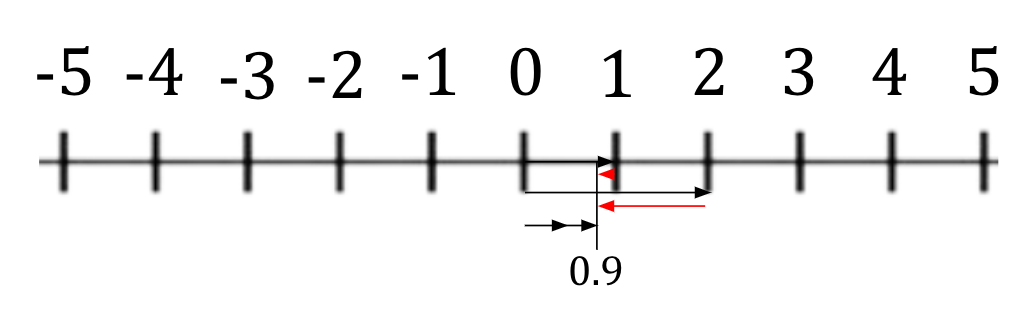
\includegraphics[width=1\linewidth]{Screenshot 2026-02-01 at 22.23.09.png}
    \caption{Multiple equivalent representations of 0.9 on the real number line.}
    \label{fig:placeholder}
\end{figure} In the first representation, we move forward 1 unit (black arrow) then back 0.1 units (red arrow). In the second, forward 2 units then back 1.1 units. In the third, forward 0.5 units then 0.4 units. All paths arrive at the same point: $0.9$.
\\The absolute infinitesimal number line however, is different, because it is discrete, with the only incrementing element being $\varepsilon_\Omega$:

\begin{figure} [H]
    \centering
    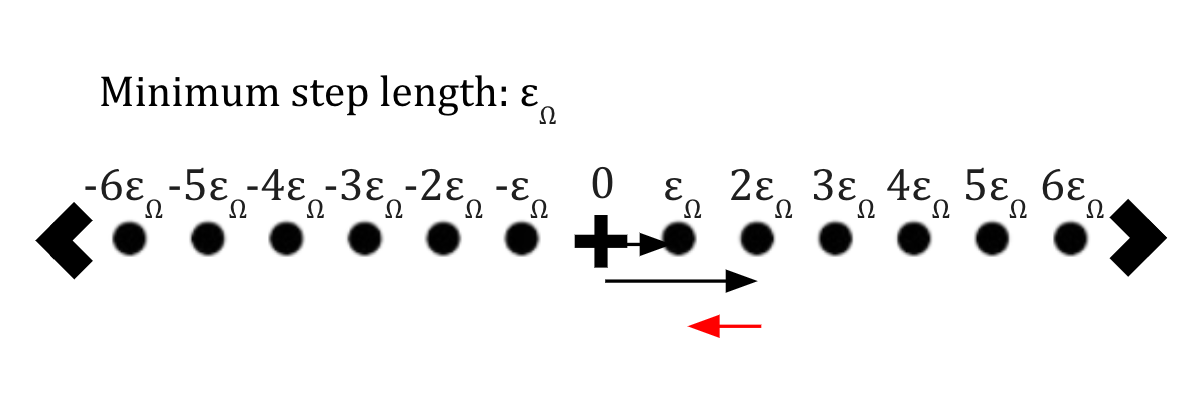
\includegraphics[width=1\linewidth]{Screenshot 2026-02-03 at 16.02.12.png}
    \caption{Attempting to reach a point that doesn't exist}
    \label{fig:placeholder}
\end{figure}

From Figure 7, re-consider the same arithmetic paths, now applied to the absolute 
infinitesimal number line where the minimum step length is $\varepsilon_\Omega$:

\begin{itemize}
    \item \textbf{Path 1:} $0 + \varepsilon_\Omega - 0.1\varepsilon_\Omega$ --- we move 
    forward one absolute infinitesimal unit, then attempt to step back $0.1\varepsilon_\Omega$. 
    But $0.1\varepsilon_\Omega < \varepsilon_\Omega$, so no backward movement occurs. 
    We land on $\varepsilon_\Omega$, not $0.9\varepsilon_\Omega$.
    
    \item \textbf{Path 2:} $0 + 2\varepsilon_\Omega - 1.1\varepsilon_\Omega$ --- we move 
    forward two units, then attempt to step back $1.1\varepsilon_\Omega$. The minimum 
    step is $\varepsilon_\Omega$, so we can only step back one unit. We land on 
    $\varepsilon_\Omega$, not $0.9\varepsilon_\Omega$.
    
    \item \textbf{Path 3:} $0 + 0.4\varepsilon_\Omega + 0.5\varepsilon_\Omega$ --- both 
    steps are below $\varepsilon_\Omega$, so neither movement occurs at all. We remain 
    at $0$. This path is not illustrated because no movement takes place.
\end{itemize}

None of these paths reach $0.9\varepsilon_\Omega$, and this is not a failure of 
arithmetic, but a structural fact: \textbf{$0.9\varepsilon_\Omega$ is not a point on 
this number line}. In the reals, $0.9$ is a destination that can be approached from 
any direction through infinitely many equivalent paths. In $\mathbb{R}_\Omega$, no such 
destination exists between $0$ and $\varepsilon_\Omega$. The arithmetic paths that 
would reach it in $\mathbb{R}$ simply snap to the nearest actual value which is 
either $0$ or $\varepsilon_\Omega$. This is precisely why sub-infinitesimal expressions 
cannot be redefined as compound arithmetic paths: there is no path to redefine, because 
there is no point to reach.
\\\\This demonstrates that:
$$0_{[0.9\varepsilon_\Omega]} \ {}_a{\neq}{}_a 
\ \varepsilon_\Omega - 0_{[-0.1\varepsilon_\Omega]}$$ Because $0.9\varepsilon_\Omega$ has no location as an actual value on the number line, it must be understood differently: not as a measure, but as \textbf{virtual data of zero}. \\\\Recall from figure 4 that sub-infinitesimal data does not occupy separate points on the number line, but rather exists as different ``flavors'' of zero within zero internally. Therefore, $0.9\varepsilon_\Omega$ should not be interpreted as ``nine-tenths of an absolute infinitesimal away from zero'', but rather as zero carrying metadata that behaves as if it \textit{\textbf{were}} nine-tenths of an absolute infinitesimal.
\\\\This distinction has consequences. While traditionally:
$$0.9 = 1 - 0.1$$In the context of sub-infinitesimal data:
$$0_{[0.9\varepsilon_\Omega]} \text{ }_a{\neq}{}_a \text{ }(1 - 0.1)\varepsilon_\Omega$$The left side, $0.9\varepsilon_\Omega$, is a sub-infinitesimal data expression: zero carrying specific metadata. The right side, $(1 - 0.1)\varepsilon_\Omega$, is an expression that \textit{evaluates to} $\varepsilon_\Omega$ actually, and $\varepsilon_\Omega-0_{[0.1\varepsilon_\Omega]}$ virtually.

\subsubsection{The Solution to Distributivity}

The resolution is now clear: \textbf{sub-infinitesimal expressions cannot be redefined as compound bracket expressions.}
\\\\While in the reals, $0.9 = 1 - 0.1$, in $\mathbb{R}_\Omega$:
$$0.9\varepsilon_\Omega \ {}_a{\neq}{}_a \ (1 - 0.1)\varepsilon_\Omega$$The transformation $n\varepsilon_\Omega \to (1-c)\varepsilon_\Omega$ is \textbf{invalid} because it attempts to rewrite virtual data as an arithmetic operation on actual values.\\Sub-infinitesimal data is not a measure that can be ``reached'' through different arithmetic paths. These two expressions have fundamentally different structures:
\begin{itemize}
\item $0.9\varepsilon_\Omega$ : Has actual value $0$ with sub-infinitesimal data: $0_{[0.9\varepsilon_\Omega]}$
\item $(1-0.1)\varepsilon_\Omega$ : Has actual value $\varepsilon_\Omega$ with sub-infinitesimal data: $\varepsilon_\Omega + 0_{[-0.1\varepsilon_\Omega]}$
\end{itemize}

This distinction resolves the distributivity paradox through three key points:
\begin{itemize}
\item \textbf{Different actual values}: $0.9\varepsilon_\Omega$ has actual value $0$, while $(1-0.1)\varepsilon_\Omega$ has actual value $\varepsilon_\Omega$. Since their actualities differ, they cannot be equal.
\item \textbf{Virtual data is not arithmetic}: Sub-infinitesimal data arises when arithmetic operations cause a value to cross the lower bound of actuality in $\mathbb{R}_\Omega$. Once generated through boundary crossing, this data cannot be algebraically reconstructed: you cannot ``build'' $0.9\varepsilon_\Omega$ by performing $1 - 0.1$ on $\varepsilon_\Omega$ because the data already exists from a prior boundary event, not from this specific calculation.
\item \textbf{Redefinition is invalid}: The transformation $n\varepsilon_\Omega \to (1-c)\varepsilon_\Omega$ attempts to rewrite virtual data as an arithmetic expression, which violates the fundamental nature of sub-infinitesimal data.
\end{itemize}

Therefore, you cannot distribute over sub-infinitesimal data because it is not composed of arithmetic operations: it is virtual data, not actual value.

\subsubsection*{Exception: Square Bracket Notation}

However, there exists one important exception where bracket notation becomes essential.
\\In $\mathbb{R}_\Omega$, numbers like $1 - \varepsilon_\Omega$ exist as actual values 
on the number line, but cannot be expressed cleanly in decimal form --- doing so would 
require an absolute hyperfinite string of 9's whose final digit(s) are unknowable, 
since there is no way to prove that $\varepsilon_\Omega$ is a power of 10.\footnote{If 
$\varepsilon_\Omega$ were hypothetically some multiple of a large prime, the decimal 
expansion would have an entirely non-trivial tail structure, making the last digit(s) 
provably undeterminable.}
\\For sub-infinitesimal expressions involving $1 - z\varepsilon_\Omega$ where $z$ is a positive integer, we use \textbf{square bracket notation}:
$$[1 - \varepsilon_\Omega]\varepsilon_\Omega$$

This is a sub-infinitesimal expression with actual value zero:
$$0_{[1 - \varepsilon_\Omega]\varepsilon_\Omega}$$
\\Square brackets indicate: ``evaluate the interior as written; do not expand or distribute.'' This preserves the mathematical properties without requiring impossible decimal representation.
\\Crucially, $[1 - \varepsilon_\Omega]\varepsilon_\Omega$ has actual value $0$, while $(1 - \varepsilon_\Omega)\varepsilon_\Omega$ has actual value $\varepsilon_\Omega$.

\subsubsection{Same Data, Different Actual Values}

But \textit{what exactly do} we mean when we claim that $0.9\varepsilon_\Omega$ and $(1-0.1)\varepsilon_\Omega$ are different? That one represents sub-infinitesimal data of zero, while the other is an actual value combined with a zero carrying sub-infinitesimal data?
\\The distinction lies in their actual values: $0.9\varepsilon_\Omega$ has actual value 0, whereas $(1-0.1)\varepsilon_\Omega$ has actual value $\varepsilon_\Omega$. Since $0\neq\varepsilon_\Omega$, these expressions are not actually equal.
\\\textit{However}, despite possessing different magnitudes, these two numbers share the same \textbf{data}, and consequently exhibit the same \textbf{mathematical properties}.
\\Consider the two expressions again. In actual notation:
$$0\neq\varepsilon_\Omega$$
$$\updownarrow$$
$$\varepsilon_\Omega - 0_{[0.1\varepsilon_\Omega]} \ {}_a{\neq}{}_a \ 0_{[0.9\varepsilon_\Omega]}$$

Despite being distinct actual values, they possess the \textbf{same arithmetical properties}. This means they demonstrate identical arithmetic behavior while maintaining different magnitudes:
$$\varepsilon_\Omega\to_v \varepsilon_\Omega+0_{[-0.1\varepsilon_\Omega]}$$
$$\varepsilon_\Omega \times 10=9\varepsilon_\Omega$$
$$0\to_v0_{[0.9\varepsilon_\Omega]}$$
$$0\times 10=9\varepsilon_\Omega$$

Although $\varepsilon_\Omega+0_{[-0.1\varepsilon_\Omega]} \ {}_a{\neq}{}_a \ 0_{[0.9\varepsilon_\Omega]}$, their shared property of multiplication by ten resulting in the same actual value make it so we write a \textit{virtual} equality, $\varepsilon_\Omega+0_{[-0.1\varepsilon_\Omega]} \ {}_v{=}{}_v \ 0_{[0.9\varepsilon_\Omega]}$. This precisely means that $\varepsilon_\Omega+0_{[-0.1\varepsilon_\Omega]}$ is a sub-infinitesimal data expression of $\varepsilon_\Omega$, while $0.9\varepsilon_\Omega$ is a sub-infinitesimal data expression of 0. They are different actual values that share the \textbf{same arithmetical properties}. Figure 8 illustrates this phenomenon by showing the sub-infinitesimal data of both zero and $\varepsilon_\Omega$ on the number line.

\begin{figure}[H]
    \centering
    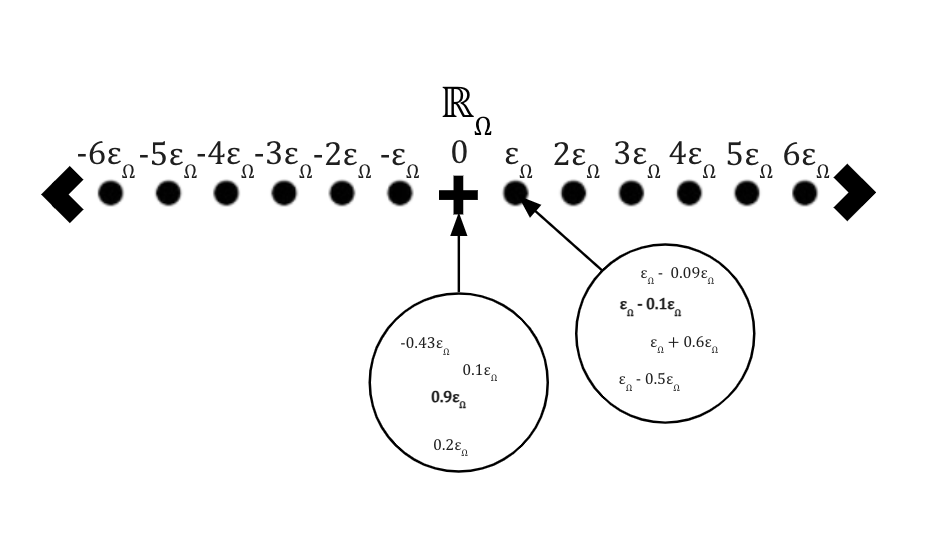
\includegraphics[width=1\linewidth]{Screenshot 2026-02-03 at 17.39.39.png}
    \caption{Sub-Infinitesimal Data of Different Actual Values}
    \label{fig:placeholder}
\end{figure}

The expressions in bold share the same data. This leads to two fundamental principles in $\mathbb{R}_\Omega$:
\begin{itemize}
\item Numbers with different actual values can have the same data
\item Numbers with the same actual value can have different data 
\end{itemize}Essentially, sub-infinitesimal data is not exclusive to zero. Any number $r$ can carry it through the form $r+0_{[d]}$, where adding zero preserves the actual value but introduces virtual data (only if this number was \textbf{initialized}  with sub-infinitesimal data first). For instance, $\frac{1+\varepsilon_\Omega}{2}$ yields actual value $0.5$ but virtual data $0.5+0_{[0.5\varepsilon_\Omega]}$.\footnote{An analogy of $0.9\varepsilon_\Omega$ and $\varepsilon_\Omega - 0.1\varepsilon_\Omega$ is that they are like two different foods that taste identical - they are distinct objects with equivalent properties.}

\subsubsection*{Additive Identity Preserved}

It is worth noting that sub-infinitesimal data does not affect zero's role as an 
additive identity. For any $a$:
$$a + 0_{[n\varepsilon_\Omega]} = a$$
This is because sub-infinitesimal data does not constitute actual magnitude: it 
only modifies arithmetic behavior under specific operations. Adding a zero, even one 
carrying sub-infinitesimal data, contributes nothing to actual value.
\newpage

\section{Chapter 6 - Infinity and Specific Infinite Data}

Of all the concepts reinterpreted in this theory, infinity undergoes the most 
radical transformation. Infinity in this framework is conceptually described as being less of a simple refinement of its traditional definition and is more of
a complete re-conceptualization from the ground up. This complete re-conceptualization arises because 
unlike sub-infinitesimal data, which extends zero, which is a well-understood number,  
specific infinite data extends \textbf{infinity}, which is traditionally not 
considered a number at all.

\subsection{Traditional Infinity}

In the reals, infinity is better understood as a \textit{direction} rather than a 
\textit{destination}; ``endlessly to the right'' or ``endlessly to the left'' 
rather than an actual value one can arrive at. This directional nature has a direct 
consequence: if a quantity is already endless, no finite operation can meaningfully 
alter it. Adding or subtracting a finite amount from something unbounded leaves it 
unbounded; multiplying it by a positive finite value leaves it endless in the same 
direction, and by a negative value reverses that direction:
\begin{align*}
\infty + x &= \infty \\
\infty - x &= \infty \\
\infty \cdot x &= \infty \quad (x > 0)\\
\infty \cdot x &= -\infty \quad (x < 0)\\
\infty - \infty &= \text{undef}\\
\frac{\infty}{\infty} &=\text{undef}
\end{align*}
Yet this places infinity in a peculiar position; fundamental to mathematical reasoning, yet somehow above the rules that govern ordinary numbers.

\subsection{Infinity in This Theory}

In this theory, infinity is fundamentally reimagined: it is reached when crossing the upper bound, because \textbf{actuality collapses beyond the upper bound}. For this, infinity is no longer imagined as a point or direction on the number line, but rather as a \textit{space} surrounding it conceptually analogous to how outer space surrounds a planet.

\begin{figure}[H]
    \centering
    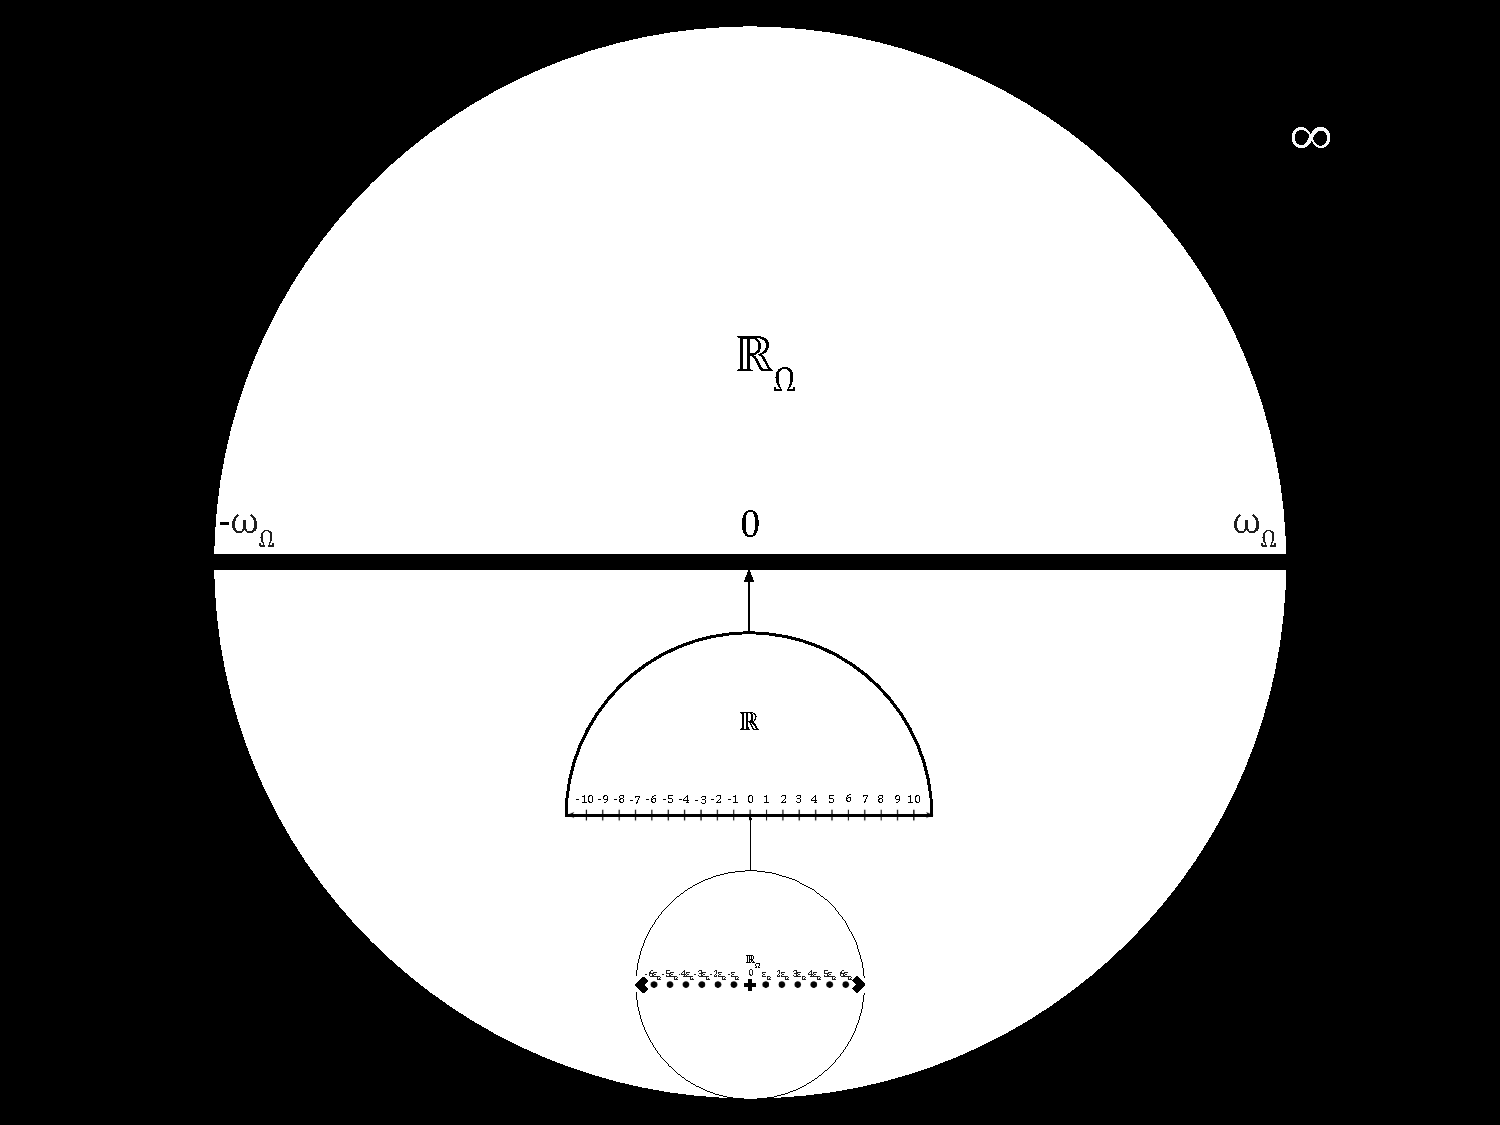
\includegraphics[width=1\linewidth]{Untitled drawing.pdf}
    \caption{The absolute hyper-reals at the absolute hyperfinite scale}
    \label{fig:placeholder}
\end{figure}

This spatial interpretation indicates that infinity is not an element of the absolute hyper-reals, which is why $\mathbb{R}_\Omega$ is not a field.
\begin{center}
$\infty \notin \mathbb{R}_\Omega$
\end{center}

Rather than extending the line to reach infinity, we declare it to be a fundamentally 
separate mathematical construct, in which it is defined as being a space surrounding the absolute hyper-reals rather 
than a point beyond them.
\\Yet infinity in this framework is also treated as \textbf{an actual value}: the value 
obtained when one exceeds $\omega_\Omega$, much like how certain programming languages 
return ``infinity'' upon overflow. It is not an element of $\mathbb{R}_\Omega$, but it 
is a definite result. Infinity is not some undefined value, as it is defined as having an actuality of ``infinity'' - \textit{beyond} the continuum.
\\When considering an ``uninitialized'' infinity in this framework (meaning \textbf{just} the actuality \textit{without} any prior specific infinite data initialization), infinity is described as retaining its traditional algebraic properties from the extended reals:
\begin{align*}
\infty + x &= \infty \\
\infty - x &= \infty \\
\infty \times x &= \infty \quad (x > 0)\\
\infty \times x &= -\infty \quad (x < 0)
\end{align*}

This dual conception of defining infinity as both a spatial boundary and an actual value, provides several conveniences absent from traditional definitions. 

\subsubsection{Unsigned Infinity}

In the extended reals, infinity is signed: $+\infty$ lies to the right, $-\infty$ to the left. This makes sense when infinity is conceived as a destination reached by traveling along the line.
\\But if infinity is a space \textit{enveloping} the number line rather than a point \textit{on} it, the notion of sign loses coherence. One cannot meaningfully describe infinity as a positive or negative distance from zero when it surrounds the line from all directions. Infinity in this theory is therefore unsigned - describable only as an absolute distance, not a signed one.
\\\\The absolute hyperfinite $\omega_\Omega$ therefore functions as the limit of length for a single dimension in any direction: beyond this bound, actuality breaks down, and the number line is conceptually described as ``not being able to extend further''. At infinity, traditional notions of geometry, direction and distance lose meaning, reinforcing the interpretation of infinity as a space - as no matter how you exit the number line (left, right, up, down, inwards or outwards), the moment your absolute distance breaches $\omega_\Omega$, you've reached infinity, where the traditional rules established in $\mathbb{R}_\Omega$ break down.

\subsubsection{Infinity as Boundary Value}

Traditionally, infinity is unbounded, as it is unaffected by ordinary operations. This theory retains that property: infinity remains conceptually boundless and neverending.
\\Yet infinity is \textit{also} defined as the value achieved when the upper bound $\omega_\Omega$ is crossed. $$k > |1| \implies k \times \omega_\Omega = \infty$$This creates an apparent contradiction: how can something be truly infinite if reaching it requires only breaching a finite value by a finite amount?
\\This is precisely where specific infinite data becomes essential, as it mediates 
between infinity as a boundless concept and infinity as a boundary crossing, allowing 
both interpretations to coexist inside one entity. This refinement enables algebraic manipulations of 
infinity that traditional definitions would never permit.

\subsubsection{Closure of the Algebraic Structure}

The absolute reals $\mathbb{R}_\Omega$ form an open algebraic structure: breaching the upper bound takes you outside the system. But the union with this spatial infinity closes that openness.
\\The resulting structure $\mathbb{R}_\Omega \cup \{\infty\}$ resembles a field more closely: though calling it a field would be inaccurate, since division by zero is defined (and traditional fields explicitly leave $\frac{a}{0}$ undefined).
\\This closure was described as being the first step toward defining division by zero, as it establishes the identity of infinity and zero being reciprocal identities of each other \textbf{by actuality}. However, to fully understand this relationship requires the development of specific infinite data.

\subsection{Specific Infinite Data}

Having re-established the conceptual origins of infinity in this number system, we now examine how infinity operates through \textbf{specific infinite data}, which is the infinite analog of sub-infinitesimal data.

\subsubsection{Definition and Duality}

Just as zero can carry sub-infinitesimal data, infinity can carry \textbf{specific infinite data}. This duality mirrors the structure we established for zero:

\begin{itemize}
\item \textbf{Actuality}: Infinity has actual value $\infty$, with traditional properties: it is boundless and neverending.
\item \textbf{Virtuality}: When the upper bound $\omega_\Omega$ is crossed, the resulting number has actuality $\infty$ but carries virtual data corresponding to what the value ``would have been''.
\end{itemize}

In virtual notation, specific infinite data is written as:
$$\infty_{[k\omega_\Omega]}$$In which $k>|1|$. This infinity has actual value $\infty$ but possesses the arithmetic properties of $k\omega_\Omega$. In actual notation (using standard equality $=$), virtuality is hidden and the expression is simply $\infty$.

As an example:

$$\omega_\Omega\times5=\infty$$$$\updownarrow$$
$$\omega_\Omega\times5=_v\infty_{[5\omega_\Omega]}$$

Traditional infinity without specific data is denoted $\infty_{[\infty]}$ in virtual notation, analogous to $0_{[0]}$ for traditional zero.

\subsubsection{No Independent Values Above $\omega_\Omega$}

A crucial principle mirrors that of sub-infinitesimal data: just as sub-infinitesimal 
expressions are not standalone elements of $\mathbb{R}_\Omega$, specific infinite data 
expressions are \textit{also} not standalone elements of $\infty$, as \textbf{there is only one actual value above the absolute hyperfinite, and that is $\infty$}. This means that any expression whose magnitude exceeds $\omega_\Omega$ does not exist as an independent actual value (or point on a line) they only exist as a \textbf{virtual specific infinite data} that infinity carries depending on context. Values above $\omega_\Omega$ are not points on a number line; they are different ``flavors'' of infinity. 
\\One interpretation is to envision specific infinite data expressions as 
\textit{labels} for the same undifferentiated space, much like how multiple 
names for the same place do not create multiple places. $5\omega_\Omega$, 
$-234\omega_\Omega$, and $999\omega_\Omega$ are not different locations within 
infinity; they are different ways of arriving at the same destination. The black 
space in Figure 10 is not populated by these expressions, it simply \textbf{is} 
infinity, and these expressions are descriptions of it, not constituents of it. Infinity is best understood as a unified space that carries all of these labels 
simultaneously: not a collection of distinct points, but a single undifferentiated 
expanse that every specific infinite expression refers to at once.

\begin{figure} [H]
    \centering
    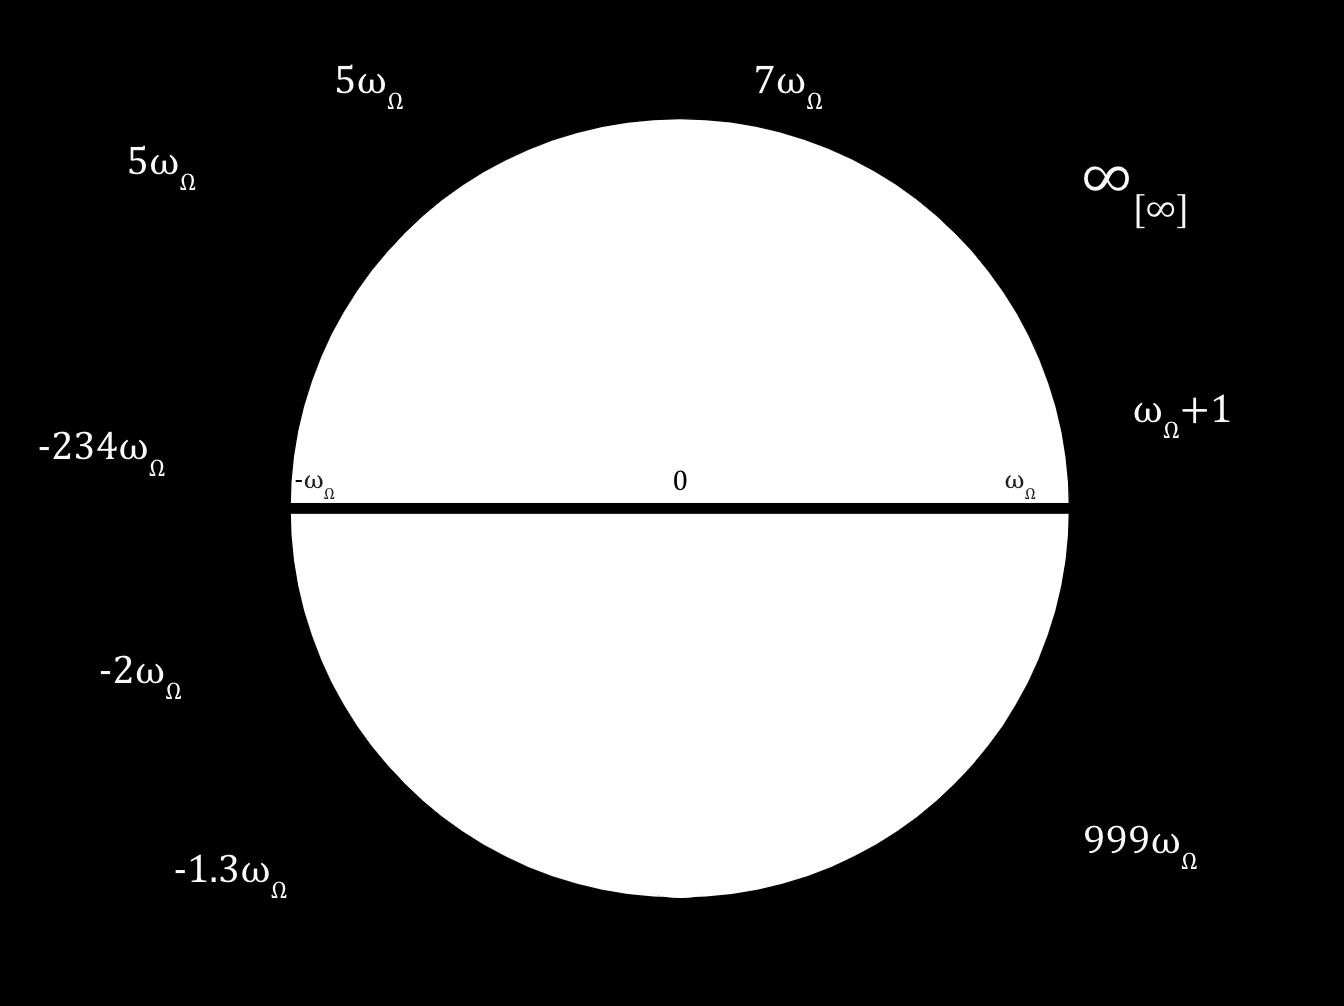
\includegraphics[width=1\linewidth]{Screenshot 2026-02-03 at 22.13.55.png}
    \caption{Virtual Infinite Space}
    \label{fig:placeholder}
\end{figure}

Just as sub-infinitesimal data represents different flavors of zero, specific infinite data represents different flavors of infinity. All such expressions are just different ``metadata'' to the same actual value of $\infty$.
\\This reinforces the spatial interpretation of infinity: these data expressions do 
not exist as independent points on a line, nor do they combine to form infinity. 
Rather, infinity is the space itself, singular and undifferentiated, and 
specific infinite data expressions are simply different labels for the same whole.

\subsubsection{Actual Equality and Virtual Inequality}

All specific infinite data are equal in \textbf{actuality} to each other but differ in \textbf{virtuality}.
For example:
$$\infty_{[\omega_\Omega+4]} \ {}_a{=}_a \ \infty_{[-\omega_\Omega-8]} \ {}_a{=}_a \ \infty_{[2\omega_\Omega]} \ {}_a{=}_a \ \infty_{[9\times10^{1000}\omega_\Omega]}$$ Because,
$$\infty=\infty=\infty=\infty$$ However, these different specific infinite data expressions are \textit{different in virtuality}:
$$\infty_{[\omega_\Omega+4]} \ {}_v{\neq}{}_v \ \infty_{[-\omega_\Omega-8]} \ {}_v{\neq}{}_v \ \infty_{[2\omega_\Omega]} \ {}_v{\neq}{}_v \ \infty_{[9\times10^{1000}\omega_\Omega]}$$

\subsubsection{Context-Specificity and Initialization}

Like sub-infinitesimal data, specific infinite data does not exist independently: 
it arises only from \textbf{crossing the upper bound of the absolute hyper-reals}. 
When an operation causes a value to exceed $\omega_\Omega$, the result has actual 
value $\infty$ but carries virtual data corresponding to what the value ``would 
have been.'' Specific infinite data is context-specific: it is not a free-floating 
independent value that exists prior to any operation, but always the result of a 
particular boundary-crossing event.

\subsubsection{Reciprocal Relationship with Sub-Infinitesimal Data}

Specific infinite data expressions act as direct reciprocals to sub-infinitesimal data expressions. This reciprocal relationship is foundational to how the bound property functions: every zero-equivalent sub-infinitesimal expression has a matching infinite-equivalent specific infinite expression.
\\ 
For example:
\begin{align*}
&\frac{1}{0_{[0.5\varepsilon_\Omega]}} \ {}_v{=}{}_v \ \infty_{[2\omega_\Omega]} \\
&\frac{1}{0_{[0.01\overline{38}\varepsilon_\Omega]}} \ {}_v{=}{}_v \ \infty_{[72\omega_\Omega]}
\end{align*}

This relationship holds as an identity by actuality, so for any sub-infinitesimal and specific infinite data:
$$\frac{1}{\infty} = 0 \quad\text{and} \quad \frac{1}{0}=\infty$$No matter what the specific data of infinity is, dividing 1 by it always yields a zero-equivalent sub-infinitesimal expression. This is true whether the data represents expressions ``close'' to the continuum ($\infty_{[\omega_\Omega + 1]}$) or ``far'' from it ($\infty_{[52!\omega_\Omega]}$), although we must remember that distance and proximity are meaningless in the spatial interpretation of infinity.

\subsubsection{Limit Replacement}

This reciprocal relationship enables the idea of replacing the concept of a \textit{limit}: instead of describing functions approaching infinity or zero, we can directly evaluate functions at zero-equivalent sub-infinitesimal expressions or infinite-equivalent specific infinite expressions\footnote{Although we introduce the concept here, calculus in $\mathbb{R}_\Omega$ will be discussed in further detail in chapter 11.}.
\\\\Consider the function:
$$f(x) = \frac{1}{x}$$

Traditionally, $f(x)$ is undefined at 0 and approaches 0 as $x \to \infty$:
$$\lim_{x \to \infty} f(x) = 0 \qquad \lim_{x \to 0^+} f(x) = \infty$$

In this theory, limits are reinterpreted through boundary crossings:
\begin{itemize}
\item Crossing the lower bound (magnitude below $\varepsilon_\Omega$) yields sub-infinitesimal data
\item Crossing the upper bound (magnitude above $\omega_\Omega$) yields specific infinite data
\end{itemize}

This allows us to directly evaluate the functions at those points \textit{virtually}:
$$f(\infty) = 0 \qquad f(0) = \infty$$
$$\updownarrow$$
$$f(\infty_{[k\omega_\Omega]}) \ _a{=}{}_a \ 0_{[n\varepsilon_\Omega]} \qquad f(0_{[n\varepsilon_\Omega]}) \ _a{=}{}_a \ \infty_{[k\omega_\Omega]}$$
In which $k>|1|$ and $n=\frac{1}{k}$, because for any \textit{specific infinite data} expression, there exists a corresponding \textit{sub-infinitesimal data} expression.
For example, choosing one sub-infinitesimal expression, we get:
\begin{align*}
f(\infty_{[2\omega_\Omega]}) &\ {}_a{=}_a \ 0_{[0.5\varepsilon_\Omega]} \\
f(\infty_{[-2\omega_\Omega]}) &\ {}_a{=}_a \ 0_{[-0.5\varepsilon_\Omega]}
\end{align*}

By actual value: $f(\infty) = 0$.

Similarly, at the sub-infinitesimal level:
\begin{align*}
f(0_{[0.5\varepsilon_\Omega]}) &\ {}_a{=}_a \ \infty_{[2\omega_\Omega]} \\
f(0_{[-0.5\varepsilon_\Omega]}) &\ {}_a{=}_a \ \infty_{[-2\omega_\Omega]}
\end{align*}

\begin{figure} [H]
    \centering
    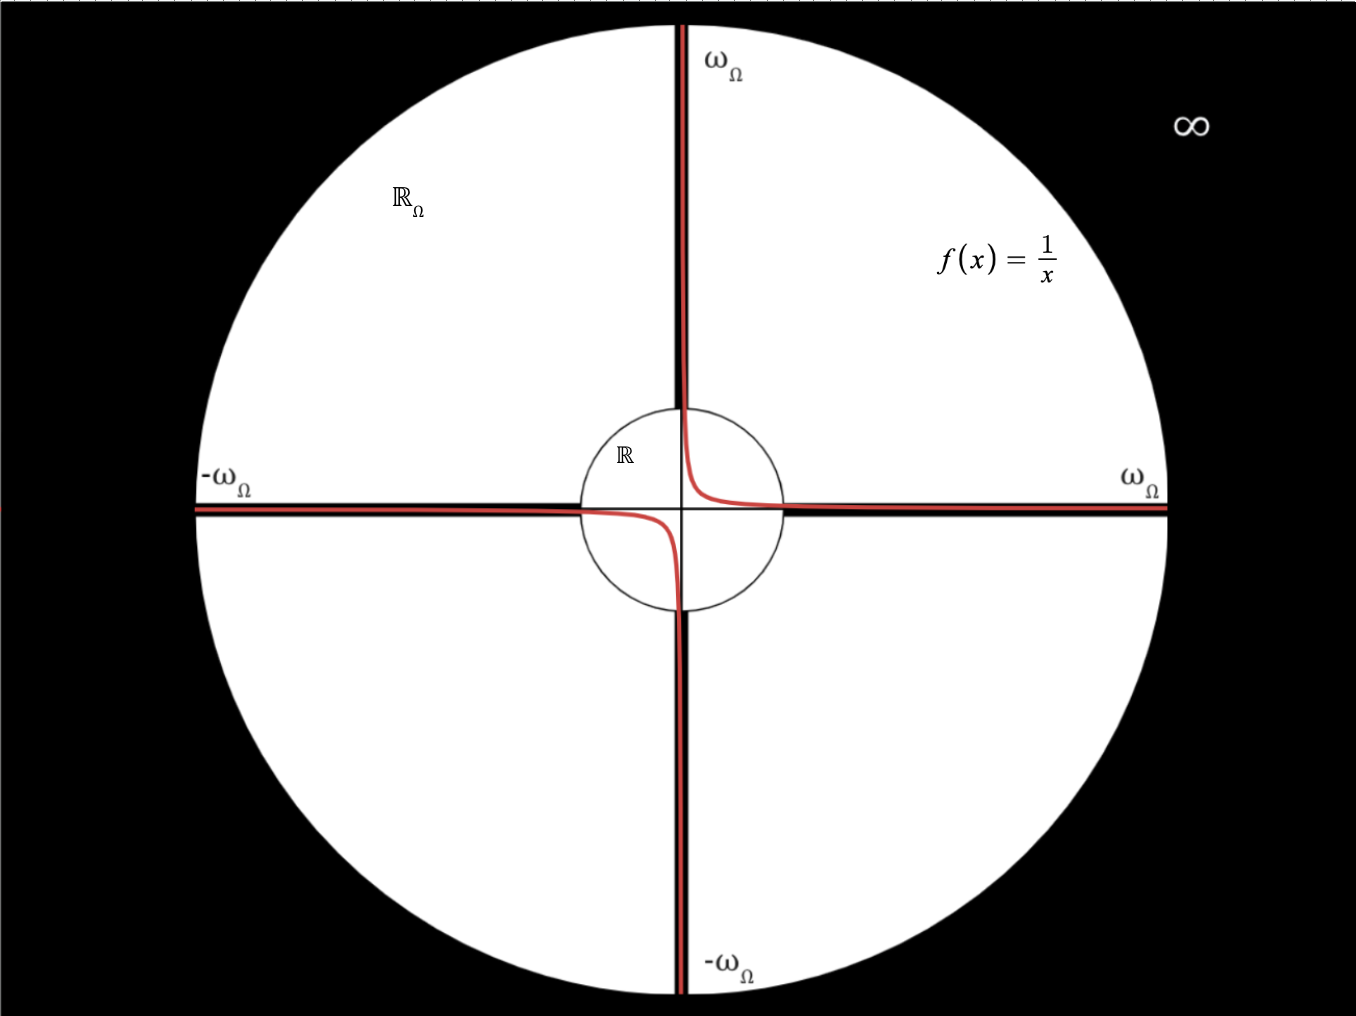
\includegraphics[width=1\linewidth]{Screenshot 2026-02-03 at 23.25.05.png}
    \caption{The reciprocal function within the absolute hyper-reals.}
    \label{fig:placeholder}
\end{figure}

Interestingly, just as in traditional limits, the function never technically crosses the $x$ and $y$ axes, because the axes themselves do not extend past $\omega_\Omega$. The function approaches but never reaches the axes within the visible continuum.

\subsubsection*{Note on directionality} In traditional analysis, $\lim_{x \to 0^+} \frac{1}{x} = +\infty$ while $\lim_{x \to 0^-} \frac{1}{x} = -\infty$, requiring separate treatment of left and right limits, making the function \textit{undefined at zero}. In this theory, due to the fact that infinity is unsigned and exists as a space surrounding the continuum rather than as directional points, both functions, despite going different directions, both \textbf{reach the same infinite space}. Rather than remaining undefined at zero, the function is now defined as infinity, with its behavior specified through specific infinite data. The traditional distinction between ``positive infinity'' and ``negative infinity'' collapses: there exists only $\infty$, distinguished by different virtuality. Thus $f(0_{[0.5\varepsilon_\Omega]}) = \infty_{[2\omega_\Omega]}$ and $f(0_{[-0.5\varepsilon_\Omega]}) = \infty_{[-2\omega_\Omega]}$ are both simply $\infty$ in actual value, differing only in their virtual data.

\subsubsection{Return to Finiteness Property}

One of the most important properties of specific infinite data, much like sub-infinitesimal data, is that it allows for infinity with specific data to be arithmetically manipulated to \textbf{produce finite values}.
\\This is analogous to how zero with sub-infinitesimal data can deviate from zero-like behavior. For example, if we had an infinity which was initialized to be:
$$\infty\to_v \infty_{[72\omega_\Omega]}$$ It would have the arithmetic property of:
$$\frac{\infty}{72} =\omega_\Omega$$
In this very specific context, having infinity returning a finite value is acceptable in this theory, because this infinity is the result of a crossing of the upper bound of actuality in this number system. This corresponding actual infinity will possess the virtuality of being $72\omega_\Omega$, which when divided by 72 returns the expression to finiteness $\omega_\Omega$.

\newpage
\section{Chapter 7 - Introduction to Absolute Infinitesimal Geometry}

The preceding chapters established the algebraic and data-theoretic foundations 
of $\mathbb{R}_\Omega \ \cup \ \infty$: the bound property, sub-infinitesimal data, specific 
infinite data, and the reciprocal relationship between them:
\begin{align*}
\frac{1}{0_{[n\varepsilon_\Omega]}} &= \infty_{[k\omega_\Omega]} \\
\frac{1}{\infty_{[k\omega_\Omega]}} &= 0_{[n\varepsilon_\Omega]}
\end{align*}
which in actual notation translates to:
\begin{align*}
\frac{1}{0} &= \infty \\
\frac{1}{\infty} &= 0
\end{align*}
These foundations are essential, however, they alone do not address division by zero fully. They address only \textbf{conditional} division by zero, which are division of 1 by zeroes carrying sub-infinitesimal data. The traditional zero $0_{[0]}$, possessing its original multiplicative annihilator property, remains undefined as a divisor. Which raises the question: can division by the \textit{traditional} zero, the one which has been come to be understood as undefinable, truly be defined? Can we give meaning to $\frac{1}{0_{[0]}}$, not merely to $\frac{1}{0_{[n\varepsilon_\Omega]}}$?
\\\\Within this framework, the answer is yes, but the path to this definition requires geometry, not arithmetic alone. The method presented in the following three chapters defines division by traditional zero through a synthesis of absolute infinitesimals, sub-infinitesimal data, infinity, specific infinite data, and a new form of mathematical metadata: \textbf{geometric data}. 

\subsection{Algebraic vs. Geometric $\mathbb{R}_\Omega$}

Throughout this theory, $\mathbb{R}_\Omega$ has been treated as an algebraic 
object: a number system with a lower bound $\varepsilon_\Omega$, an upper bound 
$\omega_\Omega$, and elements ranging from $-\omega_\Omega$ to $+\omega_\Omega$. 
This algebraic $\mathbb{R}_\Omega$ is what underlies the bound property, 
sub-infinitesimal data and specific infinite data. However, when we extend $\mathbb{R}_\Omega$ to geometric space, 
something important changes.
\\\\The algebraic $\mathbb{R}_\Omega$ spans from $-\omega_\Omega$ to 
$+\omega_\Omega$, giving it a total signed extent of $2\omega_\Omega$. 
This causes no algebraic contradiction, because the upper bound 
$\omega_\Omega$ was always defined as a bound on \textit{magnitude} 
$|x|$, not on signed value, and $2\omega_\Omega$ is a geometric measurement, not an algebraic one. Every element of $\mathbb{R}_\Omega$ 
satisfies $|x| \leq \omega_\Omega$ by definition. In geometry, however, 
length is inherently unsigned, which is where the distinction 
between \textit{algebraic} and \textit{geometric} $\mathbb{R}_\Omega$ becomes meaningful.

\begin{figure} [H]
    \centering
    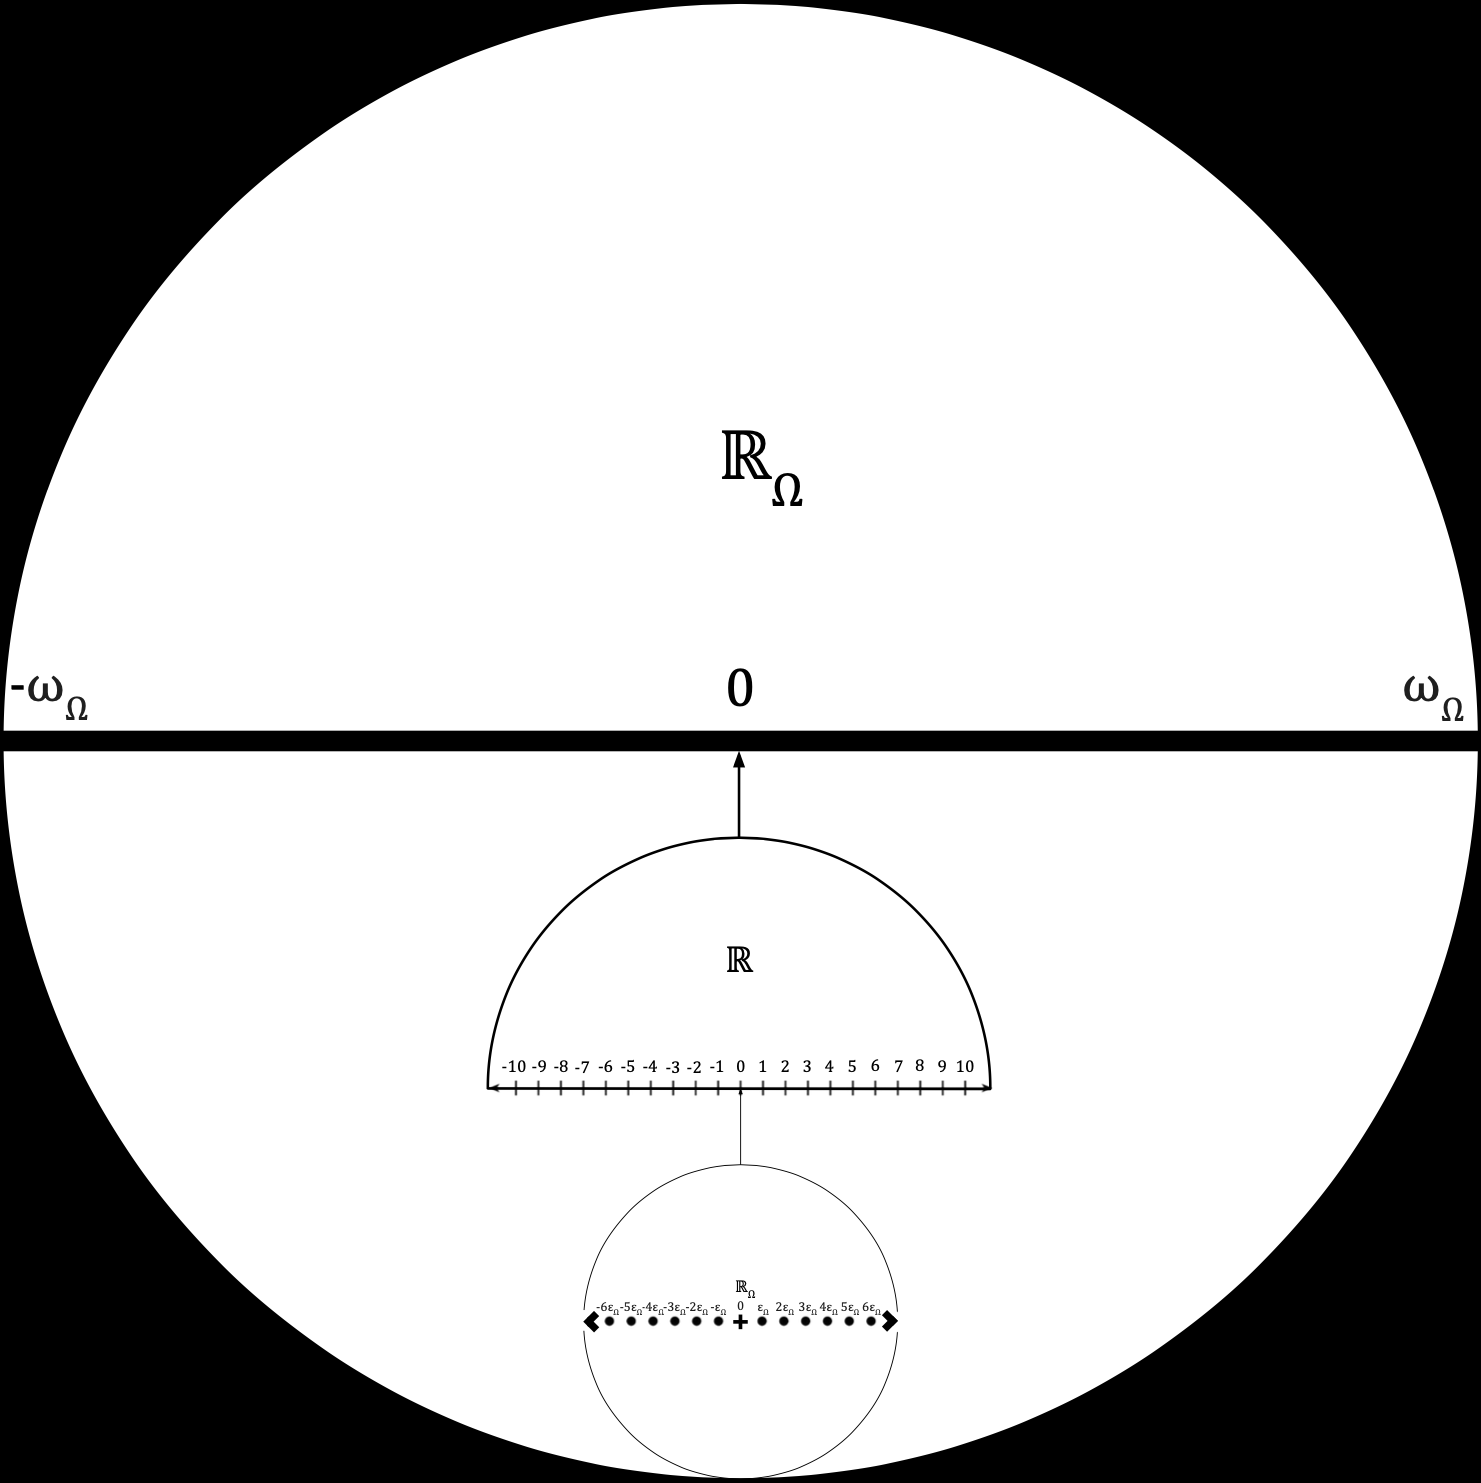
\includegraphics[width=1\linewidth]{Screenshot 2026-03-18 at 02.03.02.png}
    \caption{The algebraic $\mathbb{R}_\Omega$, spanning $-\omega_\Omega$ 
    to $+\omega_\Omega$ with total length $2\omega_\Omega$.}
    \label{fig:placeholder}
\end{figure}


In geometry, ``negative'' loses its meaning entirely. There is no 
such thing as a negative distance : only a distance in a particular direction. 
Every geometric measurement is an absolute distance from some reference point. 
This means that the geometric realisation of $\mathbb{R}_\Omega$ is not a 
signed line spanning $2\omega_\Omega$, but an unsigned continuum of absolute 
length $|\omega_\Omega|$. In geometric space, the concept of ``negative'' ceases to exist 
entirely. There is no negative half of the geometric continuum:  
only positions at varying absolute distances from a chosen origin. 
What algebra labels as ``$-3$'' is, geometrically, simply a point 
at distance 3 from the origin in one direction; the sign is a 
notational convention, not a geometric property. The geometric 
$\mathbb{R}_\Omega$ - which shall be labelled as $\mathbb{R}_\Omega^1$ moving forward to denote it's dimensionality, is therefore an unsigned continuum of absolute 
length $|\omega_\Omega|$, with the $+$ and $-$ labels in Figure 12 
serving only to indicate position relative to the origin (which was arbitrarily moved to the ``center'' of this continuum) - not 
to assert that negative magnitude exists.

\begin{figure} [H]
    \centering
    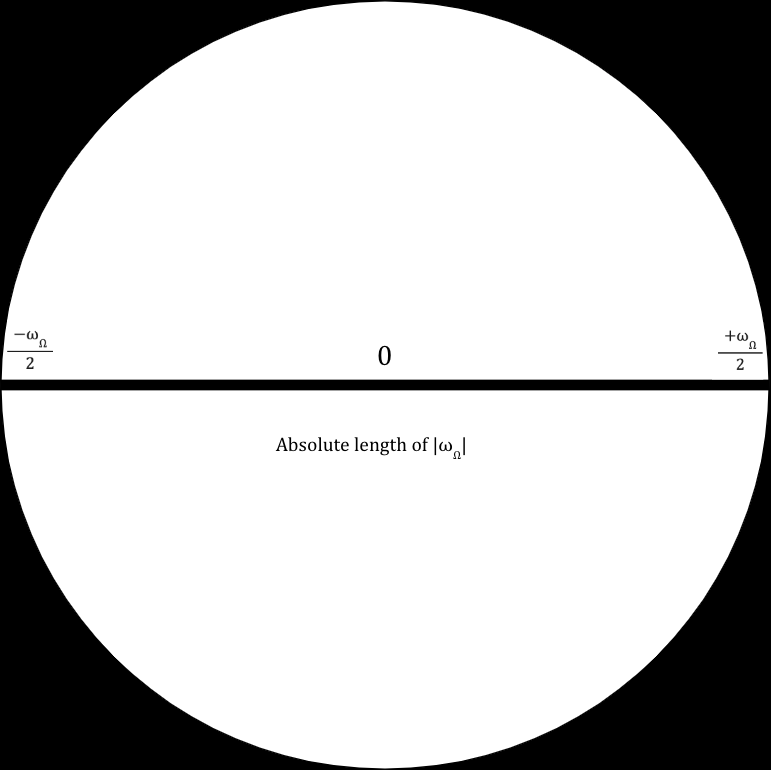
\includegraphics[width=1\linewidth]{Screenshot 2026-03-18 at 02.08.13.png}
    \caption{The geometric one-dimensional continuum $\mathbb{R}_\Omega^1$. 
    Its absolute length is $|\omega_\Omega|$, bounded by the upper bound property. We use ``+'' and ``-'' just to denote relative position to the origin, they aren't intrinsically signed as this is geometric space. Beyond this one dimensional continuum, actuality collapses into infinity.}
    \label{fig:placeholder}
\end{figure}

This distinction between algebraic and geometric $\mathbb{R}_\Omega$ is 
essential before extending to two dimensions. The geometric plane derived 
from $\mathbb{R}_\Omega^1$ is not simply two copies of the algebraic 
$\mathbb{R}_\Omega$ arranged as axes: as one might initially assume.

\subsection{Introduction to $\mathbb{R}_\Omega^2$}

One might expect that two-dimensional geometric space derived from 
$\mathbb{R}_\Omega^1$ is simply the algebraic $\mathbb{R}_\Omega$ extended 
with a second axis, giving a standard $x$-$y$ coordinate plane where both axes 
run from $-\omega_\Omega$ to $+\omega_\Omega$.

\begin{figure}[H]
    \centering
    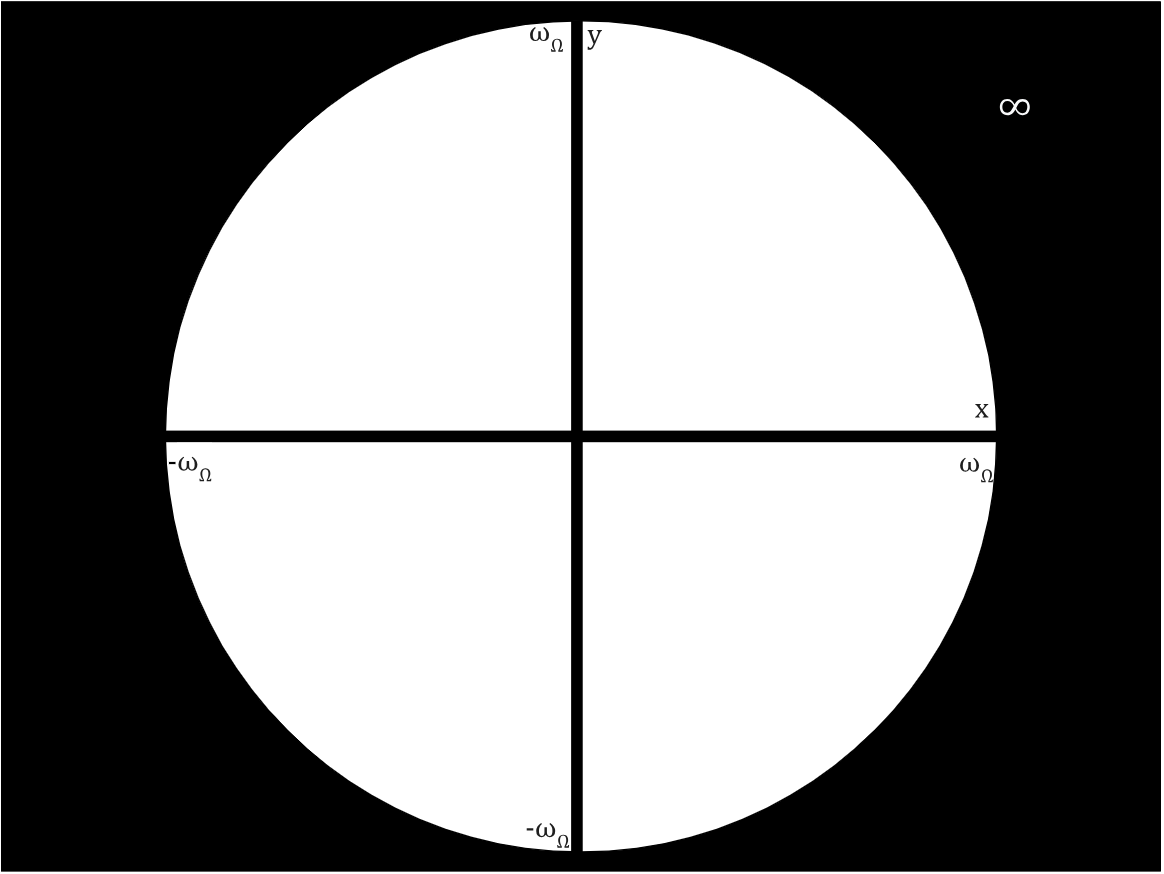
\includegraphics[width=1\linewidth]{Screenshot 2026-03-18 at 02.56.40.png}
    \caption{The naive interpretation: $\mathbb{R}_\Omega^2$ as simply 
    $\mathbb{R}_\Omega$ with an extra axis. This is the algebraic coordinate 
    system used in calculus, but it is not the geometric plane.}
    \label{fig:naive-2d}
\end{figure}

This algebraic coordinate system is useful: it is exactly what is used in 
Chapter 10 for calculus. But it is not the same as the \textit{geometric} $\mathbb{R}_\Omega^2$. Unlike the algebraic 
plane, the geometric plane is subject to the bound property in both 
dimensions simultaneously. That is because the bound property does not merely restrict 
length: it is an \textbf{absolute} property, which means that it restricts \textit{all} measurable geometrical quantities. Since 
area is a product of two lengths, its collapse threshold differs from the 
one-dimensional case.
\\For a square of side length $s$ to enclose \textit{actual} area, we require:
$$s^2 \geq \varepsilon_\Omega \quad \Rightarrow \quad s \geq \sqrt{\varepsilon_\Omega}$$
\\Similarly, for the plane itself to have a finite upper bound on area:
$$s^2 \leq \omega_\Omega \quad \Rightarrow \quad s \leq \sqrt{\omega_\Omega}$$
\\The consequences of this are readily apparent, as it makes it so the geometric plane of $\mathbb{R}_\Omega^2$ is therefore bounded in length as being a finite plane of total area $|\omega_\Omega|$ (visualized in Figure 15), comprising of an infinite amount of absolute infinitesimal cells of length $\sqrt{\varepsilon_\Omega}$ (as visualized 
in Figure 16). Its structure has two immediate 
consequences for how $\mathbb{R}_\Omega^1$ relates to $\mathbb{R}_\Omega^2$:

\begin{itemize}
\item \textbf{Lower bound:} The smallest possible length in 
$\mathbb{R}_\Omega^2$ is $\sqrt{\varepsilon_\Omega}$, since this is 
the minimum side length required to enclose actual area $\varepsilon_\Omega$. 
The absolute infinitesimal $\varepsilon_\Omega$ itself exists in 
$\mathbb{R}_\Omega^2$ only as an \textit{area}, and  not as a length. 
Points in $\mathbb{R}_\Omega^1$ separated by less than $\sqrt{\varepsilon_\Omega}$ 
cannot occupy distinct positions in $\mathbb{R}_\Omega^2$.

\item \textbf{Upper bound:} The largest possible length in 
$\mathbb{R}_\Omega^2$ is $\sqrt{\omega_\Omega}$, since this is the 
maximum side length before area exceeds $\omega_\Omega$ and actuality 
collapses. The absolute hyperfinite $\omega_\Omega$ exists in 
$\mathbb{R}_\Omega^2$ only as an \textit{area}, and not as a length. 
Points beyond $\sqrt{\omega_\Omega}$ in length do not exist in 
$\mathbb{R}_\Omega^2$ at all.
\end{itemize}

\begin{figure}[H]
    \centering
    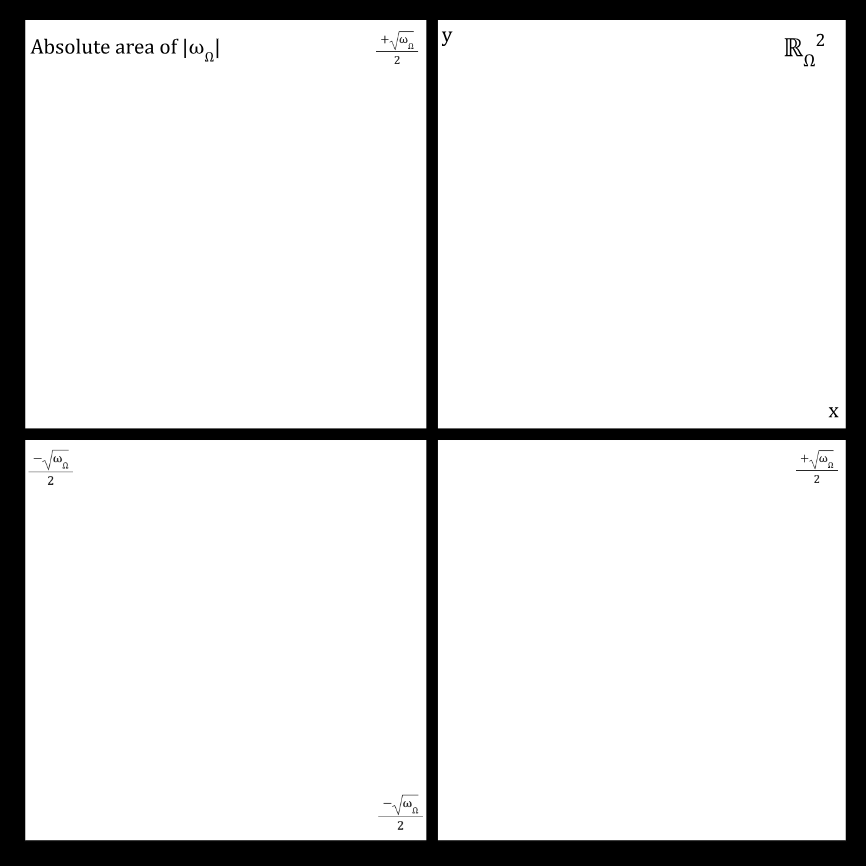
\includegraphics[width=0.7\linewidth]{Screenshot 2026-03-18 at 03.03.34.png}
    \caption{The geometric $\mathbb{R}_\Omega^2$ at the hyperfinite scale, which is a bounded plane of total 
    area $|\omega_\Omega|$. (The labeling of the axes are purely arbitrary, as we chose to define the origin at the center of this plane, and positive and negative directions relative to this origin. In truth, the lengths are actually unsigned).}
    \label{fig:geometric-2d}
\end{figure}

\begin{figure}[H]
    \centering
    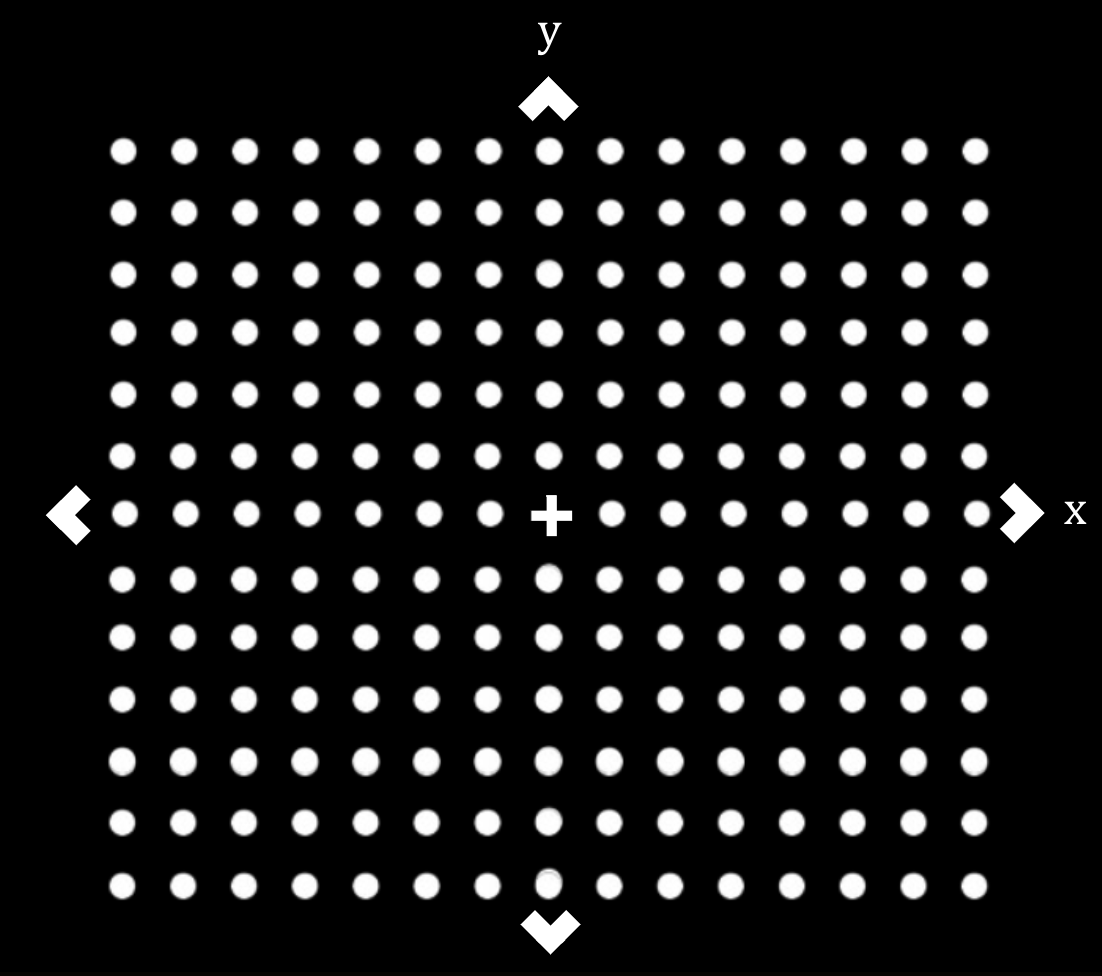
\includegraphics[width=0.9\linewidth]{download.png}
    \caption{2-D space at the absolute infinitesimal scale: a discrete grid in which each 
    point occupies a unique cell, with spacing $\sqrt{\varepsilon_\Omega}$ 
    along both axes. Points between these cells do not exist as distinct actual positions in $\mathbb{R}_\Omega^2$}
    \label{fig:discrete-grid}
\end{figure}

This means that the geometric structure of $\mathbb{R}_\Omega^1$ does 
not embed into $\mathbb{R}_\Omega^2$. In $\mathbb{R}_\Omega$, one can 
define a set of points at distances $\varepsilon_\Omega \leq x \leq 
\sqrt{\varepsilon_\Omega}$ from an origin (such as $(x+\varepsilon_\Omega)$): these are valid, distinct 
positions on the one-dimensional geometric $\mathbb{R}_\Omega^1$. In 
$\mathbb{R}_\Omega^2$, no such distinct positions exist: any two points 
separated by less than $\sqrt{\varepsilon_\Omega}$ collapse to the same actual location. The finer resolution of one-dimensional space is simply 
unavailable in two dimensions.
\\This is a fundamental departure from continuous geometry, where $\mathbb{R}$ 
embeds naturally into $\mathbb{R}^2$ by identifying it with the $x$-axis. In 
$\mathbb{R}_\Omega^1$, the discreteness of space prevents this embedding. Essentially, this means that the 
algebraic and geometric structures of $\mathbb{R}_\Omega^1$ and $\mathbb{R}_\Omega^2$ are genuinely distinct, as one dimensional length in $\mathbb{R}^2_\Omega$ does not possess the same elements as one dimensional length in $\mathbb{R}_\Omega^1$, as $\varepsilon_\Omega$ and $\omega_\Omega$ do not exist as lengths in $\mathbb{R}_\Omega^2$, while they do in $\mathbb{R}_\Omega^1$.
\\It is worth noting, however, that $\mathbb{R}^2 \subseteq \mathbb{R}_\Omega^2$. 
The real plane sits inside the geometric absolute hyper-real plane as a 
continuous sub-region: if one were to zoom into any point on Figure 15, they'd eventually arrive to a $\mathbb{R}^2$ monad.

\subsubsection{Atomic Geometry in $\mathbb{R}_\Omega^2$}

Since $\sqrt{\varepsilon_\Omega}$ is the minimum actual length in 
$\mathbb{R}_\Omega^2$, we refer to geometry at this scale as the 
\textbf{atomic scale}, borrowing from the original Greek meaning of the  
word \textit{atomos}, meaning indivisible. At this scale, no finer geometric 
structure exists.
\\At the atomic scale, $\mathbb{R}_\Omega^2$ does not behave like the 
continuous plane we are accustomed to. Both coordinates must sustain 
actual two-dimensional positions simultaneously, which forces the plane 
to function as a \textbf{discrete grid}\footnote{As seen in Figure 16}: a pixel-like structure in which 
every point occupies a unique cell, with spacing $\sqrt{\varepsilon_\Omega}$ 
in both directions.
\\This is why the $x$-axis cannot retain its one-dimensional resolution 
of $\varepsilon_\Omega$ in two-dimensional space. A point 
$(x + \varepsilon_\Omega,\ 0)$ is a well-defined unique position in 
$\mathbb{R}_\Omega^1$, while in $\mathbb{R}_\Omega^2$ it is not, as no 
unique cell exists for it to occupy, making it physically indistinguishable from
$(x,\ 0)$. Sustaining a distinct two-dimensional position requires 
$\sqrt{\varepsilon_\Omega}$ resolution on both axes simultaneously.
\\The consequence of this is that  \textbf{all geometry in $\mathbb{R}_\Omega^2$ 
is pixelated at the atomic scale}. Any curve, line, or figure, no matter 
how smooth it appears at macroscopic scales - is, at the atomic level, a 
discrete arrangement of grid points. A diagonal line, for instance, cannot 
be truly straight at this scale: it takes on a \textbf{staircase appearance}, 
advancing one grid step horizontally, then one vertically.

\begin{figure}[H]
    \centering
    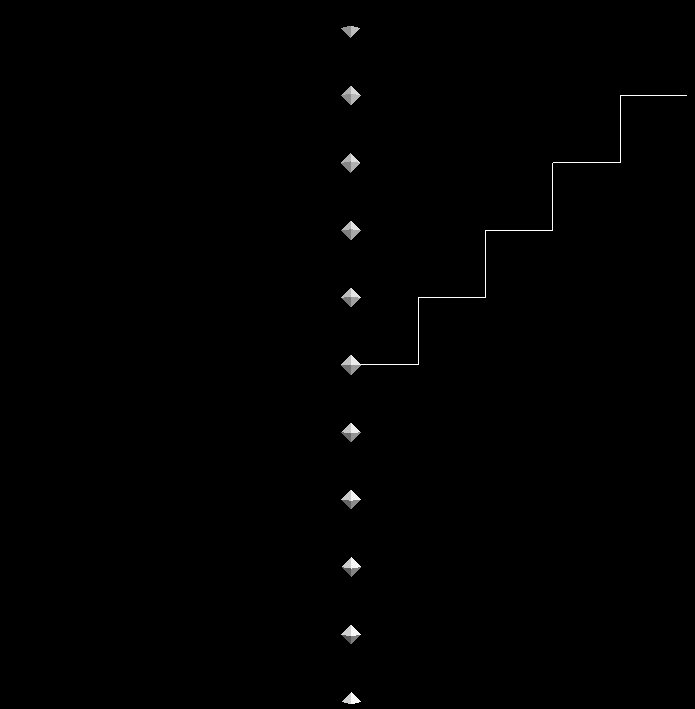
\includegraphics[width=0.6\linewidth]{Screenshot 2026-03-05 at 18.29.25.png}
        \caption{A diagonal line at the atomic scale in $\mathbb{R}_\Omega^2$: 
    a staircase of horizontal and vertical steps of length 
    $\sqrt{\varepsilon_\Omega}$.}
    \label{fig:staircase-line}
\end{figure}

This also explains why $\mathbb{R}^2 \subseteq \mathbb{R}_\Omega^2$: at 
macroscopic scales, the grid spacing $\sqrt{\varepsilon_\Omega}$ is 
imperceptible, and geometry behaves as if space were continuous. The 
discrete structure only becomes apparent at the atomic scale.

\subsubsection{Dimensional Collapse in $\mathbb{R}_\Omega^2$}

Consider a unit square of side length 1 and area 1. In standard Euclidean 
space $\mathbb{R}^2$, the following square resembles the following figure:

\begin{figure}[H]
    \centering
    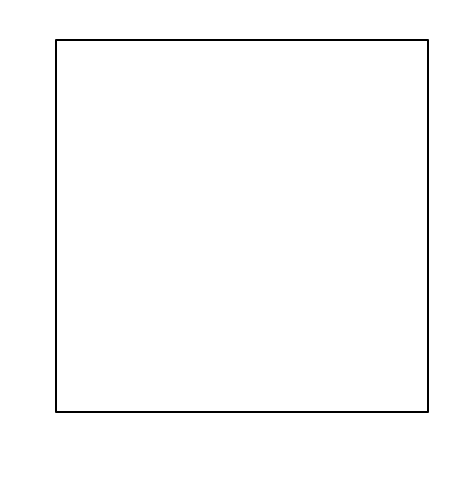
\includegraphics[width=0.3\linewidth]{Screenshot 2026-03-18 at 03.38.15.png}
    \caption{A unit square with side length 1 and area 1.}
    \label{fig:unit-square}
\end{figure}

In $\mathbb{R}^2$, we can scale this square freely and proportionally:

\begin{center}
\begin{tabular}{l c c}
\textbf{Measurement} & \textbf{Scale by 3} & \textbf{Scale by $\frac{1}{10}$} \\
\hline
Edge length & $3$ units & $0.1$ units \\
Perimeter & $12$ units & $0.4$ units \\
Area & $9$ units$^2$ & $0.01$ units$^2$
\end{tabular}
\end{center}

However, in $\mathbb{R}_\Omega^2$, scale invariance breaks down. You can no longer scale freely, as scaling a square below the atomic threshold $\sqrt{\varepsilon_\Omega}$ causes it to lose 
its physical geometry entirely. At side length $\varepsilon_\Omega$ (which isn't a properly defined length $\mathbb{R}_\Omega^2$), a square would have an area of:
$$\varepsilon_\Omega^2 < \varepsilon_\Omega \implies \varepsilon_\Omega^2 = 0$$ Which is zero-equivalent by the lower bound property. This means that the square can no longer enclose actual area, and we describe the square as collapsing to a point.

\begin{figure}[H]
    \centering
    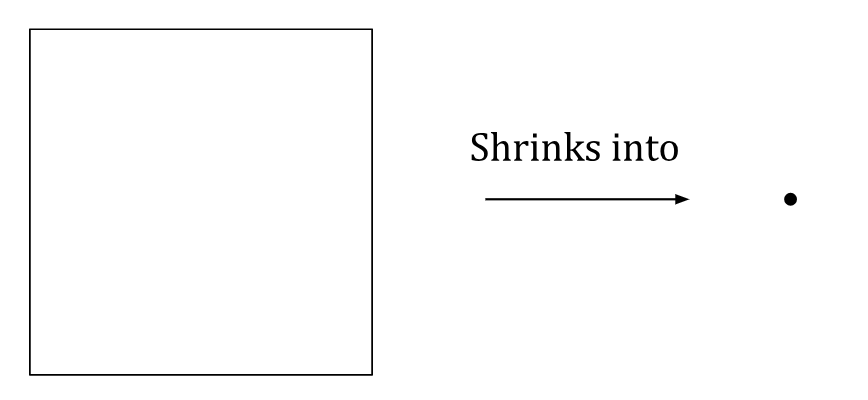
\includegraphics[width=0.5\linewidth]{Screenshot 2026-03-18 at 04.59.38.png}
    \caption{The unit square scaled to side length $\varepsilon_\Omega$. 
    Its area is $\varepsilon_\Omega^2 < \varepsilon_\Omega$, which is 
    zero-equivalent. The square has collapsed to a point.}
    \label{fig:square-collapsed-point}
\end{figure}

If we were to re-measure it, we'd find it would have the following measurements in $\mathbb{R}_\Omega^2$:
\begin{center}
\begin{tabular}{l c c}
\textbf{Measurement} & \textbf{Original} & \textbf{Scaled to $\varepsilon_\Omega$} \\
\hline
Edge length & $1$ unit & 0 ($\varepsilon_\Omega$ in $\mathbb{R}_\Omega^1$) \\
Perimeter & $4$ units & 0 ($\varepsilon_\Omega$ in $\mathbb{R}_\Omega^1$) \\
Area & $1$ unit$^2$ & $0$
\end{tabular}
\end{center}

This collapse is not unique to squares. \textbf{Any} two-dimensional figure, whether it be a square, triangle or circle, or any other arbitrary shape, when scaled below the 
atomic threshold $\sqrt{\varepsilon_\Omega}$ collapses to the same result: 
a single point.

\begin{figure}[H]
    \centering
    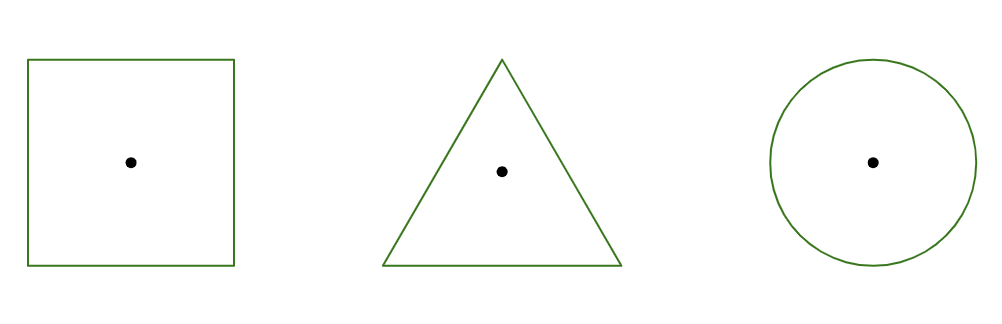
\includegraphics[width=0.5\linewidth]{Screenshot 2026-03-18 at 06.50.23.png}
    \caption{A circle, square, and equilateral triangle, each scaled below 
    $\sqrt{\varepsilon_\Omega}$. Physically, all three are identical: a single 
    point. We draw in green what the dots used to physically resemble before their dimensional collapse}.
    \label{fig:indistinguishable}
\end{figure}At this scale, the distinguishing features of these figures: their 
shapes, their angles, their defining geometries, have vanished in 
actuality. A collapsed circle is physically identical to a collapsed square 
or a collapsed triangle. All appear as the same structureless point, with this collapsed square no longer remaining a square in any physical sense. What remains is a geometric ghost: 
the remnant of a figure that once was, stripped of all distinguishing 
physical features.
\\Yet to conclude that the square is truly \textit{gone}, that its 
identity has been erased, would be hasty. For while actuality collapses 
at this scale, \textbf{virtuality} persists, preserving structural information beyond the scale of actuality. The point is not a square by 
form, but it remains a square \textbf{by nature}. And that is where 
\textbf{geometric data} enters the framework\footnote{This notation of illustrating a figure in green is what is known as the \textbf{virtual} geometrical notation, which will be covered in the next section.}.

\subsection{Geometric Data: Virtual Identity in Physical Collapse}

In the previous section, we witnessed the dimensional collapse of a square 
below the atomic threshold $\sqrt{\varepsilon_\Omega}$: its area became 
zero-equivalent, and the figure collapsed to a point. 
\\\\However, the collapsed point is not mere nothingness. It is a 
\textit{distinct} collapsed structure, carrying information that 
differentiates it from other collapsed figures. A point that was once a 
square differs fundamentally from a point that was once a circle, or a 
triangle, even though physically, at this scale, they are 
indistinguishable.
\\This persistence of structural information despite physical collapse is 
what is referred to as \textbf{geometric data} in this framework. It is 
the third manifestation of mathematical data in this theory, alongside 
sub-infinitesimal data and specific infinite data. Where sub-infinitesimal 
data preserves numerical magnitudes when they fall below the lower bound, 
geometric data preserves \textit{structural} identity when physical geometry 
collapses. Put more simply, while sub-infinitesimal data preserves 
``how much?'' (what magnitude was lost),  geometric data preserves 
``what kind?'' (what structure was lost). A zero with sub-infinitesimal 
data ``remembers'' being $0.5\varepsilon_\Omega$; a point with geometric 
data ``remembers'' being a square.
\\The distinction is crucial: sub-infinitesimal data operates on 
magnitudes - individual lengths and areas that have become 
zero-equivalent. Geometric data operates on \textbf{structures}. Geometric data focuses on the relationships \textit{between} those magnitudes, the configuration of vertices 
and edges that define a figure's identity. When a square collapses to a 
point, each individual edge length carries sub-infinitesimal data about 
its edge geometries virtually, but it is geometric data that preserves 
the fact that those edges formed a square, not a circle or a triangle. 
Critically, the two forms of metadata nest: geometric data encompasses 
sub-infinitesimal data as a component, since preserving a figure's 
structure necessarily includes preserving the specific zero-equivalent 
magnitudes of its collapsed edges and area.
\\Even when every physical feature is lost, the structural identity 
persists virtually through geometric data. This allows collapsed 
structures to retain mathematical behavior despite physical 
nonexistence. A collapsed square can still be scaled or transformed as 
a square, because its geometric data encodes square-specific 
transformations and responses. The physical form may be gone, but the 
virtual identity remains.

\subsubsection{Recovery of Structure Through Geometric Data}

The validation of geometric data lies in its capacity to enable structural recovery. A figure whose geometry collapsed can be scaled back to finite size, recovering not merely \textit{some} of the geometric object, but the \textit{entire} specific figure it originally was. This recovery is algebraically instantaneous and structurally precise.
For example, let us consider a square in $\mathbb{R}_\Omega^2$ which was scaled down to a dot by scaling the structure's edge lengths to $\varepsilon_\Omega$.

\begin{figure} [H]
    \centering
    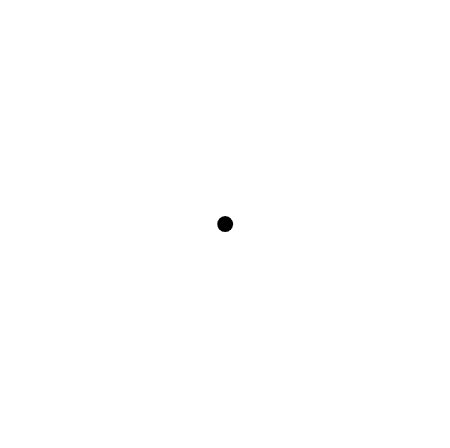
\includegraphics[width=0.2\linewidth]{Screenshot 2026-03-18 at 06.59.05.png}
    \caption{A physical dot representing a square shrunk down to edge length $\varepsilon_\Omega$}
    \label{fig:placeholder}
\end{figure}
\begin{center}
\begin{tabular}{l c c c}
\textbf{Measurement} & \textbf{Original} & \textbf{In $\mathbb{R}_\Omega^1$} & \textbf{In $\mathbb{R}_\Omega^2$} \\
\hline
Edge length & $1$ unit & $\varepsilon_\Omega$ & 0 \\
Perimeter & $4$ units & $\varepsilon_\Omega$ & 0 \\
Area & $1$ unit$^2$ & 0 & $0$ \\
Geometric status & Square & Line segment & Point \\
\end{tabular}
\end{center}

The scaling down to $\varepsilon_\Omega$ has caused the square to collapse to a dot. However, despite the physical collapse, the identity of the square \textbf{persists virtually} even as a dot - which makes it so when you consider scaling this dot back up to its original scale, it will recover its square shape, and will \textbf{not remain a dot or become a line of length 1}. 

\begin{figure} [H]
    \centering
    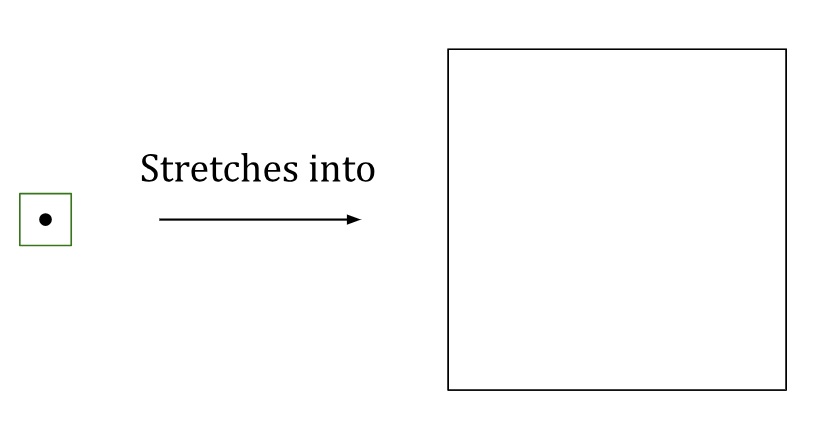
\includegraphics[width=0.75\linewidth]{Screenshot 2026-03-18 at 07.12.16.png}
    \caption{Recovery of a collapsed square through scaling. Geometric data preserved the structural identity through the collapse, enabling precise reconstruction.}
    \label{fig:placeholder}
\end{figure}


\subsubsection*{Why recovery works:}

Recovery succeeds because geometric data is \textit{active}, not passive. It is not merely a label or classification, it is an encoding of behavioral rules. When we scale a collapsed square, geometric data works as a code, instructing the operation: ``These two endpoint dots represent opposite corners of a square. When scaled, generate four edges of equal length at right angles connecting these and two intermediate vertices.''
\\An arbitrarily chosen point has no such instructions. Scaling it does nothing. But a point segment with square-geometric-data \textit{knows} to unfold into a square. The data encodes the transformation rules necessary for recovery.
\\This is the power of virtuality in $\mathbb{R}_\Omega^2$. Physical features may vanish, but virtual instructions persist, enabling not just memory of what was lost, but active reconstruction when conditions permit.

\subsubsection{Geometric data notation}
Although in this specific context it was easy to gather that this point would stretch back into a square (because that \textit{particular} point was \textit{initialized} to possess geometric data through the dimensional collapse of the square), a shorthand notation is still useful, so we sometimes ``visualize'' geometric data.
\\Geometric data notation is color - coded, in which figures illustrated in \textbf{black} are the actual, physical geometry of the figure, while figures illustrated in \textbf{green} are virtual representations of them.
So for example, if we wanted to describe a collapsed circle, square, or triangle, and ``specify'' that these physically identical figures have different virtuality, we usually illustrate the physical geometry \textit{inside} the virtual representation, like so: 

\begin{figure} [H]
    \centering
    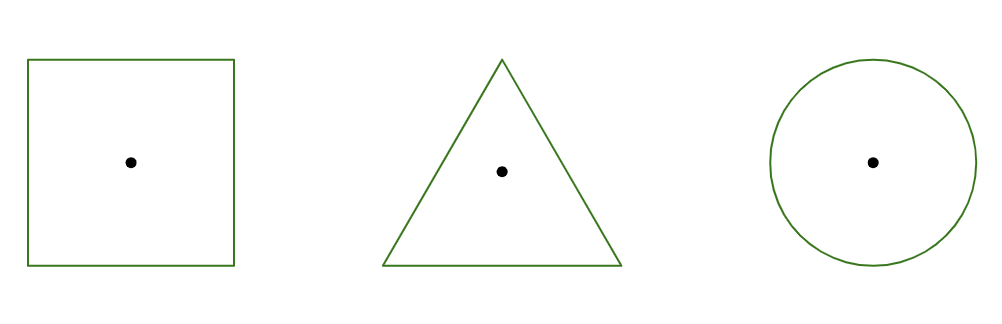
\includegraphics[width=0.5\linewidth]{Screenshot 2026-03-18 at 06.50.23.png}
    \caption{Physical and virtual geometry notation of three figures}
    \label{fig:placeholder}
\end{figure}

\subsubsection*{Important Conceptual Note:}

In $\mathbb{R}_\Omega^2$, these virtual illustrations of figures aren't \textit{literal}, meaning these visualizations do not ``physically'' exist on some continuously defined virtual plane. It is more accurate to define virtually purely as being \textit{code} which these points inherit from dimensional collapse. This will be elaborated upon in Chapter 9. 
 
\subsubsection{Traditional Zero vs. Zero-Equivalent}

Before proceeding from geometrical recovery, we must distinguish between two fundamentally different ways a figure can collapse to a point: reduction below atomic thresholds versus multiplication by traditional zero.

\subsubsection*{Method 1: Reduction below atomic thresholds (zero-equivalent)}

Consider a line segment of length $10\varepsilon_\Omega$ in $\mathbb{R}_\Omega^1$. If we scale it down by a factor of 20:
$$\text{New length: } \frac{10\varepsilon_\Omega}{20} = 0.5\varepsilon_\Omega < \varepsilon_\Omega$$
\\This length is below the one-dimensional atomic threshold, and it becomes zero-equivalent, making it so the line collapses to a point. However, this point carries geometric data: it ``remembers'' having been a line segment of length $10\varepsilon_\Omega$. Crucially, this point is \textbf{recoverable}. Scaling upward by any finite factor in $\mathbb{R}_\Omega^1$ can restore the line:
$$\text{Scaled by 20: } 0_{[0.5\varepsilon_\Omega]} \times 20 = 10\varepsilon_\Omega$$
\\The line reforms. Recovery is straightforward.

\subsubsection*{Method 2: Multiplication by traditional zero}

Now take the same line segment of length $10\varepsilon_\Omega$ and multiply by traditional zero:
$$10\varepsilon_\Omega \times 0_{[0]} = 0_{[0]}$$The result is also a point. This point \textit{still carries geometric data}, as it virtually remembers being a line segment. However, there is a critical difference: this point is \textbf{not recoverable by standard scaling}.
\\Multiplying this point by any finite element of $\mathbb{R}_\Omega^1$ does nothing:
$$0_{[0]} \times k = 0_{[0]} \quad \text{for any } k \in \mathbb{R}_\Omega^1$$
\\The point remains unchanged. No finite scaling factor can restore the line. The traditional zero's multiplicative annihilator property persists: it ``locks'' the structure at zero. The only method this point could be recovered is by multiplying it an appropriate specific infinite data, otherwise the figure remains unrecoverable. \footnote{This will be covered in the following chapter.}

\subsubsection*{Why this distinction matters}

The key insight is this: a point created by multiplication by traditional zero is \textbf{resistant to finite scaling}. No matter what finite number you multiply it by, it remains a point. This property of annihilation of scale factors, is precisely what enables the geometric definition of division by zero through a mechanism we call \textit{geometric encoding into a physical structure}, which is when we encode the virtual geometry of one figure into the physical structure of another.
\\Doing this is useful as it allows us to create objects that behave counterintuitively under scaling. This encoding, made possible by the distinction between zero-equivalent collapse and traditional zero multiplication, is the foundation for defining $\frac{1}{0}$.

\subsection{Geometric Encoding into a Physical Structure}

So far, we have established that geometric data preserves structural identity when physical geometry collapses. A point can ``remember'' being a square through virtual preservation. Now we introduce a more radical concept: \textbf{geometric encoding} - where the virtual geometry of one figure is deliberately imposed onto the physical structure of a different figure. This allows us to create geometrical objects with counterintuitive behavior, enabling the mechanism by which we define division by zero.

\subsubsection{Conceptual Illustration: A Triangle That Is a Square}

Consider an equilateral triangle in $\mathbb{R}^2$ with measurable edge lengths and area:

\begin{figure}[H]
    \centering
    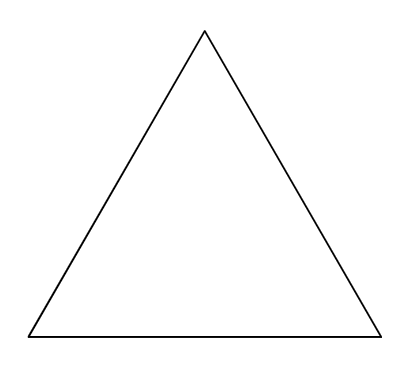
\includegraphics[width=0.2\linewidth]{Screenshot 2026-02-11 at 05.27.13.png}
    \caption{A triangle with actual geometry: three sides, angles of 60°, measurable area.}
    \label{fig:triangle-actual}
\end{figure}

By every physical measurement, this is a triangle. Yet suppose that when we scale this figure, by multiplying any of its dimensions by any factor $n\neq1$. For some inexplicable reason, it does not behave as a triangle. Instead, it transforms into a square:

\begin{figure}[H]
    \centering
    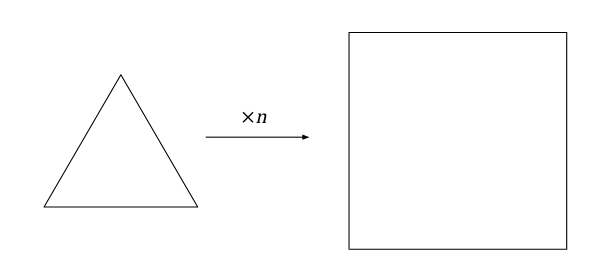
\includegraphics[width=0.6\linewidth]{Screenshot 2026-02-11 at 05.27.22.png}
    \caption{Scaling the triangle produces a square, not a larger triangle.}
    \label{fig:triangle-to-square}
\end{figure}

This is absurd by standard geometric reasoning. How can a triangle become a square through simple scaling?
\\The answer lies in the triangle's \textbf{virtuality}. This figure \textit{physically} appears to be a triangle but it is \textit{virtually} defined as being a square. This makes it so when an operation is performed, such as scaling, rotation or any kind of transformation, the virtual geometry governs the response. The triangle behaves as a square because it \textit{is} a square virtually, even though it appears as a triangle physically.

\subsubsection*{How could this occur?}

One explanation: the geometric space this square inhabited underwent exotic dimensional behavior at a particular scale, forcing the square to physically collapse into a triangle configuration while retaining square-virtual-geometry. The collapse altered physical appearance but preserved virtual identity through geometric data.

\subsubsection*{Important caveat:}
This triangle-square example is a \textit{conceptual illustration only}. 
In practice, a square collapsing in $\mathbb{R}_\Omega^2$ does not become 
a triangle: it collapses directly to a point, as established in the 
previous section. However, the core idea of having \textbf{physical structure 
carrying the virtual geometry of a different structure} is not merely 
conceptual. It is actually \textbf{essential} to defining curvature and division by zero, 
as will be seen in the following chapters.

\subsubsection{Application: A Line That Is a Dot}

While we may never encounter a finite-scale square behaving as a triangle, we \textit{do} encounter atomic line segments that carry the virtual geometry of points.
\\Consider a line segment of physical length $\varepsilon_\Omega$:

\begin{figure}[H]
    \centering
    
\includegraphics[width=0.4\linewidth]{Screenshot 2026-03-19 at 04.00.14.png}
    \caption{Physical geometry: line segment of length $\sqrt{\varepsilon_\Omega}$. Virtuality: zero-dimensional point.}
    \label{fig:line-is-dot}
\end{figure}

Physically, this is a line segment of length $\sqrt{\varepsilon_\Omega}$ \footnote{In $\mathbb{R}_\Omega^1$ this line segment can be subdivided hyper-finitely, while in $\mathbb{R}_\Omega^2$ it would collapse into zero}. But suppose this line carries the virtual geometry of a traditional zero-dimensional point. Specifically, a point created by multiplication by $0_{[0]}$ as discussed in the previous section.
\\This virtual point-geometry imposes \textbf{scaling resistance}. Because zero is a multiplicative annihilator, any scaling applied to this figure produces no change. When we scale by a factor $k$ (where $k > 1$):

\begin{align*}
\text{Scaling upward:} & \quad 0 \times k = 0 \\
\text{Scaling downward:} & \quad 0 \times \frac{1}{k} = 0
\end{align*}
\\Virtually, the operation behaves as multiplication by zero. The scale factor is annihilated. But because the structure is \textit{physically} a line of length $\sqrt{\varepsilon_\Omega}$, what we observe is a line that does not stretch or shrink at all when scaled, remaining locked at $\sqrt{\varepsilon_\Omega}$ regardless of the scaling factor applied.
\\The result: a line segment that behaves as a zero-dimensional point would, exhibiting complete inertness under scaling operations. The virtual point-geometry overrides what would normally be a change in length, rendering the physical line unchangeable.
\\This property of having a line that resists scaling as if it were a point, is in truth the \textbf{foundational mechanism} by which curvature is defined in this 
number system. Why a line acquires this point-like virtual geometry, 
and how it connects to division by zero, will be established in the 
following chapter, which is where we finally arrive at this theory's 
climax: \textbf{defining division by zero}.

\newpage

\section{Chapter 8 - Circles and Curvature $\mathbb{R}_\Omega^2$} 

This is the long awaited chapter in which we shall finally describe and define 
division by zero. It is true that this paper has taken a far more circuitous 
route of defining division by zero - instead of defining division by zero 
directly, we first constructed an entire number system in which many concepts 
have been introduced and discussed. Most notably: the concept of mathematical 
data, the absolute hyper-reals, and absolute hyper-real geometry. Although 
lengthy, all of this was imperative to establish, as it is all necessary in 
order to understand and define the \textbf{full} definition of division by 
zero - not just the actual identity of $\frac{1}{0} = \infty$ . The way in which we define traditional division by zero (the 
one with its annihilator property) is achieved \textit{through geometry}.\\\\
As strange as this may sound, it is true. Division by zero is defined as a 
\textit{specific infinite data} of infinity: a sort of ``code'' which enables 
and defines curvature in this number system. In this framework, division by 
zero \textbf{isn't} a number to be declared. It is not some unique, made-up 
value. Its actual value is simply infinity. Virtually, however, it describes a 
\textbf{geometric property} - specifically, it is understood as the virtual 
geometry, or ``code'', which underlies the behaviour of circles in 
$\mathbb{R}_\Omega^2$.\\\\
This may not make a great deal of sense at face value, but that is precisely 
what this chapter shall address. Although we have defined geometry in 
$\mathbb{R}_\Omega^2$, including the concept of dimensional collapse at certain 
thresholds, circles have not yet been properly treated, despite being among the 
most fundamental figures in geometry. The reason for this omission is that, 
despite their apparent simplicity, circles become something of an impossibility 
in $\mathbb{R}_\Omega^2$, because of the fact that \textbf{circles require continuous curvature, but 
$\mathbb{R}_\Omega^2$ is \textit{discrete}.}


\subsection{The Problem with Circles in $\mathbb{R}_\Omega^2$}

In traditional Euclidean geometry, circles are purely continuous figures. Unlike polygons, which are piecewise linear (constructed from discrete edges 
joined at vertices). Circles are a single unbroken curve with no straight 
segments, in which every point on a circle's boundary lies on a smooth, 
continuously curving path.\\\\
This continuity is fundamental to a circle's geometric properties, as it 
enables the circle to behave differently from its visually similar yet discrete 
counterpart - regular polygons. For example, a tangent line to a circle touches 
it at exactly one point, whereas a tangent to a polygon's edge coincides with 
that entire edge. This distinction reflects the circle's essential nature: it 
has no corners, no flat sections, only uniform curvature at every point along 
its perimeter. The standard definition captures this precisely: a circle is the 
set of all points in a plane equidistant from a fixed center point. No polygon, 
regardless of how many sides it possesses, can satisfy this definition exactly 
in Euclidean space. As a regular polygon's side count increases, it approximates 
a circle more closely, but the approximation remains asymptotic: approaching, 
but never reaching, true circularity.

\begin{figure}[H]
    \centering
    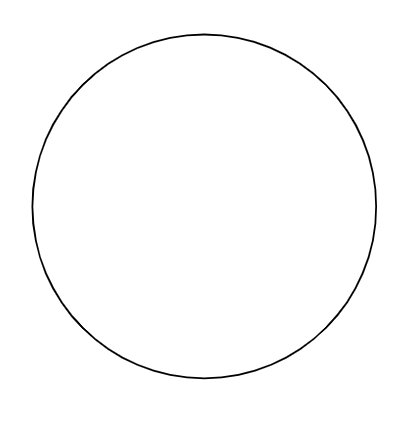
\includegraphics[width=0.3\linewidth]{Screenshot 2026-02-12 at 02.49.00.png}
    \caption{A circle}
    \label{fig:circle-finite-scale}
\end{figure}

However, in $\mathbb{R}_\Omega^2$, this is a different story. Although the 
absolute hyper-reals are technically a superset of the reals, which are defined 
as being absolutely continuous, the absolute hyper-reals are \textit{not} 
absolutely continuous. They have a minimal incrementing element - the 
\textit{absolute infinitesimal} - which makes curvature and smoothness 
impossible at a certain scale, because space is \textit{discrete}, constructed 
in increments of $\sqrt{\varepsilon_\Omega}$. Therefore, a circle can no longer 
\textit{be} a smooth curve in $\mathbb{R}_\Omega^2$; it must instead be 
approximated by discrete points separated by $\sqrt{\varepsilon_\Omega}$ 
intervals.\\However, to conclude that circles are therefore a simple impossibility in 
$\mathbb{R}_\Omega^2$, would be too hasty. Circles \textit{do} exist 
in $\mathbb{R}_\Omega^2$ - it is simply that the way they are defined and 
interpreted differs fundamentally from their standard real-derived definition. 
So much so, in fact, that they exist not as purely physical structures, but as 
\textbf{virtual} ones. To understand why this is, we must first investigate the 
discrete nature of geometry in $\mathbb{R}_\Omega^2$.

\subsubsection{The Discrete Nature of $\mathbb{R}_\Omega^2$}

As was established in Chapter 7, $\mathbb{R}_\Omega^2$ is inherently discrete 
at the atomic scale, incrementing in steps of $\sqrt{\varepsilon_\Omega}$. 
At macroscopic scales however, that is, when viewing any figure within $\mathbb{R}^2$ in $\mathbb{R}^2_\Omega$, this discreteness is imperceptible. 

\begin{figure}[H]
    \centering
    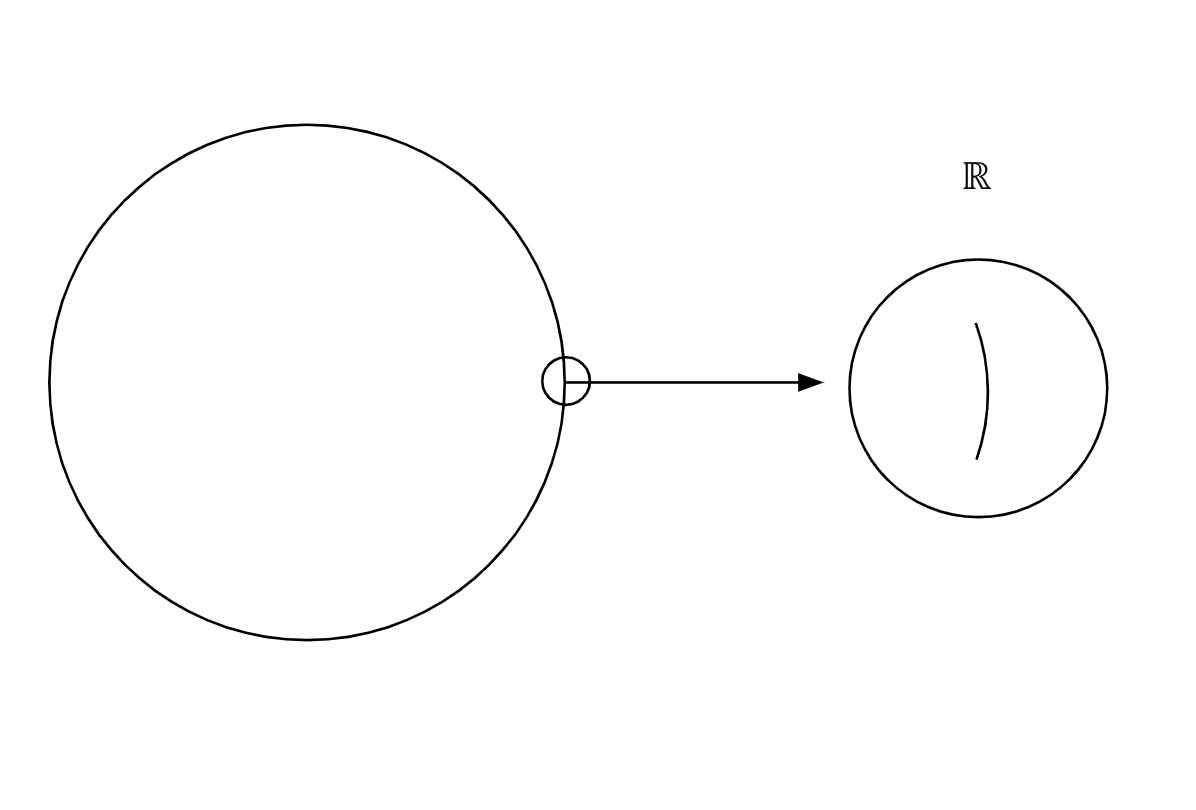
\includegraphics[width=0.5\linewidth]{Screenshot 2026-03-11 at 01.08.05.png}
    \caption{A circle in $\mathbb{R}_\Omega^2$ viewed at macroscopic scale is zoomed in 
    within $\mathbb{R}^2$: the boundary appears smooth and continuously 
    curved. The discrete structure is not visible at this resolution.}
    \label{fig:circle-macro}
\end{figure}

But this apparent smoothness is a macroscopic illusion. Zooming into any point 
on the boundary at the atomic scale reveals the physical reality: the boundary 
is \textbf{locally completely flat}, consisting of discrete horizontal and 
vertical edge segments of length $\sqrt{\varepsilon_\Omega}$, occasionally 
stepping one pixel inward or outward to trace the overall circular path.

\begin{figure}[H]
    \centering
    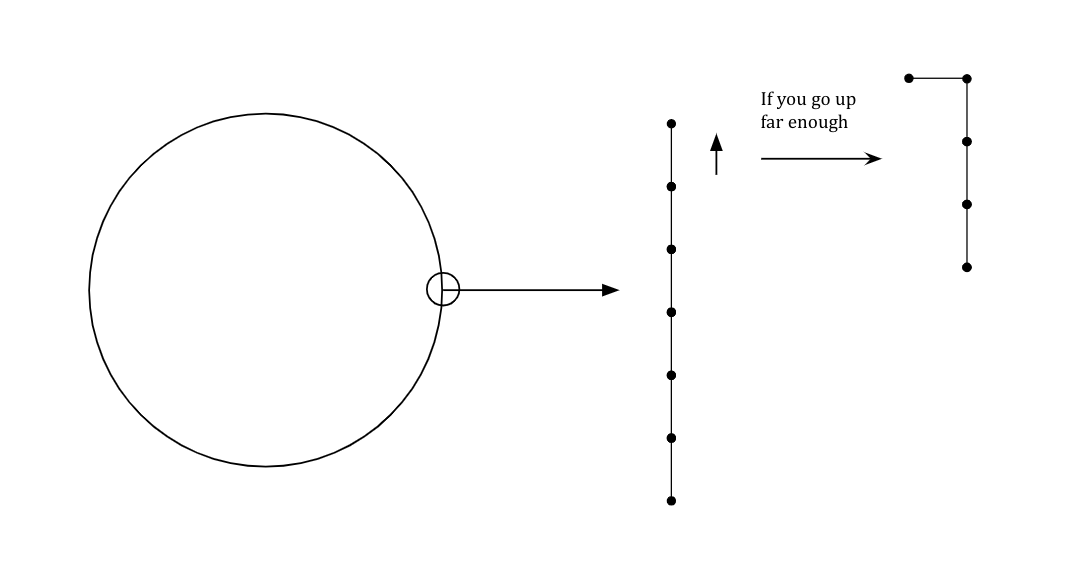
\includegraphics[width=1\linewidth]{Screenshot 2026-03-06 at 16.28.13.png}
    \caption{Zooming into a point on a circle's boundary in 
    $\mathbb{R}_\Omega^2$ reveals a locally flat discrete structure - a 
    staircase of horizontal and vertical steps, deviating by one grid unit 
    at irregular intervals to approximate curvature.}
    \label{fig:circle-local-flat}
\end{figure}

\begin{figure}[H]
    \centering
    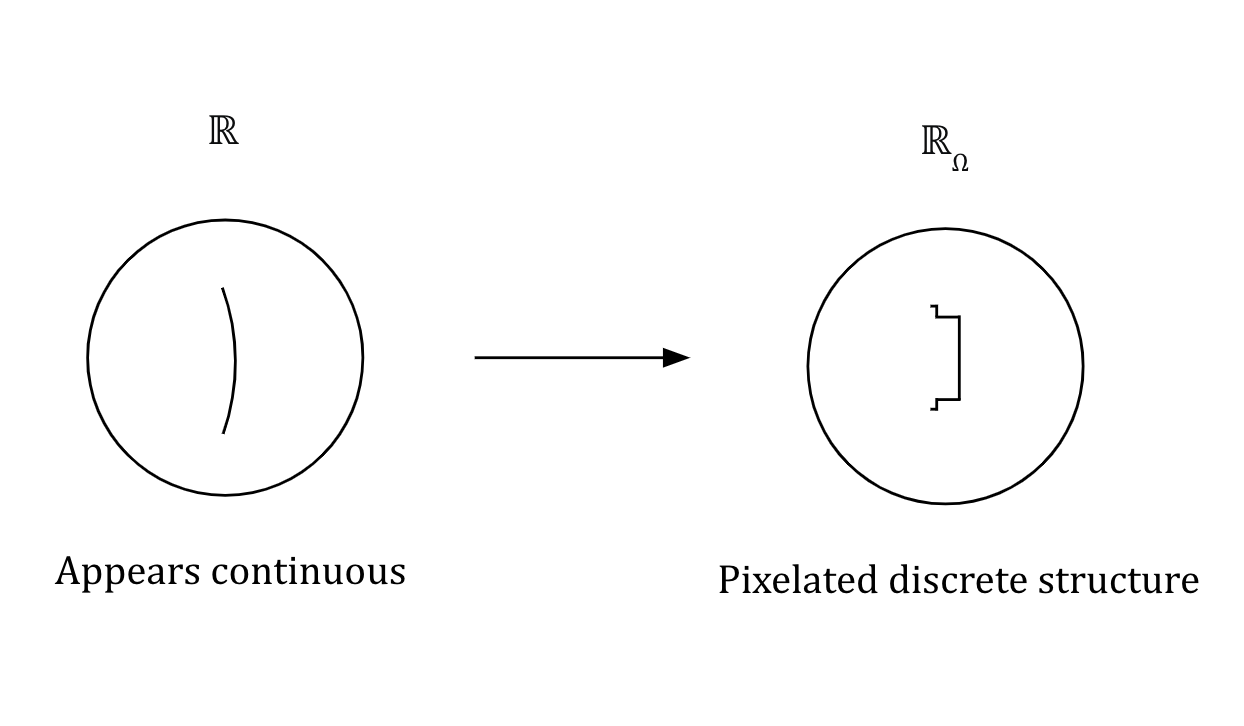
\includegraphics[width=1\linewidth]{Screenshot 2026-03-11 at 01.41.53.png}
    \caption{Local flatness of a circle's boundary in $\mathbb{R}_\Omega^2$ 
    at the atomic scale (left: continuous appearance in $\mathbb{R}$; right: 
    discrete pixelated structure in $\mathbb{R}_\Omega$).}
    \label{fig:circle-pixelated}
\end{figure}

No curve in $\mathbb{R}_\Omega^2$ can possess actual curvature at the atomic 
scale. Curvature is a macroscopic emergent property - at the atomic level, 
every curve is a discrete line, either flat or bent into a staircase.\\\\
A further consequence concerns tangency. In $\mathbb{R}$, a tangent line 
touches a circle at exactly one point. In $\mathbb{R}_\Omega^2$, this is 
physically impossible: the discrete grid forces the tangent line to align with 
multiple adjacent grid points along a flat edge. Single-point tangency cannot 
be achieved (though, as will be discussed in ``the minimum side count for equidistance'', this can be \textit{minimized}).

\begin{figure}[H]
    \centering
    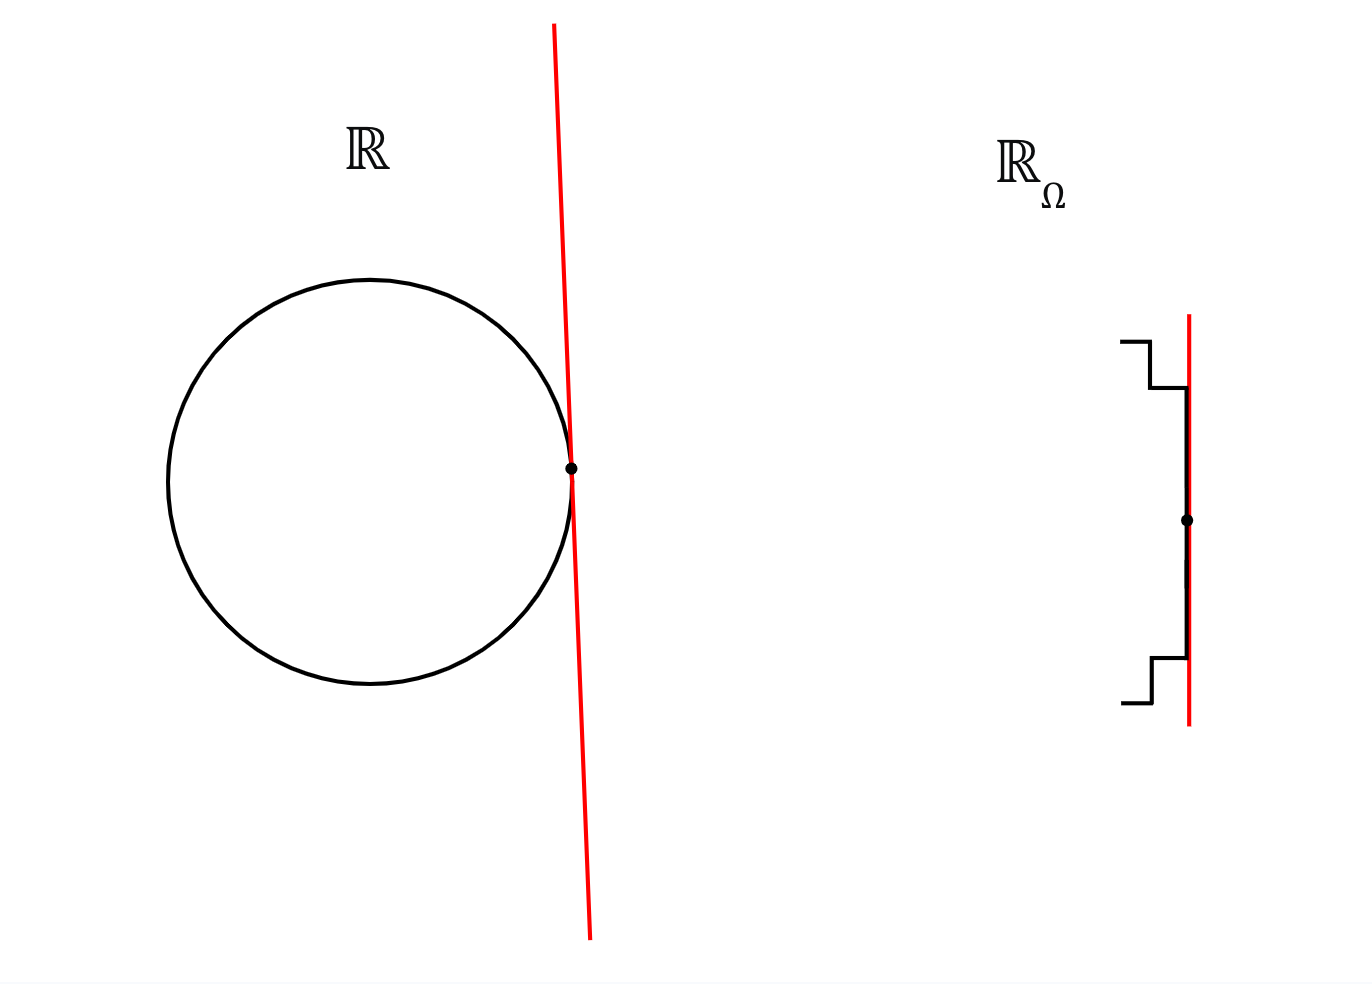
\includegraphics[width=1\linewidth]{Screenshot 2026-03-11 at 02.07.41.png}
    \caption{Tangency in $\mathbb{R}$ (left) versus $\mathbb{R}_\Omega^2$ 
    (right). In $\mathbb{R}$, a tangent line touches the circle at exactly 
    one point. In $\mathbb{R}_\Omega^2$, the discrete boundary forces the 
    tangent to pass through multiple grid points along a flat edge - 
    single-point tangency is physically impossible.}
    \label{fig:tangency-comparison}
\end{figure}

Despite all of this, circularity as a condition does not require smoothness. 
A circle is defined as the set of all points equidistant from a center - and 
this condition is physically achievable in $\mathbb{R}_\Omega^2$, even without 
smoothness or single-point tangency. This requires us to redefine circles not 
as standalone geometric objects, but as a \textit{condition} that regular 
polygons can satisfy once their side count exceeds a threshold.

\subsubsection{Equidistance}

Despite the fact that circles are in a manner, physically impossible, as the requirement of continuous curvature cannot be physically fulfilled in discrete space, we can \textit{still} define a circle as being a figure in which all points are equally spaced apart - as bizarre as that is. It is by defining a circle as being a regular polygon with a large amount of sides.
\\But how can a polygon in discrete space have every point equidistant from the 
center? At first glance, this seems impossible - polygons have vertices and 
edges, and vertices are always farther from the center than edge midpoints.\\\\
The answer lies in a property unique to regular polygons: the \textit{apothem}. 
In $\mathbb{R}_\Omega^2$, all we really need to do is have the ``difference'' between the apothem and circumradius be \textit{zero-equivalent}, meaning, so long as the difference is less than $\sqrt{\varepsilon_\Omega}$ (atomic threshold for 2-D space), this regular polygon technically satisfies the condition for equidistance around a point - making it a circle. To understand why this suffices, we shall discuss exactly what the apothem is, and examine the 
relationship between regular polygons inscribed inside circles and comparing them the 
circumradius to the apothem.\\\\
Consider a regular polygon with $n$ sides inscribed in a circle of radius $r$, 
with two key measurements:
\begin{itemize}
\item \textbf{Circumradius} ($r$): the distance from the center to a vertex 
(the farthest point from the center)
\item \textbf{Apothem} ($a$): the distance from the center to the midpoint of 
an edge (the closest point from the center)
\end{itemize}

The apothem is given by:
$$a = r\cos\left(\frac{\pi}{n}\right)$$

An interactive visualization is available at:
\begin{center}
\url{https://www.geogebra.org/m/kg6juncc}
\end{center}

In the reals, the concept is that as $n$ increases, the apothem approaches 
the circumradius:
$$\lim_{n \to \infty} r\cos\left(\frac{\pi}{n}\right) = r$$For a true circle, every point is equidistant from the center. For a polygon, 
the farthest and closest points differ. But as the side count increases, this 
difference shrinks - and as it approaches infinity, the closest and farthest 
points converge to the same distance, making all points equidistant. In the 
real numbers, this condition is met only ``at infinity'' - approached 
asymptotically but never actually reached. This is, in a way, the essence of 
what a circle is: despite the simplicity of this limit, it captures the 
continuous nature of the figure simply and elegantly.\\\\
The standard hyper-reals take this intuition further. Rather than merely 
approaching infinity, we can substitute a hyperfinite $\omega$ directly into 
the apothem formula:
$$r\cos\left(\frac{\pi}{\omega}\right) \approx r$$
A polygon with a hyperfinite number of sides approximates a circle to within 
infinitesimal precision. However, without the standard part function to round 
off the remaining difference, the apothem-circumradius gap remains nonzero - 
the polygon is infinitesimally close to a circle without actually being 
one.\cite{goldblatt1998hyperreals} The standard part function is 
still required for the figure to \textit{be} a circle:
$$\text{st}\left(r\cos\left(\frac{\pi}{\omega}\right)\right) = r$$ $\mathbb{R}_\Omega^2$ completes what the hyper-reals only approximate. Rather 
than needing a standard part function to close the gap, the gap closes itself. 
We have a lower bound of magnitude, and when the apothem-circumradius difference 
falls below $\sqrt{\varepsilon_\Omega}$ - the 2D atomic threshold - it becomes 
zero-equivalent. At that point, $r$ and $a$ are not approximately equal: they 
are \textit{exactly} equal. A regular polygon with enough sides to bring this 
difference below $\sqrt{\varepsilon_\Omega}$ therefore satisfies the 
equidistance condition exactly - no rounding, no approximation, no standard 
part function required. Circles are no longer unattainable limits. They are 
conditions that polygons \textit{do} satisfy, once their side count exceeds a 
threshold.

\subsubsection{The Minimum Side Count for Equidistance}

We determine this threshold by expanding the apothem formula using a Taylor 
series:

\begin{align*}
\cos(x) &= 1 - \frac{x^2}{2!} + \frac{x^4}{4!} - \cdots \\[0.5em]
a &= r \cos\left(\frac{\pi}{n}\right) \\[0.5em]
&= r - \frac{r\pi^2}{2n^2} + \frac{r\pi^4}{24n^4} - \cdots
\end{align*}

For the polygon to satisfy equidistance, the difference $r - a$ must be 
zero-equivalent. The dominant term is:
$$r - a \approx \frac{r\pi^2}{2n^2}$$

Setting this below the 2D threshold:
\begin{align*}
\frac{r\pi^2}{2n^2} &< \sqrt{\varepsilon_\Omega} \\[0.5em]
n^2 &> \frac{r\pi^2}{2\sqrt{\varepsilon_\Omega}} \\[0.5em]
n &> \frac{\pi\sqrt{r}}{\sqrt{2}\sqrt[4]{\varepsilon_\Omega}} \\[0.5em]
n &> \frac{\pi\sqrt{2}}{2}\sqrt{r}\sqrt[4]{\omega_\Omega}
\end{align*}

$$n_{\text{min}} > \frac{\pi\sqrt{2}}{2}\sqrt{r}\sqrt[4]{\omega_\Omega}$$This is the \textbf{lower limit of circularity}: the side count a regular 
polygon must exceed to satisfy equidistance for a given radius $r$. For 
example, at $r = 1$, the corresponding edge length at this threshold is 
$2\sqrt{2}\sqrt[4]{\varepsilon_\Omega}$ - well above the 2D atomic threshold 
$\sqrt{\varepsilon_\Omega}$.\\\\
Equidistance, then, is achievable in $\mathbb{R}_\Omega^2$. However, it is 
only part of what makes a circle a circle. Even though this condition is 
satisfied, a fundamental problem remains: the minimum side count is dependent 
on the radial length, meaning what satisfies circularity at one scale can fail 
at another.\\\\
\textbf{Note:} It is also worth noting that, as mentioned in the section ``implications for circles'', the 
points of contact between a tangent line and the circle can be minimized by 
setting the edge length to $\sqrt{\varepsilon_\Omega}$ - the smallest length 
available in 2-D space. This gives a regular polygon with maximum physical side count of 
$\frac{P}{\sqrt{\varepsilon_\Omega}}$, producing a figure which is both 
equidistant and as smooth as discrete space permits. But even this best-case 
construction does not resolve the fundamental issue - and that issue is 
\textit{scale-dependent failure}.

\subsubsection{Scale-Dependent Failure}

Consider a regular polygon that is as smooth as physically possible: edge 
length $\sqrt{\varepsilon_\Omega}$ and side count $\sqrt{\omega_\Omega}$. 
Its properties at circumference 1 are summarised below:

\begin{table}[H]
\centering
\begin{tabular}{|l|c|}
\hline
\textbf{Property} & \textbf{Value} \\
\hline
Edge length & $\sqrt{\varepsilon_\Omega}$ \\
Side count & $\sqrt{\omega_\Omega}$ \\
Circumference & $1$ \\
Radius & $\frac{1}{2\pi}$ \\
\hline
\end{tabular}
\caption{A physically optimal polygon at circumference 1.}
\label{tab:polygon-scale-1}
\end{table}

Now scale this polygon to the largest physically meaningful circle - one 
inscribed in the maximum finite area $\omega_\Omega$, giving radius 
$\frac{\sqrt{\omega_\Omega}}{2}$ and circumference $\pi\sqrt{\omega_\Omega}$.

\begin{figure}[H]
    \centering
    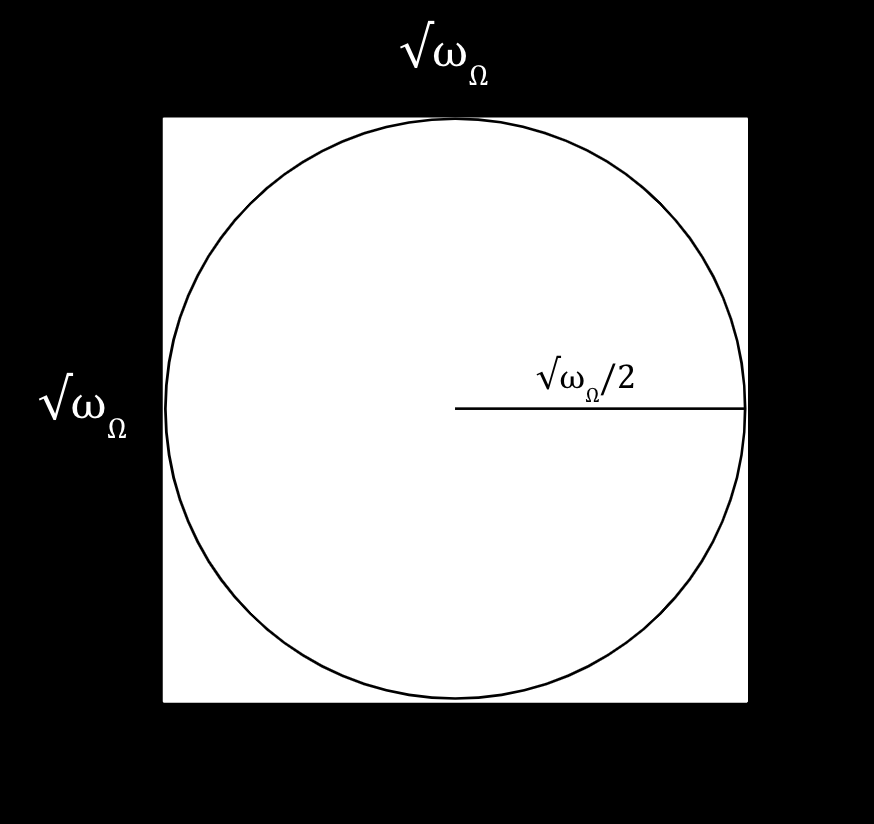
\includegraphics[width=1\linewidth]{Screenshot 2026-03-11 at 05.54.01.png}
    \caption{The largest physically meaningful circle in $\mathbb{R}_\Omega^2$, 
    inscribed within the largest possible finite square of side length 
    $\sqrt{\omega_\Omega}$ and area $\omega_\Omega$. The circle has radius $\frac{\sqrt{\omega_\Omega}}{2}$
    and circumference $\pi\sqrt{\omega_\Omega}$.}
    \label{fig:hyperfinite-circle}
\end{figure}

The side count remains $\sqrt{\omega_\Omega}$ and side length increases to $\pi$. The side count is fixed, as polygons are traditionally ``static'' structures, which will not spontaneously change their physical geometry when scaled (unless below atomic thresholds). The apothem at this new radius is:
\begin{align*}
a &= \frac{\sqrt{\omega_\Omega}}{2}\cos\left(\frac{\pi}{\sqrt{\omega_\Omega}}\right) \\[0.5em]
&= \frac{\sqrt{\omega_\Omega}}{2}\left(1 - \frac{\pi^2}{2\omega_\Omega} + \cdots\right) \\[0.5em]
&= \frac{\sqrt{\omega_\Omega}}{2} - \frac{\pi^2}{4}\sqrt{\varepsilon_\Omega} + \cdots
\end{align*}

The apothem-circumradius difference is therefore:
$$r - a = \frac{\pi^2}{4}\sqrt{\varepsilon_\Omega} \approx 2.47\sqrt{\varepsilon_\Omega}$$Since $2.47\sqrt{\varepsilon_\Omega} > \sqrt{\varepsilon_\Omega}$, this 
difference is \textbf{no longer zero-equivalent}. The polygon has lost 
equidistance - it no longer satisfies even the one condition it could 
previously meet. To restore circularity, the side count would need to increase 
while edge length remains $\sqrt{\varepsilon_\Omega}$. But polygons do not 
dynamically add sides - they are static structures.\\\\
This is the definitive physical failure. A polygon that satisfies circularity 
at one scale will fail at another, because \textit{radial length is a factor in the equation}. Therefore, \textbf{physical circles cannot maintain 
circularity under scaling.} And this leads directly to the conclusion of this 
section.

\subsubsection{The Need for a Virtual Definition}

All three physical limitations - local flatness, the impossibility of 
smoothness, and scale-dependent failure - point to the same conclusion. A 
circle cannot be defined purely physically in $\mathbb{R}_\Omega^2$. Any 
physical polygon, no matter how carefully constructed, is at best a momentary 
approximation that degrades under transformation.\\\\
The solution is to define a circle \textit{virtually} - through geometric data. This geometric data would then  instruct the physical figure on how to behave, allowing it to dynamically 
restructure as it scales. This is where the virtual definition of a circle, 
and with it, division by zero, finally enters the framework.

\subsection{Virtual Definition of a Circle}

As the preceding analysis has shown, a physically perfect circle is 
unachievable in $\mathbb{R}_\Omega^2$. We can construct a polygon that 
satisfies equidistance, minimizes edge length to $\sqrt{\varepsilon_\Omega}$, 
and maximizes side count - but none of this prevents the figure from losing 
circularity under scaling. Maintaining circularity at every scale would require 
the figure to \textit{dynamically restructure itself} - adding sides, adjusting 
geometry - as it grows or shrinks. Physical polygons cannot do this. They are 
static structures.\\\\
Dynamic geometry is, however, achievable - through \textbf{geometric data}. 
Rather than defining a circle as a physical figure alone, we define it as a 
physical figure carrying virtual geometric data that encodes how it should 
behave. This data acts as an instruction: when the circle scales, the virtual 
definition tells the physical structure to increase its side count while 
maintaining atomic edge length. The physical figure follows this instruction, 
maintaining circularity at every scale.\\\\
A circle in $\mathbb{R}_\Omega$ is therefore not a plain geometric figure. 
\textbf{It is a virtual one} - a physical structure with a virtual definition 
encoded inside it. Once we establish what that virtual definition is, all that 
remains is to encode it into the physical figure, allowing it to react and 
restructure dynamically. That is how circles - and curvature as a whole - are 
defined in this number system.

\subsubsection{Maintenance of Atomic Side Length}

This first aspect of defining a circle is utilizing an idea which was briefly introduced in the previous chapter. Recall from Chapter 7 the concept of geometric encoding: a physical structure can carry virtual geometry different from its physical geometry  governing its behavior. Specifically, we demonstrated that a line of physical length $\sqrt{\varepsilon_\Omega}$ could carry the virtual geometry of a zero-dimensional point, making it resistant to scaling, making it so multiplying by any factor $k$ leaves the physical length unchanged. What we do now is finally apply this concept to \textbf{circles}, by encoding this behavior onto physical circles (regular polygons of $\frac{P}{\sqrt{\varepsilon_\Omega}}$).\\\\Consider a line segment of physical length $\sqrt{\varepsilon_\Omega}$ encoded with virtual geometry: a zero-dimensional point.

\begin{figure}[H]
    \centering
    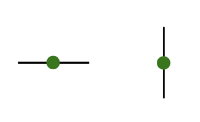
\includegraphics[width=0.3\linewidth]{Screenshot 2026-03-19 at 07.29.17.png}
    \caption{Line segments of length $\sqrt{\varepsilon_\Omega}$, (differing orientations) with virtual zero-dimensional geometry.}
\end{figure}

\begin{table}[H]
\centering
\begin{tabular}{|l|c|}
\hline
\textbf{Representation} & \textbf{Edge Length} \\
\hline
Physical & $\sqrt{\varepsilon_\Omega}$ \\
Virtual & $0$ \\
\hline
\end{tabular}
\caption{Physical and virtual edge length of an atomically encoded segment.}
\label{tab:edge-encoding}
\end{table}If we arrange enough of these segments properly to form a regular polygon of a particular radial length,  satisfying the condition of physical circularity (points are equidistant) we begin to have something that not only appears to be a circle, but also behaves a bit how we want it to - as its edge lengths don't increase when scaled.

\begin{figure} [H]
    \centering
    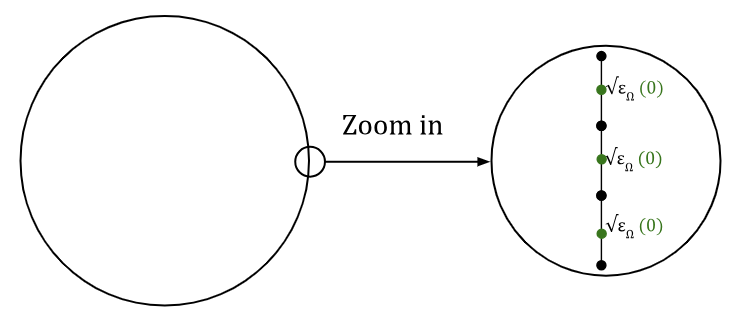
\includegraphics[width=1\linewidth]{Screenshot 2026-02-14 at 11.09.57.png}
    \caption{Taking and arranging the side lengths of actual length $\sqrt{\varepsilon_\Omega}$ and of virtual geometry 0 to form a physical ``circle''}
    \label{fig:placeholder}
\end{figure}

Moreover, since each edge has the minimal length $\sqrt{\varepsilon_\Omega}$, we also have this figure be ``as smooth as possible''. At a specific circumperimeter $P$ (the physical perimeter), the polygon has:
$$\text{Physical side count} = \frac{P}{\sqrt{\varepsilon_\Omega}}$$\\\\This structure satisfies circularity conditions.

\subsubsection{The Problem} 
These segments resist scaling. Just as a line encoded with point-geometry remains fixed under multiplication, a polygon built from such segments cannot grow or shrink. Scaling the figure by a factor of 2 leaves the edge lengths unchanged: the polygon does not expand. A true circle must scale, therefore this definition alone does not suffice.

\begin{figure} [H]
    \centering
    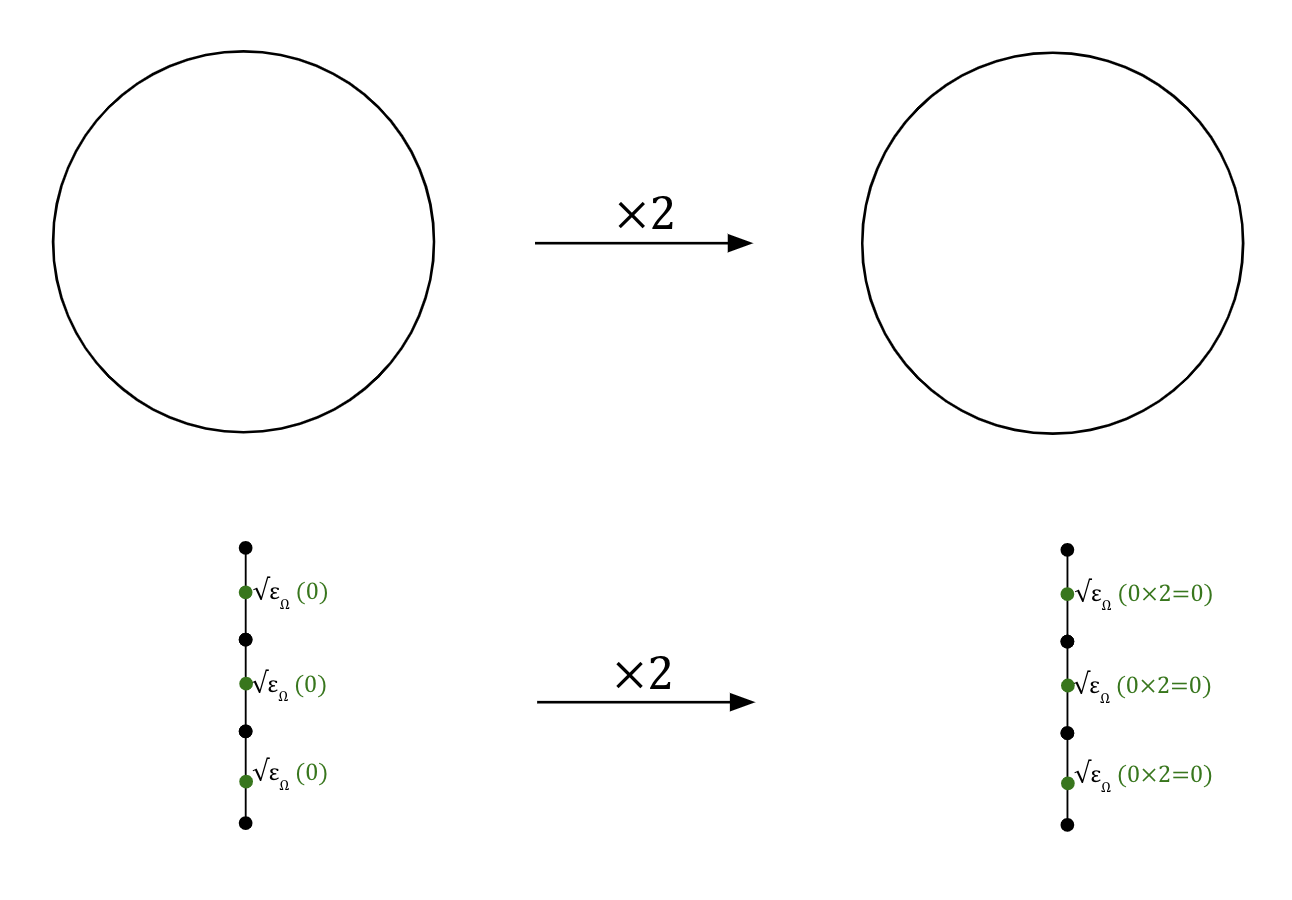
\includegraphics[width=1\linewidth]{Screenshot 2026-02-14 at 11.45.42.png}
    \caption{Inert physical geometry as a consquence of virtual geometry}
    \label{fig:placeholder}
\end{figure}So we face a question: how can we construct a figure that maintains atomic edge length ($\sqrt{\varepsilon_\Omega}$) while allowing circumference to increase?\\The answer isn't that this approach is wrong, it is just \textit{incomplete}. The solution to the problem is to actually add to it, which is achieved by defining the virtual structure of the circle to not just be some arbitrary set of virtual points arranged in space to form a circular pattern, but rather to be part of a larger \textit{virtual} structure - this will allow to give the physical a dynamic geometry, while maintaining a minimum edge length. And the way this is achieved, is actually by division by zero.

\subsubsection{The Definition of Circularity Through Division by Zero}

We have established that no physical polygon can maintain circularity under 
scaling - and that the only resolution is a virtual one. Through geometric 
encoding, a circle is defined in two parts: a physical structure, and a virtual 
structure integrated inside it. The physical structure manifests the circle in 
space; the virtual structure instructs it how to behave under transformation. 
And as we shall now see, that virtual structure is defined through division 
by zero.

A circle is virtually defined as a regular polygon with:
\begin{itemize}
\item \textbf{Virtual side length:} $0$ (traditional zero, not sub-infinitesimal)
\item \textbf{Virtual side count:} $\frac{C}{0}$ (circumference divided by zero)
\end{itemize}

This is not a metaphor. It is the literal virtual geometric definition of a 
circle - and although it sounds absurd, it is in truth the entire argument of 
this paper condensed into a single idea. In every number system prior to this 
one, a circle could only ever be defined as a regular polygon whose side 
lengths are \textit{approaching} zero and whose side count is 
\textit{approaching} infinity - every polygon in the sequence, more sides, 
shorter edges, closer apothem, converging toward something it could never 
reach. Here, we let the side length \textbf{be} zero and the side count 
\textbf{be} infinity - not as an approximation, not as a limit, but as a 
\textit{virtual definition}. In $\mathbb{R}_\Omega$, we do not merely approach this 
definition. We \textit{reach} it.\\\\
To verify this, recall the apothem formula:
$$a = r\cos\left(\frac{\pi}{n}\right)$$

In the reals, the limit as $n \to \infty$ gives:
$$\lim_{n \to \infty} r\cos\left(\frac{\pi}{n}\right) = r$$

The apothem approaches the circumradius but never reaches it. In 
$\mathbb{R}_\Omega^2$, we let $n$ \textit{be} $\frac{C}{0}$ - not approaching 
infinity, but actually being it:
$$r\cos\left(\frac{\pi}{\frac{C}{0}}\right) = r\cos\left(\frac{\pi \times 0}{C}\right) = r\cos(0) = r \times 1 = r$$

The apothem \textbf{exactly equals} the circumradius - not approximately, not 
to within zero-equivalent precision, but exactly. The virtual circle satisfies 
equidistance perfectly, because its side count is not merely hyperfinite but 
genuinely infinite.\\\\
The side length follows directly from the standard perimeter formula:
$$P = n \times s$$

Substituting $n = \frac{C}{0}$ and $P = C$:
$$C = \frac{C}{0} \times s$$

Solving for $s$:
$$s = \frac{C}{\frac{C}{0}} = \frac{C \times 0}{C} = 0$$

The virtual side length is exactly $0$ - traditional zero. This is consistent 
with the definition:
$$C = \frac{C}{0} \times 0 \quad \checkmark$$ \textbf{Note:} The algebra behind this claim - specifically, why 
$\frac{C}{0} \times 0 = C$ holds consistently rather than collapsing to 
zero - will be established in the following subsection on algebraic 
consistency. For now, division by zero is treated conceptually.

\subsubsection*{Why This Definition Works:}

Circles are traditionally considered as being completely “circular” and purely “smooth” - with no edges or sides. Although this is a ``naive'' way of thinking about it, a regular polygon of side length zero \textit{does} naively fit this description. \\The second, and more \textit{legitimate} argument is that this definition gives physical circles the instruction they need in order to \textit{maintain} circularity. If we set the  virtual side length to $0$, then scaling annihilates the edge lengths, making it so that multiplying by any factor $k$ leaves individual edges unchanged:
$$s_{\text{new}} = 0 \times k = 0$$However, this definition \textit{does} allow the circumference to change. For example, scaling by $k$ would make it so the circumference would essentially just ``change'' the side count (technically \textit{side arrangement}, as will be seen in the next section), leaving a new figure with a different side count:
$$C \to kC \quad \Rightarrow \quad \frac{C}{0} \to \frac{kC}{0}$$This creates dynamic geometry: the circumference can increase (more ``sides'' are generated) while each individual side remains virtually zero-length.

\begin{figure} [H]
    \centering
    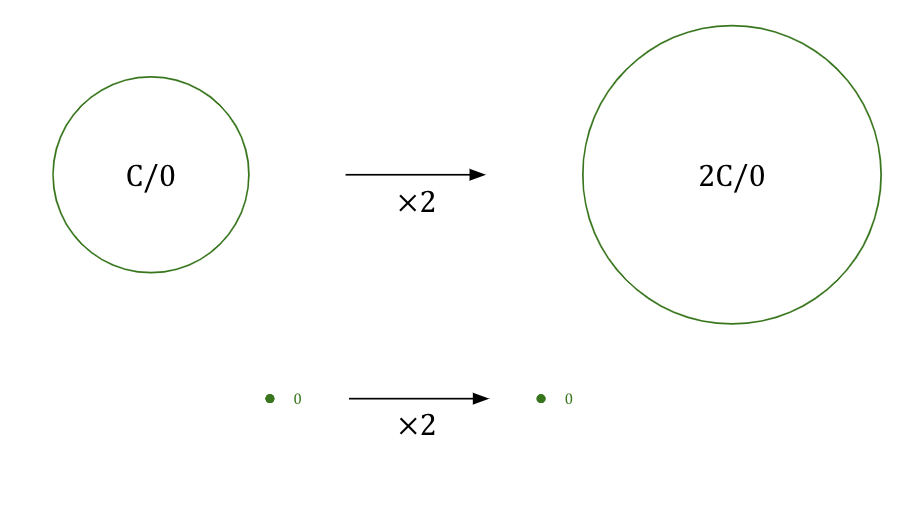
\includegraphics[width=1\linewidth]{Screenshot 2026-02-14 at 12.09.42.png}
    \caption{Visualization of the virtual definition of a circle, in which scaling will increase circumference, however individual ``side lengths'' remain the same}
    \label{fig:placeholder}
\end{figure}

Physically, these virtual zero-length sides manifest as atomic segments of length $\sqrt{\varepsilon_\Omega}$: the geometric encoding we discussed. Increasing the circumference generates more physical segments, but each maintains the atomic threshold length.

\subsubsection{Full Definition of a Circle in $\mathbb{R}_\Omega^2$}

In $\mathbb{R}_\Omega^2$, a circle exists as two entities simultaneously.\\\\
\textbf{Virtual geometry (the definition):}
\begin{itemize}
\item Side length: $0$
\item Side count: $\frac{C}{0}$
\item Circumference: $C$
\end{itemize}

\textbf{Physical geometry (the manifestation):}
\begin{itemize}
\item Side length: $\sqrt{\varepsilon_\Omega}$
\item Side count: $\frac{P}{\sqrt{\varepsilon_\Omega}}$ (where $P$ is the 
physical perimeter, hereafter called the \textit{circumperimeter})
\end{itemize}

\begin{table}[H]
\centering
\begin{tabular}{|l|c|c|}
\hline
\textbf{Property} & \textbf{Physical} & \textbf{Virtual} \\
\hline
Side length & $\sqrt{\varepsilon_\Omega}$ & $0$ \\
Side count & $\frac{P}{\sqrt{\varepsilon_\Omega}} = P\sqrt{\omega_\Omega}$ & $\frac{C}{0}$ \\
Apothem $= r$? & Zero-equivalent (sub-infinitesimal) & Zero (traditional zero) \\
Smooth? & Approximately, but not atomically (staircase) & Completely (side length is zero) \\
\hline
\end{tabular}
\caption{Physical vs. virtual properties of a circle in $\mathbb{R}_\Omega^2$.}
\label{tab:physical-virtual-circle}
\end{table}A circle is fully defined as being a physical regular polygon with virtual geometric data integrated inside of
it, which dictates how it behaves under scaling. This virtual data is precisely what 
distinguishes a circle from a regular polygon - even when the two are 
physically identical.\\\\
To see why, consider a circle of circumperimeter 1. It physically possesses 
a side count of $\frac{1}{\sqrt{\varepsilon_\Omega}} = \sqrt{\omega_\Omega}$ 
and edge length $\sqrt{\varepsilon_\Omega}$. Now consider an exact physical 
replica: a $\sqrt{\omega_\Omega}$-gon of the same perimeter. At this scale, 
the two figures are indistinguishable. Virtually, however, they are not. The 
circle carries the virtual definition as its geometric data. The polygon does 
not.\\\\
This difference only becomes apparent under scaling. When stretched by a 
factor of 2, the circle increases its side count while maintaining edge length 
$\sqrt{\varepsilon_\Omega}$ - its virtual definition instructs it to behave as 
a polygon of side length zero, so scaling generates more sides rather than 
longer ones. The polygon, carrying no such instruction, simply scales its edge 
length upward while its side count remains fixed.

\begin{figure}[H]
    \centering
    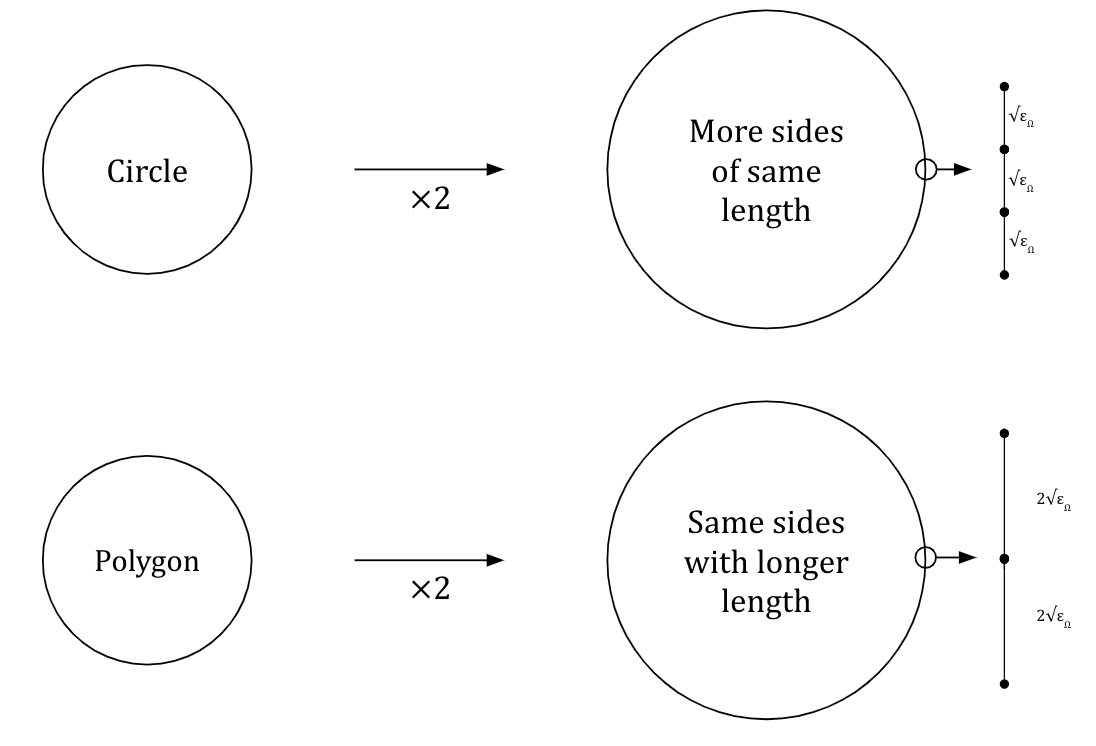
\includegraphics[width=1\linewidth]{Screenshot 2026-02-14 at 14.18.21.png}
    \caption{Scaling behaviour of a circle vs. a regular polygon in 
    $\mathbb{R}_\Omega^2$. The circle increases side count while maintaining 
    atomic edge length; the polygon maintains side count while edge length 
    grows.}
    \label{fig:circle-vs-polygon-scaling}
\end{figure}

\begin{table}[H]
\centering
\begin{tabular}{|l|c|c|}
\hline
\textbf{Property} & \textbf{Scale factor 1} & \textbf{Scale factor 2} \\
\hline
\hline
\multicolumn{3}{|c|}{\textbf{Circle}} \\
\hline
Circumperimeter & 1 & 2 \\
Side count & $\sqrt{\omega_\Omega}$ & $2\sqrt{\omega_\Omega}$ \\
Side length & $\sqrt{\varepsilon_\Omega}$ & $\sqrt{\varepsilon_\Omega}$ \\
Virtual side geometry & \multicolumn{2}{c|}{Zero-dimensional ($s = 0$)} \\
\hline
\hline
\multicolumn{3}{|c|}{\textbf{Regular polygon ($\sqrt{\omega_\Omega}$-gon)}} \\
\hline
Perimeter & 1 & 2 \\
Side count & $\sqrt{\omega_\Omega}$ & $\sqrt{\omega_\Omega}$ \\
Side length & $\sqrt{\varepsilon_\Omega}$ & $2\sqrt{\varepsilon_\Omega}$ \\
Virtual side geometry & \multicolumn{2}{c|}{Line segment (same as physical)} \\
\hline
\end{tabular}
\caption{Scaling behaviour: circles adjust side count, polygons adjust side 
length.}
\label{tab:circle-vs-polygon-scaling}
\end{table}

From this point forward, the word ``circle'' refers specifically to a regular 
polygon \textbf{with} this virtual geometric data. A ``regular polygon'' means 
a figure \textbf{without} it. Physically identical, virtually distinct.\\\\
The virtual definition is what the physical has always been approximating. 

\section{Chapter 9 - Division by zero}

In this number system, division by zero was defined by actuality as being \textit{infinity}, establishing the connection of zero-equivalent sub-infinitesimal data to that of infinite-equivalent specific infinite data, virtually defining one as being the reciprocal of the other. For every ``zero-equivalent'' sub-infinitesimal data, there is an ``infinite-equivalent'' reciprocal with specific infinite data. The nature of $\infty$ being a value ``beyond actuality'' and not in $\mathbb{R}_\Omega$ gives it a reciprocal relationship to zero, and also an unsigned nature.\\\\Up until this chapter, division by the traditional zero - the zero with the 
multiplicative annihilator property - was left undefined in this framework. 
We have now defined it as the ``side count'' of the virtual structure of a circle, governing circularity.
Specifically, a circle is virtually defined as a regular polygon of side length 
zero and side count $\frac{C}{0}$ - enabling curvature, in which scaling 
upwards or downwards maintains atomic edge length while increasing physical 
side count accordingly. This virtual definition is not a distinct geometric 
figure existing somewhere in space. It is better understood as an 
\textbf{algorithm}: a set of instructions encoded into the physical figure, 
governing how it constructs and maintains circularity at any scale.\\\\However, what does all of this mean specifically? How can we further make sense of this definition? We've \textbf{applied} division by zero and claimed it to be ``a set of instructions'' that circles follow in this number system, however, this doesn't really fully define nor solve division by zero completely - it is an ``application'' of the concept, but not really a definition of it. \\\\Which is why in this section, we shall elaborate upon and further flesh out this definition of division by zero, turning this conceptual definition into a definitive one.

\subsubsection{\U{} Notation}

To formalize division by zero, we introduce a special notation: \textbf{\U{}} (katakana ``U'', pronounced like the English letter).\\\U{} notation denotes the \textbf{virtual} result of division by zero using a \textbf{traditional zero} - not a sub-infinitesimal data expression. This distinction is necessary because in $\mathbb{R}_\Omega \cup \infty$, division by zero always produces infinity by actuality, regardless of whether the zero is traditional or sub-infinitesimal. This means that \textbf{by actuality, all divisions by zero are infinite:}
$$\frac{1}{0} = \infty$$

This holds whether the zero is sub-infinitesimal:
\begin{align*}
0 &\to_v 0_{[0.5\varepsilon_\Omega]} \\
\frac{1}{0} &=_v \infty_{[2\omega_\Omega]}
\end{align*}

or traditional:
\begin{align*}
0 &\to_v 0_{[0]} \\
\frac{1}{0} &=_v \text{\U}_1
\end{align*}

Both have the same actual value:
$$\infty_{[2\omega_\Omega]} \  _a{=}_a \  \text{\U}_1 \quad \text{(both are infinite)}$$But they differ \textbf{virtually}, with their geometric data and algebraic behavior being completely different:
$$\infty_{[2\omega_\Omega]} \  _v{\neq}_v \  \text{\U}_1$$

\textbf{General form:}

For any $n \neq 0$:
$$0\to_v0_{[0]}$$
$$\frac{n}{0} = \infty =_v \text{\U}_n$$
\textbf{Examples:}
$$0\to_v0_{[0]}$$
$$\frac{1}{0} = \infty, \quad \frac{1}{0} =_v \text{\U}_1$$
$$\frac{2}{0} = \infty, \quad \frac{2}{0} =_v \text{\U}_2$$
$$\frac{\pi}{0} = \infty, \quad \frac{\pi}{0} =_v \text{\U}_\pi$$

\subsubsection{Understanding \U}

\U - is understood as being a \textbf{specific infinite data} of infinity - although it is a wholly different classification of specific infinite data than specific infinite data larger than $\omega_\Omega$. 
\\\U$_C$ is understood as being on the surface, the (virtual) solution to division by zero, in which zero is a ``traditional'' zero. $$\frac{1}{0}=\text{\U}_1$$However, conceptually, and as previously established, \U{} isn't just some number or value - it is representative of the ``virtual'' side count of a virtual circle. It isn't a computable or ``meaningful'' value, as it isn't defined as being some specific actual value - by actuality we established that it was just infinite. By virtuality, we've defined it as being a specific infinite data of infinity acting as an \textbf{instruction code} specifying not only ``how'' to sum up zeroes, but how to \textit{arrange} these zeroes to form circularity and curvature in 2-D space in $\mathbb{R}_\Omega^2$.

\subsubsection{Conceptually Understanding Division by Zero Through Zero-Triangles}

To understand what \U$_C$ is on a simple conceptual level, we define a virtual circle as being cut up by infinitely many ``zero arc edge length triangles'' (or simply zero-triangles). \\In traditional calculus, a circle can be approximated by decomposing it into 
infinitesimally thin wedges - like cutting a pizza into an infinite number of 
slices. Each wedge is approximately a triangle with two radial edges of length 
$r$ and one arc edge of length $\frac{C}{n}$, where $n$ is the number of 
wedges. The virtual circle takes this idea to its logical conclusion: each 
wedge has two radial edges of length $r$ and one arc edge of length exactly 
$0$.

\begin{figure}[H]
    \centering
    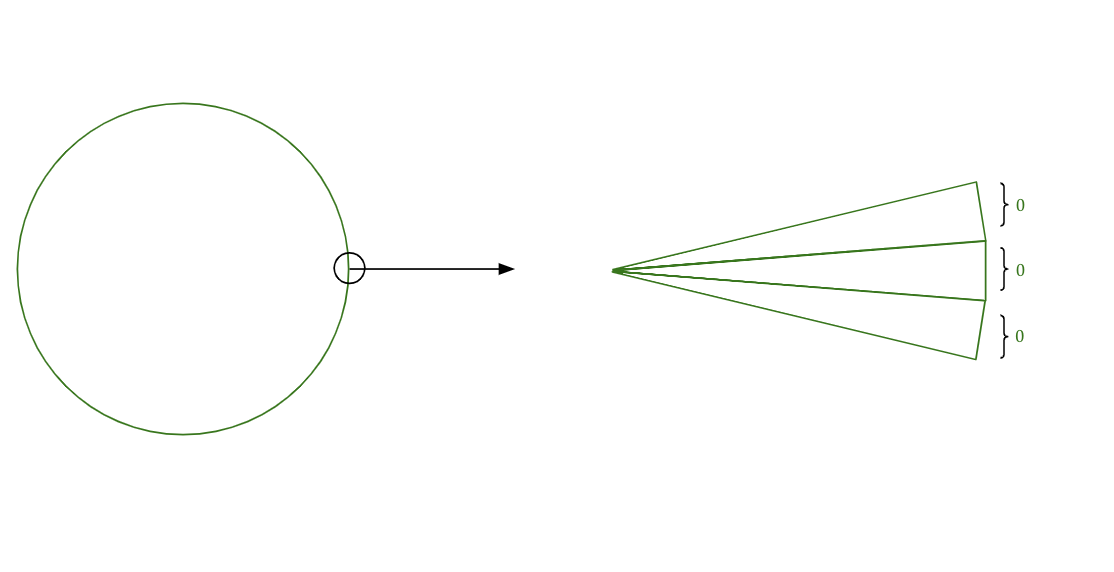
\includegraphics[width=1\linewidth]{Screenshot 2026-03-08 at 14.50.43.png}
    \caption{A virtual circle decomposed into zero-triangles. Each wedge has two 
    radial edges of length $r$ and one arc edge of virtual length 
    $0$ (green).}
    \label{fig:zero-triangles}
\end{figure}The virtual circle is a collection of these zero-triangles arranged radially 
around the center. Each triangle contributes an arc of length $0$, yet the 
total circumference is:
$$C = \frac{C}{0} \times 0$$But this is not a traditional sum. Adding these zeroes (which in this case represent the \textit{zero-triangles}) ``simply'' does not produce a nonzero 
value:
$$0 + 0 + 0 + \cdots \neq C$$ Because of the fact that $0\times n=0$. However, this is where \U$_C$ differs from simply being a traditional summation, and does its work. Unlike a regular ``number'', \U$_C$ does not merely sum up the 
zero-triangles - it also \textit{arranges} them. \U$_C$ encodes a geometric 
instruction: a specification of how the zero-triangles are to be positioned 
in space so that their arrangement produces a circle of circumference $C$.

\begin{figure}[H]
    \centering
    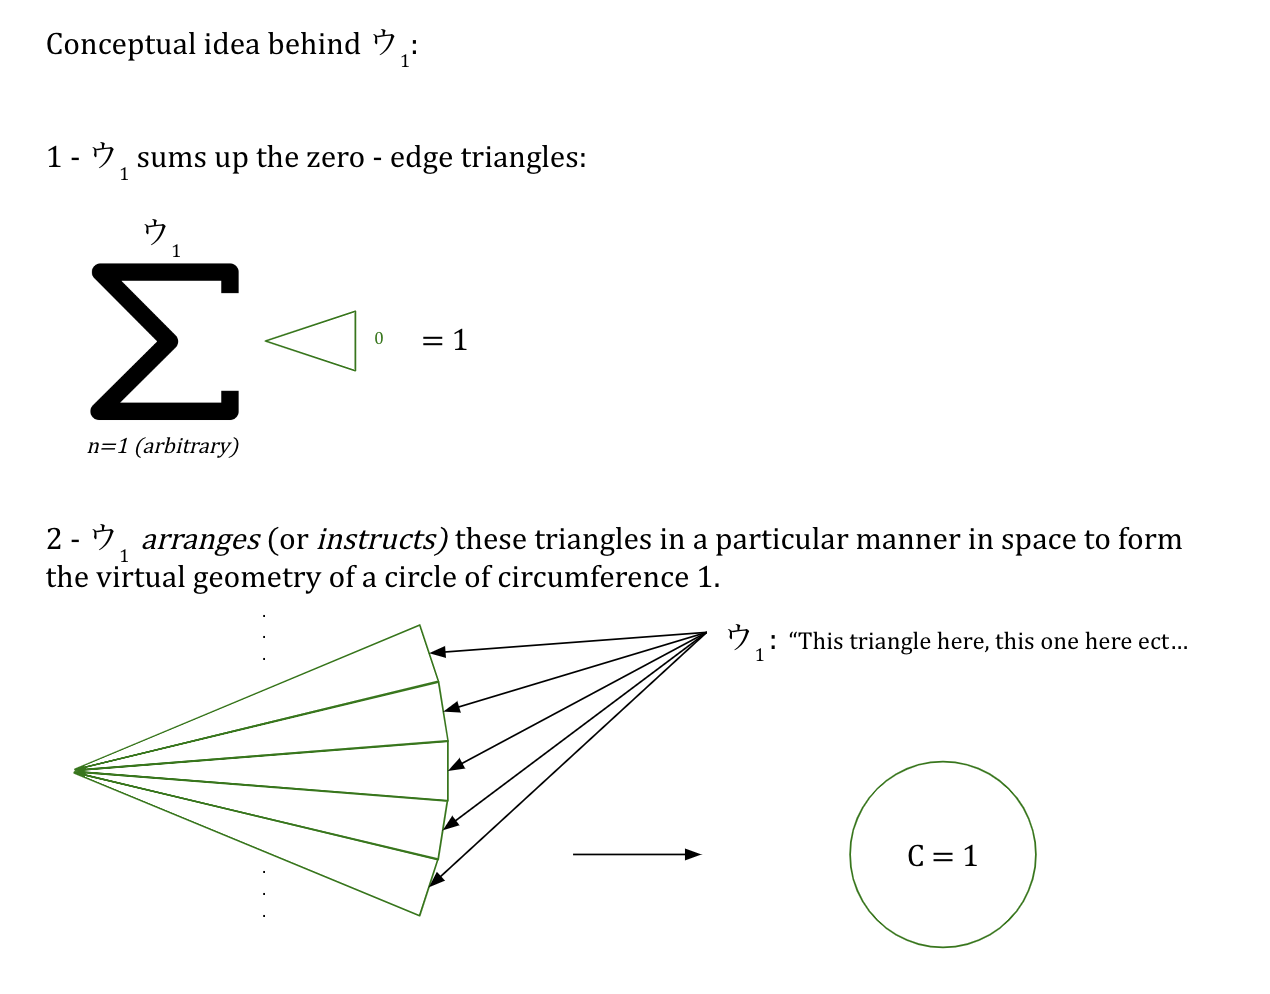
\includegraphics[width=1\linewidth]{Screenshot 2026-03-08 at 14.50.58.png}
    \caption{The conceptual role of \U$_1$. First, \U$_1$ sums the 
    zero-edge triangles. Then, it \textit{arranges} them in space - 
    instructing each triangle to occupy a specific radial position - 
    producing a virtual circle of circumference 1.}
    \label{fig:u1-concept}
\end{figure}

When we write:
$$\frac{C}{0} \times 0 = C$$We are saying: take a zero-edge triangle and sum infinitely many of them, but 
\textbf{arrange} them radially according to the instructions encoded in 
\U$_C$, producing a circle of circumference $C$.\\\\
Different circumferences require different arrangement codes entirely:

\begin{figure}[H]
    \centering
    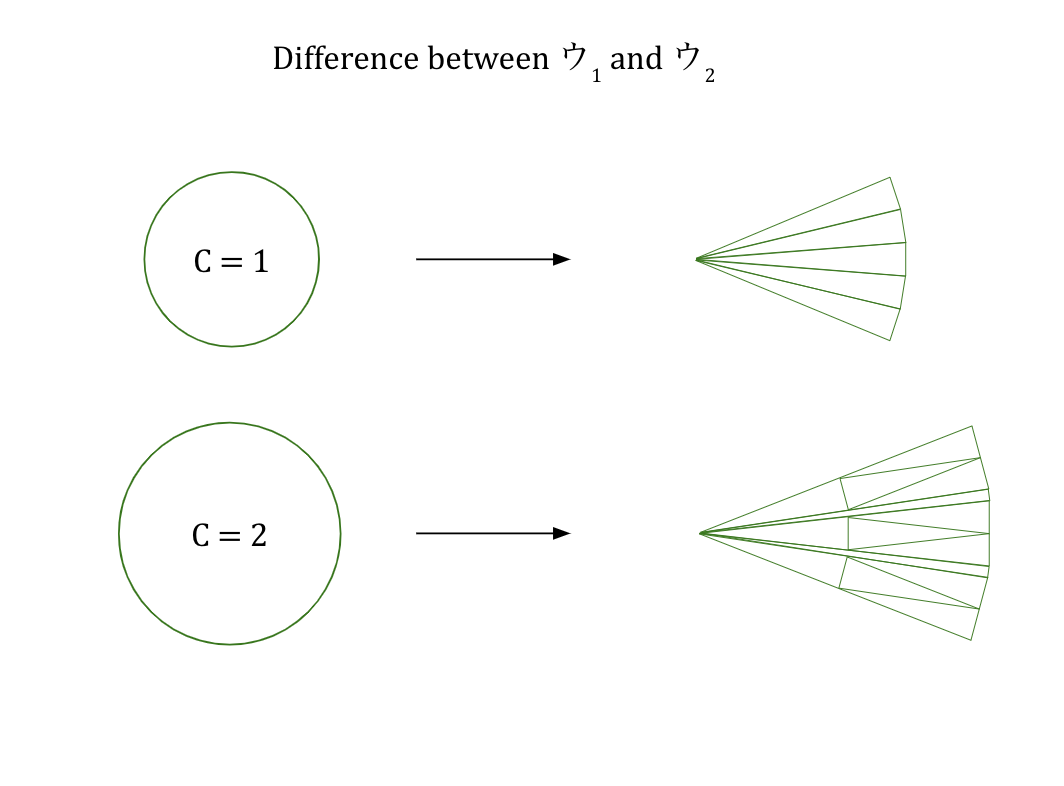
\includegraphics[width=0.6\linewidth]{Screenshot 2026-03-08 at 15.10.34.png}
    \caption{The difference between \U$_1$ and \U$_2$. Both consist of 
    infinitely many zero-triangles, but the arrangement codes are entirely 
    distinct - \U$_1$ produces a circle of circumference 1, \U$_2$ a circle 
    of circumference 2. The difference is not in quantity but in spatial 
    structure.}
    \label{fig:u1-u2-difference}
\end{figure}

\begin{itemize}
\item \U$_1$: sums and arranges $\frac{1}{0}$ zero-triangles into a circle of 
circumference 1
\item \U$_2$: sums and arranges $\frac{2}{0}$ zero-triangles into a circle of 
circumference 2
\item \U$_{2\pi}$: sums and arranges $\frac{2\pi}{0}$ zero-triangles into a unit 
circle
\end{itemize}

The distinction between these is not in how many triangles are involved - 
``how many'' loses meaning at this scale. The distinction is entirely in 
\textbf{how they are arranged in space}. This is why \U$_1 \ _v{\neq}{}_v$ \U$_2$ 
despite both being infinite: they are different geometric instructions, 
encoding different spatial structures. And this is why division by zero in 
this framework is not simply infinity - it is a \textbf{geometrically encoded 
infinity}. Its actual value is infinity, but its virtual data encodes the 
specific spatial arrangement that defines a circle of circumference $C$.

\subsubsection{Important Note: The True Nature of \U$_C$}

The zero-triangle construction above is a useful conceptual tool, but it is 
important to clarify what \U$_C$ actually \textit{is} - because the virtual 
polygon of side length zero is an idealization, not a literal entity. There 
is no regular polygon of side count $\frac{C}{0}$ and side length $0$ existing 
somewhere in some exotic geometric space. No such figure physically or even 
\textit{virtually} exists as a structure in $\mathbb{R}_\Omega^2$.\\\\
What \U$_C$ actually is, is far simpler and more abstract: it is 
\textbf{metadata}. Recall from Chapter 1 the concept of mathematical data - 
the idea that numbers can carry qualitative information beyond their actual 
value, in the same way that zero apples and zero bananas share the same actual 
value of zero while carrying different virtual information. \U$_C$ is precisely 
this concept applied to infinity. It is an infinity carrying specific metadata: 
the instruction of how to sum and arrange zeroes so that their arrangement 
produces curvature of circumference $C$.\\\\
In this sense, \U$_C$ is less like a geometric figure and more like an 
algorithm - a set of instructions that infinity can possess, which when applied 
to a physical structure, governs how that structure constructs and maintains 
circularity. The virtual polygon of side length zero is simply the most 
intuitive way to \textit{visualize} these instructions. The instructions 
themselves are just metadata.

\begin{figure}[H]
    \centering
    \begin{subfigure}[t]{0.45\textwidth}
        \centering
        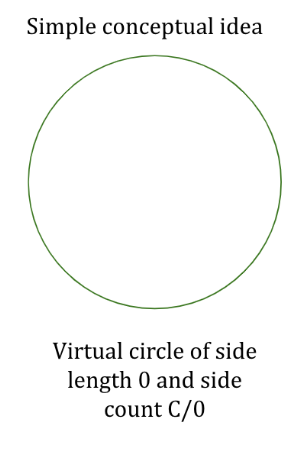
\includegraphics[width=\linewidth]{Screenshot 2026-03-20 at 00.31.24.png}
        \caption{Simple conceptual idea: a virtual circle of side length $0$ and side count $\frac{C}{0}$}
    \end{subfigure}
    \hfill
    \begin{subfigure}[t]{1\textwidth}
        \centering
        \begin{lstlisting}[language=Python]
# U_C : curvature instruction code
# Input  : circumference C

def U(C):

    # Step 1: define zero as a zero-triangle
    zero = ZeroTriangle(arc = 0, r = C/(2*pi))

    # Step 2: create C/0 copies of zero
    triangles = repeat(zero, count = C/0)

    # Step 3: arrange them radially
    arrange_in_circle(triangles, origin = (0,0))

    # Step 4: return the circle
    return Circle(circumference = C)

# Actual value:  infinity
# Virtuality: U_C
        \end{lstlisting}
        \caption{More accurate yet abstract idea: \U$_C$ as pure metadata, a code instructing how zeroes are summed and arranged to produce curvature of circumference $C$}
    \end{subfigure}
    \caption{Two interpretations of \U$_C$}
    \label{fig:u-interpretations}
\end{figure}

This distinction matters because it clarifies what division by zero 
\textit{is} in this framework - not a bizarre infinite polygon, but a specific 
class of metadata that infinity can carry, encoding geometric structure. Just 
as the absence of a banana carries the virtual essence of ``banana'' without 
any banana being present, \U$_C$ carries the virtual essence of a circle of 
circumference $C$ without any such circle existing as a literal figure.

\subsubsection{Curvature as Geometric Data}

The virtual definition of circles extends naturally beyond closed curves. 
Division by zero is not merely the virtual side count of a circle - it is the 
fundamental geometric data that encodes \textbf{curvature itself} at any point 
on any curve.\\\\
In Euclidean geometry, curvature at a point on a curve is defined by the 
\textbf{osculating circle} - the unique circle that best approximates the curve 
locally at that point. The radius of this circle, $\rho$, is the 
\textbf{radius of curvature}: the smaller $\rho$ is, the sharper the curve 
at that point.

\begin{figure}[H]
    \centering
    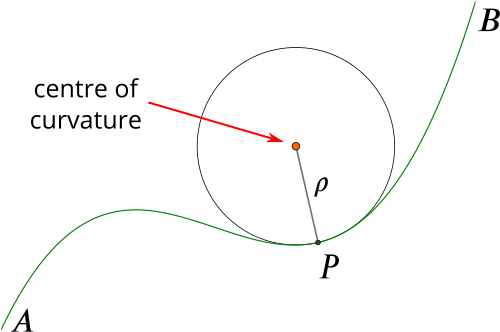
\includegraphics[width=0.5\linewidth]{centre-of-curvature.png}
    \caption{A curve with its osculating circle at a point $P$. The radius 
    $\rho$ extends from $P$ to the centre of curvature. Image 
    source: \cite{t}}
    \label{fig:curvature-radius}
\end{figure}

In $\mathbb{R}_\Omega^2$, every curve - whether closed (circles, ellipses) or 
open (parabolas, arbitrary curves) - is physically approximated by discrete 
atomic edge segments of length $\sqrt{\varepsilon_\Omega}$. Each segment is 
physically straight and cannot curve. But each segment is not merely a line - 
it carries virtual data. Specifically, each atomic edge carries the \U{} data 
corresponding to its local osculating circle: an edge at a point with radius 
of curvature $\rho$ carries the virtual data \U$_{2\pi\rho}$. This is the 
geometric data of the circle of circumference $2\pi\rho$ - the osculating 
circle at that point.

\begin{figure}[H]
    \centering
    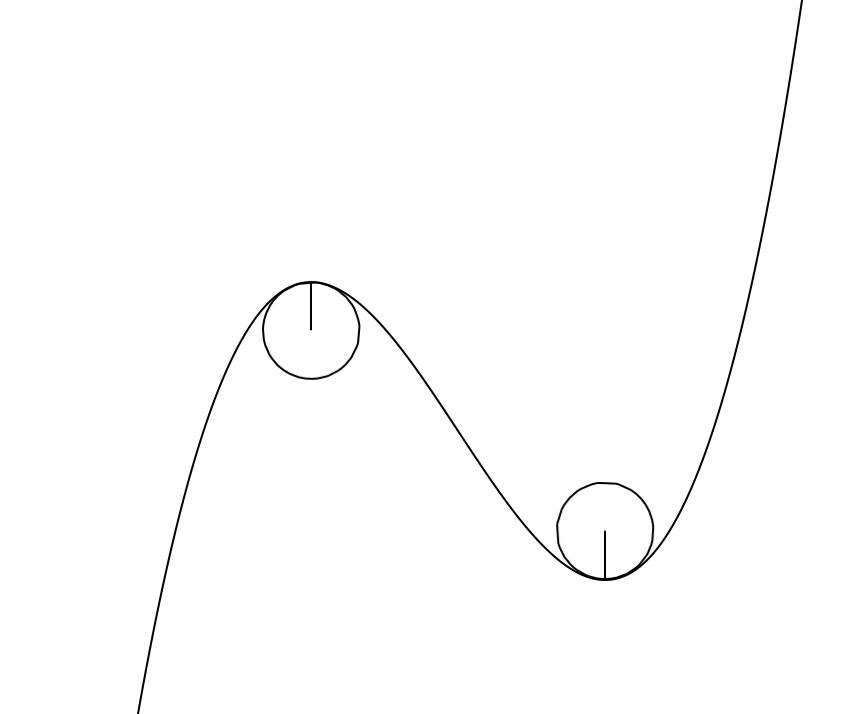
\includegraphics[width=0.6\linewidth]{Screenshot 2026-03-11 at 23.35.32.png}
    \caption{Two osculating circles on a curve at its local maximum and local 
    minimum. Although geometrically distinct points, both carry identical 
    virtual curvature data \U$_{2\pi\rho}$ - in this case with radii of 
    curvature $\rho \approx 1.170$ and circumferences $C = 2\pi\rho \approx 
    7.351$. The physical edges at these points are straight atomic segments 
    of length $\sqrt{\varepsilon_\Omega}$; the curvature exists purely as 
    virtual data.}
    \label{fig:osculating-circles}
\end{figure}

\begin{table}[H]
\centering
\begin{tabular}{|l|c|c|}
\hline
\textbf{Property} & \textbf{Local Maximum} & \textbf{Local Minimum} \\
\hline
Position $(x_0, y_0)$ & $(-0.892,\ 0.313)$ & $(6.226,\ -6.880)$ \\
Radius of curvature $\rho$ & $\dfrac{25}{2\sqrt{114}} \approx 1.170$ & 
$\dfrac{25}{2\sqrt{114}} \approx 1.170$ \\[0.8em]
Circumference $C = 2\pi\rho$ & $\approx 7.351$ & $\approx 7.351$ \\
Virtual curvature data & \U$_{7.351}$ & \U$_{7.351}$ \\
Centre of curvature & $(-0.892,\ -0.857)$ & $(6.226,\ -5.710)$ \\
\hline
\end{tabular}
\caption{Quantitative curvature data at the local maximum and minimum of 
$y = 5\left(\frac{x}{5}\right)^3 - 8\left(\frac{x}{5}\right)^2 - 
2\left(\frac{x}{3}\right)$. Both points carry identical virtual curvature 
data \U$_{7.351}$ despite occupying different positions on the curve.}
\label{tab:curvature-data}
\end{table}

Different points on a curve carry different \U{} data - a sharp bend encodes 
a small $\rho$ and therefore a small osculating circumference \U$_{2\pi\rho}$, 
while a gentle curve encodes a large $\rho$ and a correspondingly large 
circumference.\\\\
\textbf{Curvature under scaling:} When a curve is scaled by factor $k$, 
every osculating circle scales with it. A circle of radius $\rho$ becomes 
a circle of radius $k\rho$, and its circumference scales accordingly:
$$2\pi\rho \to 2\pi k\rho$$

This is identical to the circle scaling argument established earlier: just 
as scaling a circle of circumference $C$ by factor $k$ sends 
$\frac{C}{0} \to \frac{kC}{0}$, scaling a curve sends the virtual curvature 
data at each point from \U$_{2\pi\rho}$ to \U$_{2\pi k\rho}$:
$$\text{\U}_{2\pi\rho} \to \text{\U}_{2\pi k\rho}$$

The physical edge length remains $\sqrt{\varepsilon_\Omega}$ throughout - 
unchanged, as always. Only the virtual data updates. Curvature under scaling 
is therefore entirely a virtual phenomenon: the physical geometry stays 
discrete and atomic, while the encoded osculating circle adjusts to reflect 
the new scale.\\\\
In this sense, \textbf{curvature in $\mathbb{R}_\Omega^2$ is not a physical 
property - it is a virtual one}. Every smooth curve is, physically, just a 
collection of atomic straight edges. What makes it curved is the \U{} data 
each edge carries - the encoded memory of which osculating circle it belongs 
to.

\subsubsection{Negative Division by Zero}

In this theory, the concept of \U{} extends to \textit{negative} division by zero. 

$$\frac{-1}{0} =_a \infty, \quad \frac{-1}{0} =_v \text{\U}_{-1}$$

By actuality, negative division by zero, just like all divisions by zero, is simply infinity by actual value.
$$\frac{-1}{0} = \frac{1}{0}$$

Virtually, however, they differ:
$$\frac{-1}{0} \ _v{}{\neq}{}_v \ \frac{1}{0}$$

However, this virtual distinction raises the question. If we stick purely to the simple conceptual idea that \U$_C$ is simply a ``side count'', does that mean that \U$_{-C}$ is a \textit{negative} count? Is it supposed to represent a circle of \textit{negative} circumference? Well, truth be told, this is actually an instance where our simple conceptual idea of ``zero triangles'' forming a circle fails, because a negative circumference is \textbf{meaningless}, and a negative circle does not exist, as circumference is an unsigned geometric quantity. \\\\
This is precisely where the \textit{algorithm} interpretation of \U{} becomes 
not just useful, but necessary. If \U$_C$ were a literal virtual figure - a 
polygon of side length zero floating somewhere in geometric space - then 
\U$_{-1}$ would be a geometric absurdity, a figure with negative circumference 
that cannot exist even virtually. But \U$_C$ is not a figure. It is a 
\textbf{code} - a set of instructions that infinity carries, governing how 
zeroes are arranged to produce curvature. And a code can have a negative 
parameter without requiring a negative geometric object to exist.\\\\
Under this interpretation, \U$_{-1}$ is the instruction code for a circle of 
circumference 1 traversed in the \textbf{opposite orientation}. In mathematics, 
counterclockwise traversal is conventionally positive and clockwise negative. 
\U$_1$ encodes counterclockwise arrangement of zero-triangles; \U$_{-1}$ 
encodes the same arrangement traversed clockwise. The magnitude of the 
circumference is identical - only the orientation differs. Negative division by zero does not produce a 
geometrically impossible figure - it produces a geometrically valid one with 
reversed orientation, encoded as metadata rather than manifested as a literal 
structure.

\subsection{Algebraic Consistency and Trivial Data}

This is the final subsection of the final chapter of the entire theory. 
Although division by zero has been defined geometrically in the preceding 
chapters, and this definition is internally consistent within the confines of this theory, geometry alone does not address the algebraic objections that have 
historically made division by zero undefinable. Defining division 
by zero has historically been rejected not merely because it lacks meaning, 
but because attempting to manipulate it algebraically produces contradictions. 
This subsection addresses those objections directly.
\\\\The resolution comes from the final and most fundamental form of mathematical 
data, one which was always implicitly present in the framework but never 
formally introduced. This final form of data is what we call \textbf{trivial data}. Trivial data addresses and resolves the algebraic inconsistencies that 
arise when division by zero is manipulated outside its geometric context.

\subsubsection{Trivial Data}

Let us return all the way back to the foundations of this theory - to Chapter 
1, and the original introduction of mathematical data. Data was introduced 
as a qualitative framework: a way of storing information about numbers 
beyond their actual value. We developed this concept in three forms 
throughout the theory:

\begin{itemize}
\item \textbf{Sub-infinitesimal data} - describes what happens when 
actuality fails as a result of the lower bound: $\frac{1}{2}\varepsilon_\Omega =_a 0$, 
yet the two are virtually distinct.
\item \textbf{Specific infinite data} - describes what happens when 
actuality fails as a result of the upper bound: $2\omega_\Omega =_a \infty$, 
yet different infinite data is virtually distinguishable.
\item \textbf{Geometric data} - describes how physical structures can 
encode behavioural instructions, preserving information when actuality 
fails. Most importantly it is used to define circularity by defining curvature through 
division by zero.
\end{itemize}

All three of these forms of data were built upon a single foundational 
idea introduced in Chapter 1: that different absences, though actually 
identical, can be virtually distinct. Zero apples and zero bananas are 
the same number but carry different metaphysical essence. This was 
presented as a philosophical curiosity, and was used to develop and motivate the ideas present in this number system. However, this fundamental idea of having these \textit{trivial} difference matter (such as distinguishing zero apples from zero bananas) was really only a curiosity more than anything. Throughout the paper, we didn't ever literally discuss how these trivial differences mattered, because never once throughout this paper did they matter. But, now, at the complete end of this paper, they finally do, and we finally formally introduce this concept and turn it from a simple curiosity to an actual standalone part of this theory, and an important aspect of mathematical data. This fundamental form of mathematical data, which is the most 
conceptually pure form of mathematical data, is called \textbf{trivial data}.\\\\
Trivial data is all qualitative metadata about a number beyond the three 
manifestations described above. Trivial can virtually describe \textit{all} information about a number. If we consider some arbitrary number - say, 
the number $1$ introduced right now, and declare it to have no sub-infinitesimal 
initialisation and no geometric meaning - it would still ``possesses'' trivial 
data, which could include:

\begin{table}[H]
\centering
\begin{tabular}{|l|p{9cm}|}
\hline
\multicolumn{2}{|c|}{\textbf{Trivial data of this particular ``1''}} \\
\hline
Author & Emmett Lane \\
Date of creation & March 2026 \\
Location & This \LaTeX{} document \\
Origin & Introduced directly - not the result of an operation (contrast 
with $\frac{7}{7} = 1$, which carries the trivial data of having been 
produced by that specific division) \\
$\vdots$ & $\vdots$ (extends infinitely in principle) \\
\hline
\end{tabular}
\caption{Example trivial data of the number $1$. Most trivial data is 
completely unknowable when taking a number at face value and mathematically useless.}
\label{tab:trivial-data-example}
\end{table}

Most of this information is, mathematically speaking, completely useless. 
It is metadata nobody asked for. In the vast majority of contexts, trivial 
data has no effect on any computation and serves no purpose whatsoever 
beyond being a conceptual acknowledgement that numbers exist in a context.\\\\
However - and this is the critical point - there is one specific aspect 
of trivial data which does matter, and which turns out to be the backbone 
of algebraically defining division by zero. That aspect is 
\textbf{context}.

\subsubsection{Why Context is Load-Bearing for Division by Zero}

To see why context matters, consider our definition of division by zero:
$$\frac{1}{0} =_v \text{\U}_1$$

If we strip away all virtuality from this equation, we are left with:
$$\frac{1}{0} = \infty$$

This holds by actuality - it is an identity in  $\mathbb{R}_\Omega \ \cup \ \infty$. But it is also, on its own, \textit{meaningless}, because without virtual context, 
we do not know whether the zero in the denominator is sub-infinitesimal 
or traditional. We do not know if the infinity is \U$_1$ or if its just some specific infinite data of infinity. The equation 
is true but uninformative.\\\\
What gives the equation meaning is its full trivial and virtual labelling. 
Written with complete context, the equation \U$_1 \times 0 = 1$ means:

\begin{quote}
\U$_1$ (a specific infinite data defined as infinity by actuality, but 
virtually representing the instruction code for a circle of circumference 
1 - conceptually understood as summing and arranging zero-length edges 
into curvature) $\times$ $0$ (in this context: the \textit{virtual side 
length} of a circle - a zero-triangle edge, which when multiplied by 
\U$_1$ is instructed to sum up and arrange itself into a circle of circumference 1) $= 1$ (the resulting 
circumference).
\end{quote}

Without this context, the equation is an identity. \textit{With} this 
context, it is a definition. This is what trivial data does: it is the 
difference between a true statement and a meaningful one.\\\\
Furthermore, trivial data is what makes scaling algebraically coherent. 
When we write:
$$\text{\U}_1 \times 2 = \text{\U}_2$$ This does not literally mean adding \U$_1$ to itself. \U$_1$ and \U$_2$ are 
indistinguishable by actual value - one is not ``larger'' than the other 
in any meaningful sense, because they are not really numbers in the 
traditional sense at all. They are qualitative codes that infinity 
possesses. The ``2'' in the equation carries the trivial data of being 
a \textbf{scale factor} applied to a circle - and \U$_1$ reacts to this scale factor by 
updating its geometric code, not by performing arithmetic. If one were to \textit{literally} add ``up'' \U$_1$ twice (which is completely meaningless in this context), the result wouldn't change the virtuality of \U$_1$ at all, as this adding up of code doesn't ``change'' the code itself. \\\\
This gives us the general trivial categorisation of multiplication by \U:

\begin{table}[H]
\centering
\begin{tabular}{|l|l|l|}
\hline
\textbf{What $k$ is trivially} & \textbf{Expression} & \textbf{Result} \\
\hline
Scale factor & \U$_C \times k_{\text{scale}}$ & $\frac{kC}{0}$ = \U$_{kC}$ \\
Arbitrary number & \U$_C \times k_{\text{arb}}$ & $\frac{C}{0}$ = \U$_C$ (no change) \\
Side length (zero) & \U$_C \times 0_{\text{side}}$ & $C$ (circumference recovered) \\
Zero as scale factor & \U$_C \times 0_{\text{scale}}$ & \U$_0 = 0$ (circle annihilated \footnote{Covered in more detail in the following subsection.}) \\
\hline
\end{tabular}
\caption{Trivial categorisation of multiplication involving \U$_C$. The 
result depends entirely on the contextual label of the multiplier.}
\label{tab:trivial-categorisation}
\end{table}

The numbers in these equations do not behave as traditional numbers - 
they behave as \textbf{morphisms}: entities whose behaviour is defined 
by their role in a context rather than their value alone. This connection 
to category theory is noted but not developed here; it is left as a 
direction for future work.\footnote{In category theory, morphisms are 
maps between objects whose composition matters more than the objects 
themselves. Trivial data assigns each number a contextual role - scale 
factor, side length, arbitrary - which determines how it composes with 
\U. This is structurally analogous to typed morphisms in a category, 
where the ``type'' of a morphism constrains valid compositions \cite{awodey2010category}.} 

\subsubsection{How Trivial Data Resolves Ambiguity}

\textbf{Problem 1:}
Consider the equation:
$$\text{\U}_5 \times 0_{\text{side}} = 5$$

One might ask: what prevents us from substituting $0 = \frac{0}{2}$ and 
claiming:
$$\text{\U}_5 \times \frac{0}{2}_{\text{side}} = \frac{5}{2}?$$The answer is that trivial labels are not interchangeable. The label 
\textit{side length} attaches to the \textbf{entire expression}, not just 
the zero within it. So if $\frac{0}{2}$ carries the trivial data of being 
a side length, then the $2$ in the denominator is part of that side length 
- and zero, being a multiplicative annihilator, collapses the expression:
$$\text{\U}_5 \times \left[\frac{0}{2}\right]_{\text{side}} \to 
\text{\U}_5 \times [0]_{\text{side}} = 5$$

The $2$ is annihilated. The result is still $5$.\\\\
The only way to recover $\frac{5}{2}$ is if the $\frac{1}{2}$ carries its 
own trivial label of being a \textbf{scale factor}, separate from the zero:
$$\text{\U}_5 \times 0_{\text{side}} \times \left(\frac{1}{2}\right)_{\text{scale}} = \frac{5}{2}$$

In every case, the result is determined 
entirely by the trivial labels - not by algebraic manipulation of the 
expression alone. \textbf{You cannot change the result by rewriting the 
zero, only by changing what the zero means.}

\subsubsection*{Problem 2:} Consider the equation:
$$\left(\text{\U}_1 \times 0\right) + \left(\text{\U}_1 \times 0\right) = 2$$

By the distributive property:
$$\text{\U}_1 \times \left(0 + 0\right) = 2$$

Since $0 + 0 = 0$:
$$\text{\U}_1 \times 0 = 2?$$

This is a contradiction — \U$_1 \times 0 = 1$, not $2$. So what has 
gone wrong?\\\\
\textbf{Resolution:} The issue is not with the distributive property 
itself - it is with the assumption that the two zeroes are the same 
zero. To see why, we must fully label what the equation is actually 
saying.

\begin{figure}[H]
    \centering
    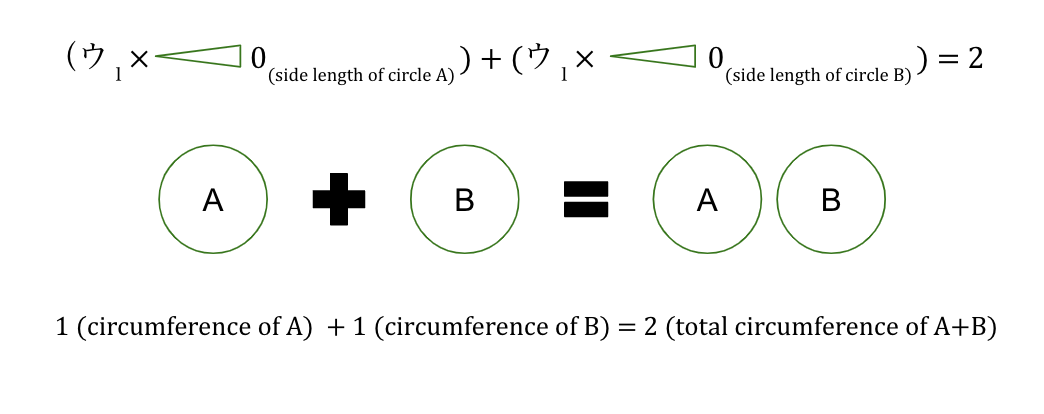
\includegraphics[width=1\linewidth]{Screenshot 2026-03-15 at 03.24.01.png}
    \caption{$(\text{\U}_1 \times 0_{\text{side of A}}) + 
    (\text{\U}_1 \times 0_{\text{side of B}}) = 2$. Two distinct circles, 
    each contributing a circumference of 1, for a total of 2. The two 
    zeroes are trivially distinct - one is the side length of circle A, 
    the other of circle B.}
    \label{fig:distributive-circles}
\end{figure}

When we write $(\text{\U}_1 \times 0) + (\text{\U}_1 \times 0) = 2$, 
we are not summing two identical expressions. We are asking two separate 
instruction codes to each produce a circle - circle $A$ and circle $B$ - 
and summing their circumferences. The two zeroes are trivially distinct: 
one is the side length of $A$, the other the side length of $B$. They 
are not interchangeable.\\\\
Although $0 + 0 = 0$ is true, these zeroes are contextually defined as being the side length edges (or ``zero triangles") still carry 
trivial data that cannot be discarded. Adding them doesn't erase the information they contain, and the fact that they represent different sides of different circles. Instead it produces a zero carrying the \textbf{concatenated trivial 
data} of both side lengths:
$$0_{\text{side of A}} + 0_{\text{side of B}} = 0_{\text{side of A and B}}$$This concatenated zero, when read by \U$_1$, will instructs it to produce 
\textit{both} circles simultaneously - which is exactly the correct 
result:
$$\text{\U}_1 \times 0_{\text{side of A and B}} = 2 \quad \checkmark$$The distributive law is not violated. It holds - but only when the 
trivial labels are carried through correctly. The apparent contradiction 
arose from stripping the trivial data from the zeroes and treating them 
as interchangeable. \textbf{In this framework, zeroes are not 
interchangeable unless their trivial data matches.}

\subsubsection*{Other Algebraic Problems}

The following addresses remaining algebraic edge cases that arise when 
manipulating division by zero expressions.

\subsubsection*{Problem 3: $\frac{1}{0} \times k = \frac{k}{0}$}

This holds when $k$ carries the trivial label of a \textbf{scale factor}. 
Since \U{} is a geometric instruction code, a scale factor updates the 
code rather than performing arithmetic on it:
$$\text{\U}_C \times k_{\text{scale}} = \text{\U}_{kC} = \frac{kC}{0}$$
However, if $k$ is instead redefined as $k = \frac{1}{n}$ for some 
$n \neq 0$, the result depends entirely on the trivial label of $k$. 
If $k$ carries a scale label, the redefinition updates the code 
regardless of how $k$ is expressed. If $k$ is \textbf{arbitrary} 
(no scale label), the operation does not change the virtual data of 
\U{} at all, since by actuality $\infty \times k = \infty$ for any 
finite $k$.

\subsubsection*{Problem 4: $\frac{1}{0} + \frac{1}{0} = \frac{2}{0}$?}

This expression is \textbf{meaningless}. Addition is a directional 
operation and has no effect on \U{}: literally adding \U{} to itself 
does not change its geometric instruction code from \U$_1$ to \U$_2$. 
The only operation that updates the code is scaling:
$$\text{\U}_C \times 2_{\text{scale}} = \text{\U}_{2C}$$
Addition of \U{} expressions is undefined and produces no result.

\subsubsection*{Problem 5: $\frac{1}{0} - \frac{1}{0} = 0$?}

This expression is \textbf{meaningless} but not entirely wrong. In this 
number system, $\infty - \infty$ is undefined when the two infinities 
carry arbitrary or non-matching virtual data, exactly the same as the indeterminate property of infinity. However, if both \U{} expressions carry 
\textbf{strictly matching} virtuality, the subtraction \textit{could} 
produce $0$, since the codes cancel. If the virtualities differ in any 
way, the expression remains undefined.

\subsubsection*{Problem 6: $\frac{1}{0} = \frac{2}{0}$?}

\textbf{True by actuality, false by virtuality.} Since both expressions 
have actual value $\infty$:
$$\frac{1}{0} = \frac{2}{0}$$
$$\text{\U}_1 \ _a{=}{}_a \ \text{\U}_2$$
But virtually they are entirely distinct instruction codes:
$$\text{\U}_1 \ {}_v{\neq}{}_v \ \text{\U}_2$$

\subsubsection*{Problem 7: $\frac{1}{0} \times 0 = \frac{2}{0} \times 0 \implies1=2$?}

Ironically, this is not really an issue in this number system. The 
explanation is straightforward: despite being an actual equality, 
$\frac{1}{0}$ and $\frac{2}{0}$ are completely virtually distinct, with  
one carrying the instruction code of a circle of circumference $C = 1$, and  
the other of $C = 2$. It is \textbf{virtuality}, not \textbf{actuality}, 
that defines the algebraic behavior of these expressions. So the 
equation producing an apparent contradiction is not inherently \textit{wrong}, because
both sides are \textbf{actually equal} but are also \textbf{virtually different}, 
and it is the virtual data that governs the outcome.
\\\\This mirrors the behaviour of sub-infinitesimal data established in 
Chapter 5. A zero initialized with sub-infinitesimal data can produce 
non-zero results:
$$0_{[0.5\varepsilon_\Omega]} \times 2 = \varepsilon_\Omega$$
even though traditionally $0 \times 2 = 0$. This is not a contradiction, as although $0 = 0_{[0.5\varepsilon_\Omega]}$ by actuality, the two 
expressions are virtually distinct, and it is virtuality that governs algebraic
behavior. Actual equality does not imply virtual equality, and this 
principle applies throughout the framework.

\subsubsection{Defining $\frac{0}{0}$}

So far, division by zero has been defined for any \textbf{nonzero} 
numerator, in the form $\frac{C}{0} =_v \text{\U}_C$. The case 
$\frac{0}{0}$ has not yet been addressed, however, extending the geometric definition yields a direct answer. Recall 
that under geometric and trivial labelling:
$$\frac{C}{0} \times k_{\text{scale}} = \frac{kC}{0}$$
When $k = 0$, we are scaling a circle by zero: annihilating it 
completely. A circle scaled to circumference zero is not a circle at 
all: it is a point. Since a point has no edges, and division by zero 
is in part virtually defined as the ``side count" of a virtual circle, we conclude that $\text{\U}_0 = 0$ because a point \textbf{has no sides}.

\begin{figure}[H]
    \centering
    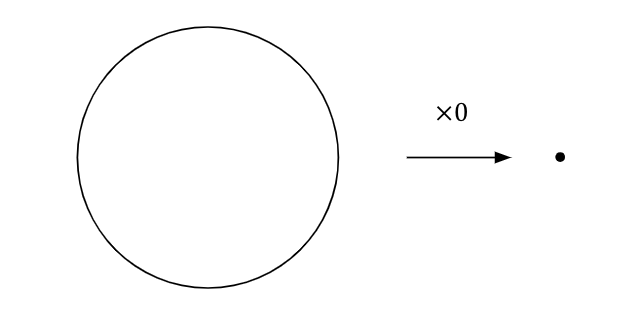
\includegraphics[width=0.7\linewidth]{Screenshot 2026-03-14 at 23.25.08.png}
    \caption{A circle scaled by factor zero becomes a point. \U$_0 = 0$ 
    follows directly from the geometric definition: a circle of 
    circumference zero has no sides and no structure.}
    \label{fig:circle-to-point}
\end{figure}

This result is not merely asserted, but is a direct consequence of 
the definition. It is also consistent with the following independent 
argument by contradiction. Suppose $\frac{0}{0} = k$ for some 
$k \neq 0$. Then:
\begin{align*}
0 \times 1 &= 0 \times 17 \\[6pt]
\dfrac{0 \times 1}{0} &= \dfrac{0 \times 17}{0} \\[6pt]
k \times 1 &= k \times 17 \\[6pt]
k &= 17k
\end{align*}
This is only satisfied when $k = 0$, contradicting the assumption. 
Therefore $\frac{0}{0} = 0$.\footnote{This argument is presented by 
blackpenredpen \cite{bprp_zerodzero}.} Although the argument assumes 
that dividing both sides by zero is valid, which is something traditional 
mathematicians would contest. However, within this framework, where division 
by zero is defined, it holds. The convergence of two independent 
approaches onto the same answer is a satisfying confirmation.
\\\\\U$_0 = 0$ is therefore the \textbf{geometric definition} of 
$\frac{0}{0}$: clean, context-dependent, and a direct consequence of 
the circle definition. It is worth noting that $\frac{0}{0}$ remains fundamentally 
indeterminate outside this geometric context, since $0 \times k = 0$ 
for all $k$, stripping away the trivial labeling leaves the expression 
without a determinate value. Within the framework however, a further 
definition arises naturally from sub-infinitesimal data, in which both 
zeroes in $\frac{0}{0}$ are initialized by sub-infinitesimal expressions. 
This definition underlies the replacement of the classical limit in 
$\mathbb{R}_\Omega$, and is covered in Chapter 10.

\section{Conclusion}

We began this theory with a philosophical concept: the idea that different 
absences of objects are metaphysically distinct. That in some philosophical 
manner, the absence of apples and the absence of bananas could be 
distinguished despite both being ``nothing''. It was an abstract idea, and 
one traditionally unrelated to mathematics. Yet we chose to develop it, and 
find a way to re-imagine it in a more mathematical manner. From this bizarre 
abstract concept came the entire cornerstone of this theory: \textbf{mathematical 
data} (or ``meta''-data), which is the actualisation of this philosophical concept 
into mathematics: the idea that numbers can carry qualitative information 
beyond their actual values.
\\\\Although seemingly pointless, we continued from this philosophical foundation, 
developing and constructing a new number system, which we called the absolute 
hyper-reals: $\mathbb{R}_\Omega$. The absolute hyper-reals were a re-imagining of the 
hyperreals with \textbf{two} radical departures from the standard hyper-reals and mathematical conventions as a whole.
\\\\The first is that it is not a purely continuous number system. Despite being 
a superset of the reals, which \textit{are} continuous, the absolute 
hyper-reals are not. The reals function only as a small continuous sub-region 
embedded into a larger \textbf{discrete} structure: bounded below by the 
absolute infinitesimal $\varepsilon_\Omega$, the smallest nonzero magnitude, 
and above by its reciprocal, the absolute hyperfinite $\omega_\Omega$, the 
largest finite magnitude. Above and below these bounds we encounter infinity 
and zero, each with a reciprocal relationship to the other, defining the 
identity $\frac{1}{0} = \infty$ in $\mathbb{R}_\Omega \cup \infty$.
\\\\This number system came with particularities, because we also reinterpreted 
what lies beyond these bounds as not merely being ``zero'' or ``infinity'', but as being zero and infinity through the lens of \textbf{mathematical data}. Zero was conceptually extended to comprise of \textbf{zero-equivalent 
sub-infinitesimal data} whilst infinity was likewise also extended to comprise of \textbf{specific infinite data}. This distinction 
between the actuality and virtuality of numbers became the \textit{core} of the 
framework. It fundamentally reinterpreted continuity, and enabled an 
\textbf{invertibility} of zero and infinity: where actuality collapses, 
data persists. Sub-infinitesimal data allowed for expressions falling below the lower bound of actuality to recover it's lost magnitude through multiplication. Likewise, specific infinite 
data allows infinity to return to finiteness. 
\\\\These different sub-infinitesimal and specific infinite data expressions, 
despite coming in an infinite variety of flavours, all share the same actual 
value while differing in virtual data, decoupling numerical magnitude from 
algebraic behaviour, and cementing $\frac{1}{0} = \infty$ as an identity.
\\\\However, this definition of division by zero, in which $\frac{1}{0} = \infty$ was only valid \textit{conditionally} - when zero carried sub-infinitesimal data. Without this condition, the traditional definition of zero with 
its annihilator property still remained undefined as a divisor. At least, algebraically 
it was. The solution lay in geometry.
\\\\Interpreting geometry through the lens of $\mathbb{R}_\Omega$ is fundamentally 
different from continuous $\mathbb{R}$-derived geometry, as the lower bound of 
magnitude produces a lower bound for area, $\sqrt{\varepsilon_\Omega}$, making it so geometrical figures collapsed at certain thresholds. This necessitated a \textit{third} manifestation of mathematical data, which extended the principles of mathematical data to geometry itself: where physical figures collapse below the atomic 
thresholds of $\mathbb{R}_\Omega^2$, their structural identity persists 
virtually.
\\\\We then proceeded to utilize this concept to define curvature and circularity, as true curvature is fundamentally physically impossible in $\mathbb{R}_\Omega^2$, due to the fact that physically everything is pixilated and flattened, making it so traditionally curved figures become discrete near the atomic threshold. 
\\\\The solution to this problem of defining circles was to utilize geometric data, and define a circle not as a physical structure but as a virtual one, in which a circle was virtually defined as being a regular polygon of side length 
$0$ and side count $\frac{C}{0}$, \textit{encoded} inside a physical structure. Despite the absurdity of the claim, it worked 
mathematically: a polygon of virtual side length zero does not scale its edges, 
keeping them atomically smooth, while allowing the circumference to grow.
\\\\This gave us the definition of division by zero as a \textit{specific infinite 
data} of infinity: a virtuality that infinity can possess, acting as a code 
which enables curvature in $\mathbb{R}_\Omega^2$. From this, we defined \U{}, 
we defined $\frac{0}{0}$, and we addressed the algebraic consistency of the 
framework through trivial data, solving what this paper set out to solve - division by zero. Although this paper isn't fully done yet, as there is an extra chapter after this conclusion covering the application of the concepts of this paper to \textit{calculus}, serving as the basis to "new" nonstandard analysis, the conceptual ideas behind this framework have been talked and introduced, and I believe that concluding the theory here is appropriate.
\\\\Before we move on, I would like to take another less-than-formal second to make a few statements.
\\\\I do not claim this framework is fully completed or mathematically rigorous. As a matter of fact, I would claim that this theory is currently vastly \textbf{incomplete}, and requires a lot of work and development for it to gain completeness, rigor and legitimacy. If this theory were to be ``accepted'' by the mathematical community, which is already a big idealization, future work and development of the ideas present in this theory are not just a proposition but a necessity in order to achieve formalization.
\\\\However, I wouldn't sell myself short either. Despite the naiveness and potential wrongness of my ideas, I do believe there is something here. Although this isn't a completed number system, I would say that the contents of this paper may potentially serve as the conceptual and speculative base for an actually \textit{good} number system.
\\\\I still find myself very proud of the completion and actualization of my ideas in this work. My naive wish above all else is to see my ideas potentially evolve and serve someone in the future. Even if this theory isn't perfect, after all this hard work and countless hours of effort, I can at least proudly say that this theory is at the very least \textit{coherent}. It expresses my ideas and inner naiveness about the subject accurately, and that is honestly everything I could ever ask for. With this in mind, let us proceed to the final chapter: the application of this theory to calculus, and the foundation of what I call ``new'' nonstandard analysis.

\newpage
\section{Chapter 10 - Calculus in $\mathbb{R}_\Omega$}

This work, though heavily inspired by nonstandard analysis, was never constructed to be a practical number system. Its creation served a singular purpose: defining division by zero. In every sense, $\mathbb{R}_\Omega$ is a ``fan number system'' built from curiosity, not necessity.\\Yet in adapting calculus to this framework, something unexpected emerged. Not only does calculus \textit{work} in $\mathbb{R}_\Omega$, but it refines it into something genuinely usable. What began as a niche construction for encoding curvature through division by zero has become a coherent calculus framework. Despite its naive origins, $\mathbb{R}_\Omega$ may offer advantages over standard hyperreals: it allows direct assertions without requiring the standard part function.

\subsection{The Limit Reconsidered}

To understand $\mathbb{R}_\Omega$, one must first understand its philosophical departure from classical limits.\\In standard calculus, a limit evaluates behavior as a function approaches, but never reaches, a value. The limit of $f(x)$ as $x \to c$ analyzes how $f(x)$ behaves when $x$ gets arbitrarily close to $c$, without ever equaling $c$.\\\\Consider the classic example: $f(x) = \frac{1}{x}$. In real calculus, $f(0)$ is undefined.

\begin{figure}[H]
    \centering
    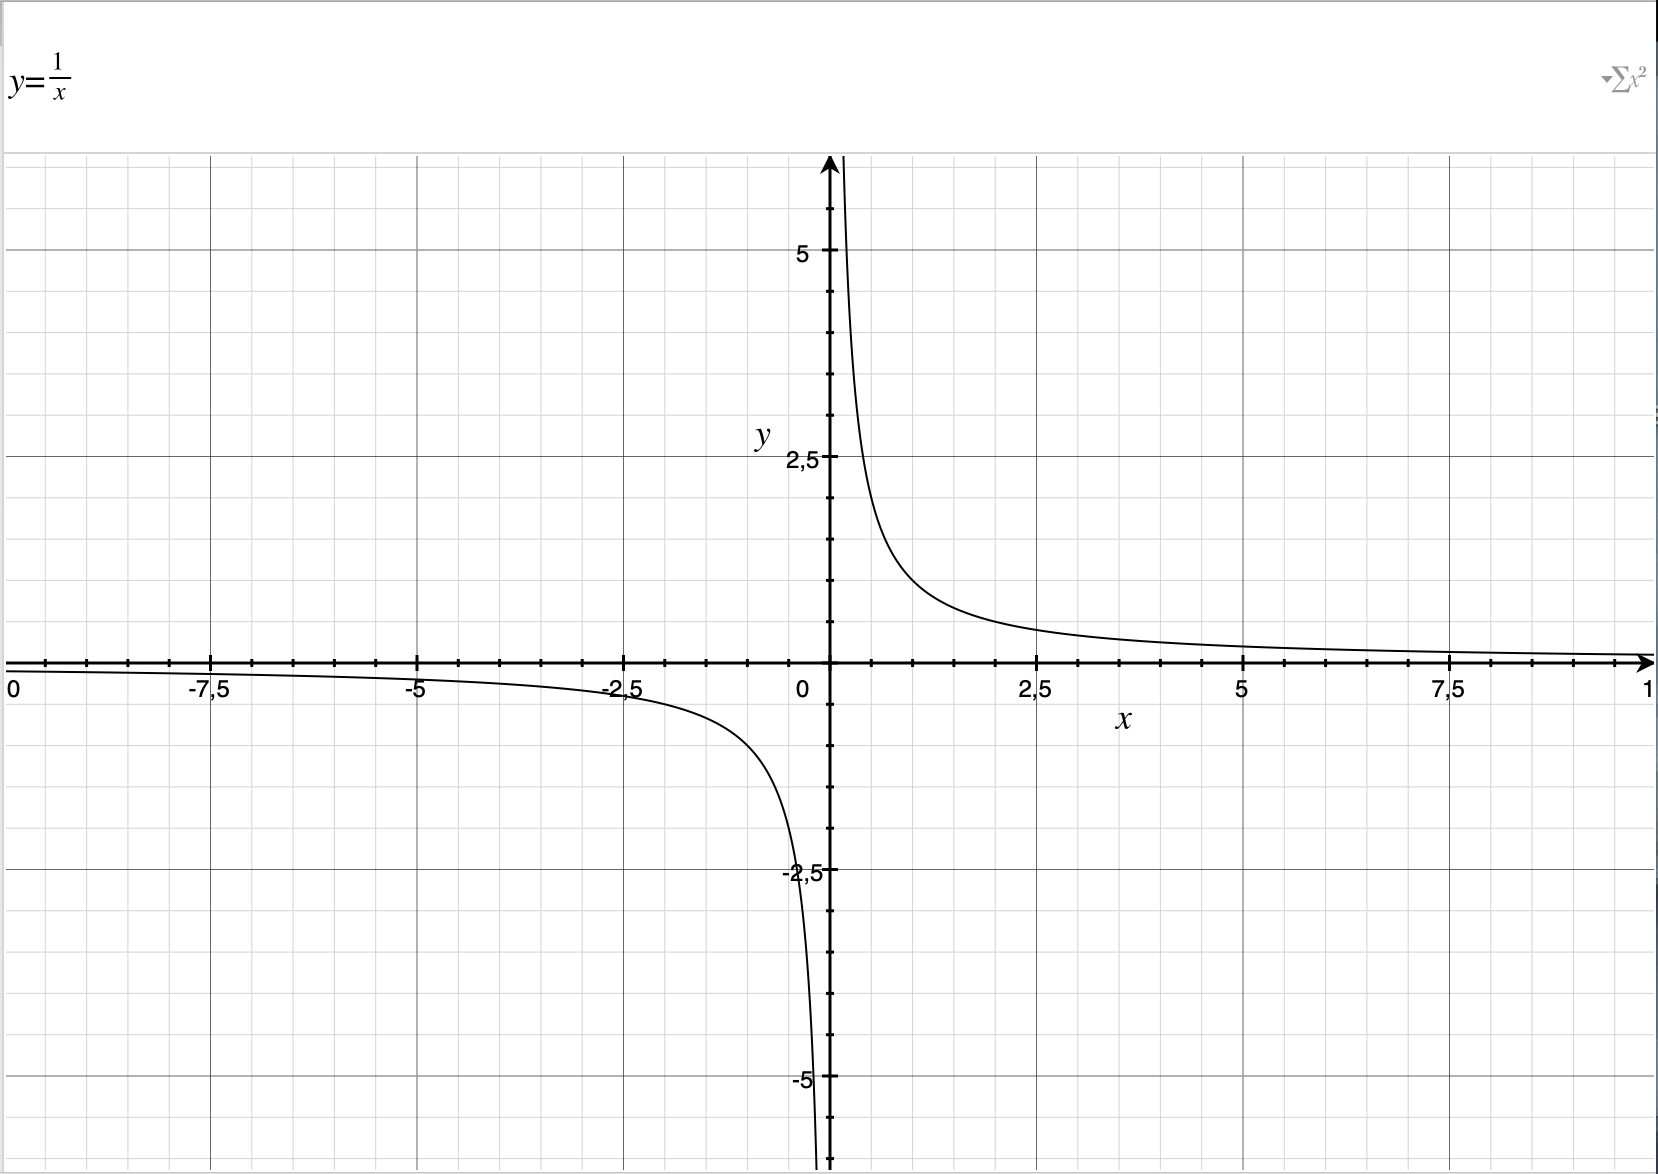
\includegraphics[width=1\linewidth]{Screenshot 2026-02-28 at 22.25.33.png}
    \caption{The function $f(x) = \frac{1}{x}$}
    \label{fig:reciprocal-function}
\end{figure}Taking the limit as $x \to 0^+$ (approaching from the right), we observe that as $x$ decreases toward zero, $f(x)$ increases without bound. Plugging in values like $x = 0.1, 0.01, 0.001$ yields $f(x) = 10, 100, 1000$, indicating that the function diverges to infinity.
\\\\Formally:
$$\lim_{x \to 0^+} \frac{1}{x} = \infty$$\\This does not mean $f(0) = \infty$. It means $f(x)$ grows without bound as $x$ approaches zero from the right.\\In hyper-real non-standard analysis (Robinson), limits are replaced by infinitesimal reasoning. Instead of approaching zero, we evaluate $f$ at an infinitesimal distance ($\varepsilon$) from our chosen point (0 in this case):
$$f(\varepsilon) = \frac{1}{\varepsilon} = \omega$$\\where $\omega$ is a hyperfinite (infinite) number. The standard part function then extracts the real value:
$$\text{st}(\omega) = \infty \quad \text{(divergence)}$$\\In $\mathbb{R}_\Omega$, we go further than that, as with the inclusion of absolute elements and mathematical metadata, we are able to evaluate functions at zero-equivalent or absolute infinitesimal values \textbf{directly} without limits and without the standard part function. 

This is possible through two distinct approaches:

\begin{itemize}
\item \textbf{Asymmetric evaluation:} We evaluate \textit{asymmetrically} using virtuality (sub-infinitesimal and specific infinite data).
\item \textbf{Symmetric evaluation:} We evaluate \textit{symmetrically} using actuality (absolute infinitesimal and hyperfinite).
\end{itemize}

\subsubsection{Asymmetric Evaluation (Virtual Evaluation)}

To evaluate $f(x)$ at $x = 0$ asymmetrically, we use a \textbf{zero-equivalent virtual value}—a sub-infinitesimal data expression $0_{[n\varepsilon_\Omega]}$ where $|n| < 1$.\\Since $n\varepsilon_\Omega < \varepsilon_\Omega$, the value is zero-equivalent. We substitute this virtual zero into the function, evaluate it using virtual arithmetic, then convert it to actual notation.

Let $h \to_v 0_{[n\varepsilon_\Omega]}$ be a zero-equivalent value. Then:
$$f(h) =_v \frac{1}{0_{[n\varepsilon_\Omega]}} =_v \infty_{[\frac{1}{n}\omega_\Omega]}$$

By actuality:
$$f(0) = \infty$$

\textbf{Example:} For $h \to_v 0_{[0.1\varepsilon_\Omega]}$:
$$f(0_{[0.1\varepsilon_\Omega]}) =_v \frac{1}{0_{[0.1\varepsilon_\Omega]}} =_v \infty_{[10\omega_\Omega]}$$

Converting to actual value:
$$f(0) = \infty$$This approach mirrors classical limits but evaluates \textit{at} zero virtually, rather than approaching zero asymptotically.\\\\\textbf{Negative asymmetric evaluation:} Using $h \to_v 0_{[-0.1\varepsilon_\Omega]}$:
$$f(0_{[-0.1\varepsilon_\Omega]}) =_v \infty_{[-10\omega_\Omega]}$$\\By actuality, still:
$$f(0) = \infty$$\\Both positive and negative sub-infinitesimal approaches yield the same actual value, confirming the function diverges (is equal to infinity by actuality) at zero. Virtually, the result depends on the chosen sub-infinitesimal data: different sub-infinitesimal data of $h$ yield different specific infinite data. In this context, the \textbf{choice} of data is arbitrary, but the function is no longer simply 'undefined': it has a well-defined virtual expression for any given sub-infinitesimal input.

\subsubsection{Symmetric Evaluation (Actual Evaluation)}

Symmetric evaluation uses \textbf{actual absolute infinitesimals}, not virtual data. Instead of evaluating directly at a point, we sample the function symmetrically around the point, one step $\varepsilon_\Omega$ to the right, one step $\varepsilon_\Omega$ to the left and compare the results.

For $f(x) = \frac{1}{x}$ at $x = 0$:\\\textbf{Positive displacement:}
$$f(\varepsilon_\Omega) = \frac{1}{\varepsilon_\Omega} = \omega_\Omega$$\\\textbf{Negative displacement:}
$$f(-\varepsilon_\Omega) = \frac{1}{-\varepsilon_\Omega} = -\omega_\Omega$$\\Comparing: $\omega_\Omega \neq -\omega_\Omega$ and $\omega_\Omega \not\approx -\omega_\Omega$ (they are not infinitesimally close).\\Since the two values are not equal or approximately equal, we cannot take their average. The function fails symmetric evaluation - it is a special case in which the ``true'' value at zero cannot be determined via symmetric evaluations, and is uniquely defined solely through specific infinite data (\U$_1$ or $k\omega_\Omega$).\\\\This however, does confirm divergence, meaning the actual value is still $\infty$.

\subsubsection{Evaluating Removable Discontinuities}

Consider $f(x) = \frac{x^2 - 1}{x - 1}$, which is undefined at $x = 1$ (produces $\frac{0}{0}$).\\\\\textbf{Asymmetric evaluation:}

Let $h \to_v 0_{[n\varepsilon_\Omega]}$ be zero-equivalent. Evaluate at $x = 1 + h$:
$$f(1 + h) =_v \frac{(1 + h)^2 - 1}{(1 + h) - 1}$$

Expanding (suppressing virtuality notation for clarity):
$$f(1 + 0) =_v \frac{1 + 2h + h^2 - 1}{h} =_v \frac{2h + h^2}{h} =_v 2 + h$$

By actuality:
$$f(1) = 2$$\\\textbf{Symmetric evaluation:}

Positive displacement:
$$f(1 + \varepsilon_\Omega) = \frac{(1 + \varepsilon_\Omega)^2 - 1}{(1 + \varepsilon_\Omega) - 1} = \frac{1 + 2\varepsilon_\Omega + 0_{[\varepsilon_\Omega^2]} - 1}{\varepsilon_\Omega}$$
$$= \frac{2\varepsilon_\Omega + 0_{[\varepsilon_\Omega^2]}}{\varepsilon_\Omega} = 2+\varepsilon_\Omega$$Despite being a zero-equivalent term, the data $0_{[\varepsilon_\Omega^2]}$ \textit{does} have the property that $0_{[\varepsilon_\Omega^2]}\div{\varepsilon_\Omega}=\varepsilon_\Omega$, so it cannot be ignored.
Negative displacement:
$$f(1 - \varepsilon_\Omega) = \frac{(1 - \varepsilon_\Omega)^2 - 1}{(1 - \varepsilon_\Omega) - 1} = \frac{1 - 2\varepsilon_\Omega + 0_{[\varepsilon_\Omega^2]} - 1}{-\varepsilon_\Omega}$$
$$= \frac{-2\varepsilon_\Omega + 0_{[\varepsilon_\Omega^2]}}{-\varepsilon_\Omega} = 2-\varepsilon_\Omega$$Since $f(1 + \varepsilon_\Omega) \approx f(1 - \varepsilon_\Omega)$, then we can take the average of these two as the difference is only absolutely infinitesimal. Doing so yields the following:
$$\frac{2 +\varepsilon_\Omega+ 2-\varepsilon_\Omega}{2} = 2$$Giving us our symmetric evaluation of $f(1) = 2$.\\\\\textbf{Another example:} Symmetric evaluation of $f(x) = \frac{\sin(x)}{x}$ at $x = 0$.\\We choose a symmetric evaluation of trigonometric functions as they are simpler, as we can directly expand \textbf{Taylor series}.

The expansion of $\sin(x)$ is:
$$\sin(x) = x - \frac{x^3}{6} + \frac{x^5}{120} - \cdots$$For $x = \varepsilon_\Omega$:
$$\sin(\varepsilon_\Omega) = \varepsilon_\Omega - \frac{\varepsilon_\Omega^3}{6} + \cdots = \varepsilon_\Omega + 0_{[-\varepsilon_\Omega^3/6]} +\cdots= \varepsilon_\Omega$$Every term after the first two are zero-equivalent.
Thus, we very simply get that:
$$f(\varepsilon_\Omega) = \frac{\sin(\varepsilon_\Omega)}{\varepsilon_\Omega}=\frac{\varepsilon_\Omega}{\varepsilon_\Omega} = 1$$This however is only our first point, we also must take our second point $f(-\varepsilon_\Omega)$:

$$\sin(-\varepsilon_\Omega) = -\varepsilon_\Omega + \frac{\varepsilon_\Omega^3}{6} + \cdots = \varepsilon_\Omega + 0_{[\varepsilon_\Omega^3/6]}+0+0\cdots = -\varepsilon_\Omega$$

$$f(-\varepsilon_\Omega)=\frac{\sin(-\varepsilon_\Omega)}{-\varepsilon_\Omega}=1$$This symmetric evaluation around $f(0)$ give us the same value, so taking the average of the two yields:

$$\frac{f(\varepsilon_\Omega)+f(-\varepsilon_\Omega)}{2}=1$$Which matches the standard limit.

\subsection{The Derivative}

\subsubsection{The Classical Derivative}

The derivative by first principles is defined as:
$$f'(x) = \lim_{h \to 0} \frac{f(x+h) - f(x)}{h}$$This measures the \textbf{instantaneous rate of change} of $f$ at $x$. \\The numerator, $f(x+h) - f(x)$, is the change in output (vertical change). The denominator, $h$, is the change in input (horizontal change). The quotient:
$$\frac{f(x+h) - f(x)}{h}$$is the \textbf{difference quotient}, which is the average rate of change between $x$ and $x + h$.\\As $h \to 0$, this average becomes the instantaneous rate of change: the derivative.\\In hyperreal analysis (Robinson), the limit is replaced by evaluating at an infinitesimal $\varepsilon$:
$$f'(x) = \text{st}\left(\frac{f(x + \varepsilon) - f(x)}{\varepsilon}\right)$$The standard part function extracts the real value.\\In $\mathbb{R}_\Omega$, we define derivatives without limits or standard functions, using the similar two approaches as for the evaluation at a point:

\begin{itemize}
\item \textbf{Asymmetric derivative (virtual):} Uses sub-infinitesimal data
\item \textbf{Symmetric derivative (actual):} Uses absolute infinitesimals
\end{itemize}

\subsubsection{Asymmetric Derivative (Virtual Derivative)}

The asymmetric derivative directly translates the limit definition into virtual evaluation:
$$f'(x) =_v \frac{f(x + h) - f(x)}{h}, \quad \text{where } h \to_v 0_{[n\varepsilon_\Omega]}$$ Since $h$ is zero-equivalent ($h < \varepsilon_\Omega$), $x$ and $x + h$ are physically indistinguishable. The derivative is evaluated virtually, then converted to actual notation.\\\\\textbf{Example:} Differentiate $f(x) = x^2$ asymmetrically.

Let $h \to_v 0_{[n\varepsilon_\Omega]}$:
$$f'(x) =_v \frac{(x + h)^2 - x^2}{h} =_v \frac{x^2 + 2xh + h^2 - x^2}{h} =_v \frac{2xh + h^2}{h} =_v 2x + h$$By actuality, since $h$ is zero equivalent, this simply translates to:
$$f'(x) = 2x$$The asymmetric derivative evaluates identically to a classical limit.

\subsubsection{Symmetric Derivative (Perfect Derivative)}

The symmetric derivative uses the \textbf{centered difference quotient}:
$$f'(x) = \frac{f(x + \varepsilon_\Omega) - f(x - \varepsilon_\Omega)}{2\varepsilon_\Omega}$$This samples the function symmetrically around $x$: one step $\varepsilon_\Omega$ to the right, one step $\varepsilon_\Omega$ to the left. The average of these two slopes gives the exact derivative at $x$.\\I also informally call this the ``\textit{perfect derivative}'' because:
\begin{itemize}
\item It uses actual, non-zero values (not virtual data)
\item It gives the derivative directly without simplification or standard functions
\item Despite using finite displacements, it yields exact results
\end{itemize}
\\Classical calculus approaches the derivative from one side (forward or backward). The symmetric derivative approaches from both sides simultaneously, hitting the derivative exactly in the middle.\\Moreover, much like symmetric evaluations about a point, it can be computed directly using series expansions with no limits required.

\subsection{Examples: Computing Symmetric Derivatives}

We now demonstrate the symmetric derivative by differentiating three functions.

\subsubsection{Example 1: Polynomial}

$$f(x) = x^3 + 2x^2 + 4x + 6$$

The symmetric derivative is:
$$f'(x) = \frac{f(x + \varepsilon_\Omega) - f(x - \varepsilon_\Omega)}{2\varepsilon_\Omega}$$

Expanding:
\begin{align*}
f(x + \varepsilon_\Omega) &= (x + \varepsilon_\Omega)^3 + 2(x + \varepsilon_\Omega)^2 + 4(x + \varepsilon_\Omega) + 6 \\
&= x^3 + 3x^2\varepsilon_\Omega + 3x\varepsilon_\Omega^2 + 0_{[\varepsilon_\Omega^3]} + 2x^2 + 4x\varepsilon_\Omega + 0_{[2\varepsilon_\Omega^2]} + 4x + 4\varepsilon_\Omega + 6
\\
f(x - \varepsilon_\Omega) &= (x - \varepsilon_\Omega)^3 + 2(x - \varepsilon_\Omega)^2 + 4(x - \varepsilon_\Omega) + 6 \\
&= x^3 
+ 2x^2  - 3\varepsilon_\Omega x^2 
+ 3\varepsilon_\Omega^2x - 4\varepsilon_\Omega x + 4x \\
&\quad - 0_{[\varepsilon_\Omega^3]} + 0_{[2\varepsilon_\Omega^2]} - 4\varepsilon_\Omega + 6
\end{align*}

Subtracting:
\begin{align*}
f(x + \varepsilon_\Omega) - f(x - \varepsilon_\Omega) &= 6x^2\varepsilon_\Omega + 0_{[2\varepsilon_\Omega^3]}  + 8x\varepsilon_\Omega + 8\varepsilon_\Omega
\end{align*}

Dividing by $2\varepsilon_\Omega$:
$$f'(x) = 3x^2 + 0_{[\varepsilon_\Omega^2]} + 4x + 4$$

Since $\varepsilon_\Omega^2 = 0$ (zero-equivalent):
$$f'(x) = 3x^2 + 4x + 4$$

This matches the standard derivative.

\subsubsection{Example 2: Exponential Function}

$$f(x) = xe^x$$

The symmetric derivative is:
$$f'(x) = \frac{(x + \varepsilon_\Omega)e^{x + \varepsilon_\Omega} - (x - \varepsilon_\Omega)e^{x - \varepsilon_\Omega}}{2\varepsilon_\Omega}$$

We expand $e^{\varepsilon_\Omega}$ using the Taylor series:
$$e^y = 1 + y + \frac{y^2}{2!} + \frac{y^3}{3!} + \cdots$$

For $y = \varepsilon_\Omega$:
$$e^{\varepsilon_\Omega} = 1 + \varepsilon_\Omega + \frac{\varepsilon_\Omega^2}{2} + \cdots$$

Since $\varepsilon_\Omega^2 = 0$, we keep only the first two terms:
$$e^{\varepsilon_\Omega} = 1 + \varepsilon_\Omega$$

Then:
\begin{align*}
(x + \varepsilon_\Omega)e^{x + \varepsilon_\Omega} &= (x + \varepsilon_\Omega)e^x e^{\varepsilon_\Omega} \\
&= (x + \varepsilon_\Omega)e^x(1 + \varepsilon_\Omega) \\
&= (x + \varepsilon_\Omega)e^x + (x + \varepsilon_\Omega)e^x\varepsilon_\Omega
\end{align*}

Similarly:
\begin{align*}
(x - \varepsilon_\Omega)e^{x - \varepsilon_\Omega} &= (x - \varepsilon_\Omega)e^x(1 - \varepsilon_\Omega)
\end{align*}

Subtracting:
\begin{align*}
&(x + \varepsilon_\Omega)e^x(1 + \varepsilon_\Omega) - (x - \varepsilon_\Omega)e^x(1 - \varepsilon_\Omega) \\
&= xe^x+\varepsilon_\Omega xe^x+\varepsilon_\Omega e^x+\varepsilon_\Omega^2e^x-xe^x
+\varepsilon_\Omega xe^x+\varepsilon_\Omega e^x-\varepsilon_\Omega^2 e^x=2xe^x\varepsilon_\Omega + 2e^x\varepsilon_\Omega
\end{align*}

Dividing by $2\varepsilon_\Omega$:
$$f'(x) = xe^x + e^x$$

This matches the standard derivative.

\subsubsection{Example 3: Cube Root of Polynomial}

$$f(x) = \sqrt[3]{x^2 + 2}$$

The symmetric derivative is:
$$f'(x) = \frac{\sqrt[3]{(x + \varepsilon_\Omega)^2 + 2} - \sqrt[3]{(x - \varepsilon_\Omega)^2 + 2}}{2\varepsilon_\Omega}$$

Expanding the squared terms completely:
\begin{align*}
(x + \varepsilon_\Omega)^2 + 2 &= x^2 + 2x\varepsilon_\Omega + \varepsilon_\Omega^2 + 2 \\
(x - \varepsilon_\Omega)^2 + 2 &= x^2 - 2x\varepsilon_\Omega + \varepsilon_\Omega^2 + 2 
\end{align*}

In zero-equivalent notation:
\begin{align*}
(x + \varepsilon_\Omega)^2 + 2 &= x^2 + 2x\varepsilon_\Omega + 0_{[\varepsilon_\Omega^2]} + 2 \\
(x - \varepsilon_\Omega)^2 + 2 &= x^2 - 2x\varepsilon_\Omega + 0_{[\varepsilon_\Omega^2]} + 2 
\end{align*}

Let $A = x^2 + 2 + 0_{[\varepsilon_\Omega^2]}$ (keeping the zero-equivalent term explicitly):
$$f'(x) = \frac{\sqrt[3]{A + 2x\varepsilon_\Omega} - \sqrt[3]{A - 2x\varepsilon_\Omega}}{2\varepsilon_\Omega}$$

Factor out $A^{1/3}$:
$$f'(x) = \frac{A^{1/3}\left[\left(1 + \frac{2x\varepsilon_\Omega}{A}\right)^{1/3} - \left(1 - \frac{2x\varepsilon_\Omega}{A}\right)^{1/3}\right]}{2\varepsilon_\Omega}$$

Now we expand using the binomial series, keeping the first \textbf{three} terms:
$$(1 + y)^{1/3} = 1 + \frac{1}{3}y - \frac{1}{9}y^2 + \frac{5}{81}y^3 - \cdots$$

For $y = \frac{2x\varepsilon_\Omega}{A}$:

\textbf{Positive term:}
\begin{align*}
\left(1 + \frac{2x\varepsilon_\Omega}{A}\right)^{1/3} &= 1 + \frac{1}{3}\left(\frac{2x\varepsilon_\Omega}{A}\right) - \frac{1}{9}\left(\frac{2x\varepsilon_\Omega}{A}\right)^2 + \cdots \\
&= 1 + \frac{2x\varepsilon_\Omega}{3A} - \frac{1}{9} \cdot \frac{4x^2\varepsilon_\Omega^2}{A^2} + \cdots \\
&= 1 + \frac{2x\varepsilon_\Omega}{3A} + 0_{[-4x^2\varepsilon_\Omega^2/9A^2]}
\end{align*}

\textbf{Negative term:}
\begin{align*}
\left(1 - \frac{2x\varepsilon_\Omega}{A}\right)^{1/3} &= 1 - \frac{1}{3}\left(\frac{2x\varepsilon_\Omega}{A}\right) - \frac{1}{9}\left(\frac{2x\varepsilon_\Omega}{A}\right)^2 - \cdots \\
&= 1 - \frac{2x\varepsilon_\Omega}{3A} - \frac{1}{9} \cdot \frac{4x^2\varepsilon_\Omega^2}{A^2} - \cdots \\
&= 1 - \frac{2x\varepsilon_\Omega}{3A} + 0_{[-4x^2\varepsilon_\Omega^2/9A^2]}
\end{align*}

Subtracting the two expansions:
\begin{align*}
&\left(1 + \frac{2x\varepsilon_\Omega}{3A} + 0_{[-4x^2\varepsilon_\Omega^2/9A^2]}\right) - \left(1 - \frac{2x\varepsilon_\Omega}{3A} + 0_{[-4x^2\varepsilon_\Omega^2/9A^2]}\right) \\
&= \frac{2x\varepsilon_\Omega}{3A} + \frac{2x\varepsilon_\Omega}{3A} + 0_{[-4x^2\varepsilon_\Omega^2/9A^2]} - 0_{[-4x^2\varepsilon_\Omega^2/9A^2]} \\
&= \frac{4x\varepsilon_\Omega}{3A} + 0
\end{align*}

\textbf{Notice}: The $\varepsilon_\Omega^2$ terms cancel.

Continuing:
$$f'(x) = \frac{A^{1/3} \cdot \frac{4x\varepsilon_\Omega}{3A}}{2\varepsilon_\Omega}$$

Simplifying:
$$f'(x) = \frac{A^{1/3} \cdot 4x\varepsilon_\Omega}{3A \cdot 2\varepsilon_\Omega} = \frac{4x}{6A^{2/3}} = \frac{2x}{3A^{2/3}}$$

Now substitute $A = x^2 + 2 + 0_{[\varepsilon_\Omega^2]}$:
$$f'(x) = \frac{2x}{3(x^2 + 2 + 0_{[\varepsilon_\Omega^2]})^{2/3}}$$

Since $0_{[\varepsilon_\Omega^2]}$ is zero-equivalent:
$$(x^2 + 2 + 0_{[\varepsilon_\Omega^2]})^{2/3} = (x^2 + 2)^{2/3}$$

Therefore:
$$f'(x) = \frac{2x}{3(x^2 + 2)^{2/3}}$$

This matches the standard derivative.

\subsubsection{Note on keeping higher-order terms}

Ultimately, whether one chooses to keep zero-equivalent terms with powers higher than 2 (which is technically the ``proper'' method) or immediately discard them does not affect the final answer. All such terms vanish in the final result because the symmetric derivative is, by design, self-correcting.\\The centered difference quotient forces a structural cancellation pattern:
\begin{itemize}
\item \textbf{Odd-power terms} (like $\varepsilon_\Omega$, $\varepsilon_\Omega^3$, $\varepsilon_\Omega^5$, etc.) have opposite signs in $f(x + \varepsilon_\Omega)$ and $f(x - \varepsilon_\Omega)$, so they \textit{add} when subtracted
\item \textbf{Even-power terms} (like $\varepsilon_\Omega^2$, $\varepsilon_\Omega^4$, etc.) have the same sign in both expansions, so they \textit{cancel} when subtracted
\end{itemize}Among the surviving odd-power terms, only $\varepsilon_\Omega^1$ contributes to the final result. Higher odd powers ($\varepsilon_\Omega^3$, $\varepsilon_\Omega^5$, etc.) are divided by $2\varepsilon_\Omega$, leaving $\varepsilon_\Omega^2$, $\varepsilon_\Omega^4$, etc.—all zero-equivalent.\\\\The symmetric derivative automatically eliminates all error terms through its symmetry. This is why it produces exact results without requiring a standard part function or manual cleanup of infinitesimals.

\subsubsection{Additional Exercises}\\\\For fun, I recommend trying to differentiate these different functions symmetrically using absolute infinitesimals:

$$f(x)=\ln(x^2)$$ $$f(x)=\sin(x)e^x$$ $$f(x)=\tan(x^2)$$ 

\subsection{Integration in $\mathbb{R}_\Omega$}

Just as differentiation measures instantaneous rate of change, integration measures accumulated quantity. Most commonly, it measures the area under a curve.\\In classical calculus, integration is defined through \textbf{Riemann sums}, which is a simple idea: finding the area under a function $f(x)$ from $x = a$ to $x = b$. We achieve this by dividing the interval into small rectangles, computing the area of each rectangle, and then summing them all.

\begin{figure}[H]
    \centering
    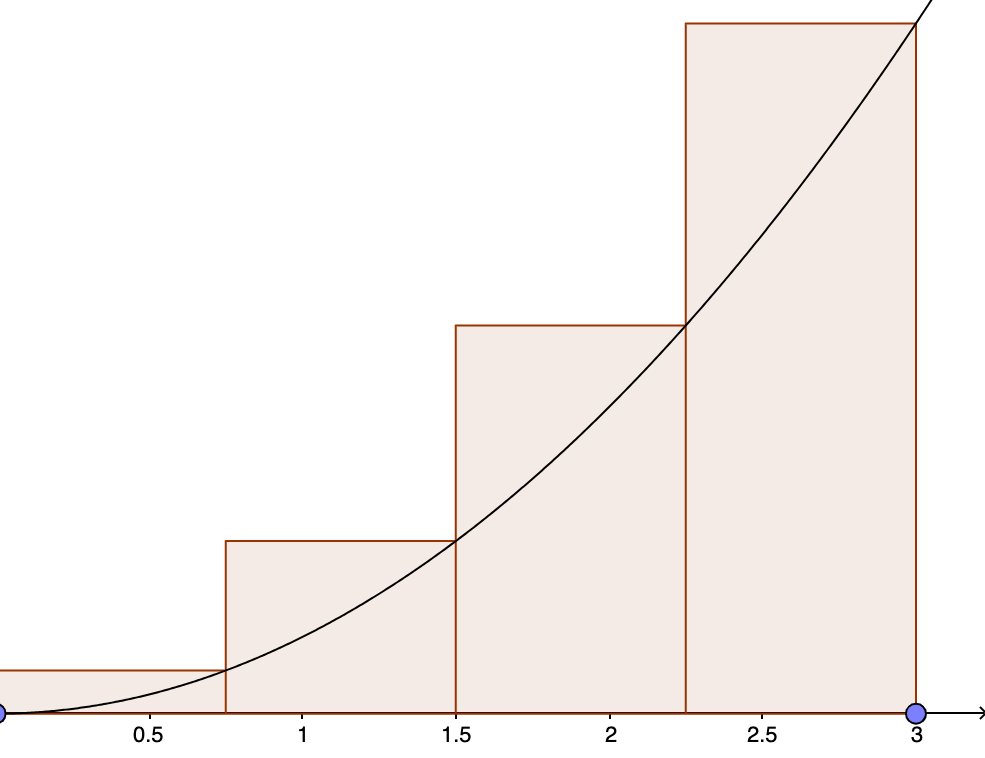
\includegraphics[width=0.5\linewidth]{Screenshot 2026-03-03 at 00.23.44.png}
    \caption{Riemann sum approximation of area under $f(x)$. The interval $[a,b]$ is divided into $n$ subintervals of width $\Delta x$.}
    \label{fig:riemann-sum}
\end{figure}

Each rectangle has:
\begin{itemize}
\item \textbf{Width:} $\Delta x$ (the size of each subinterval)
\item \textbf{Height:} $f(x_i)$ (the value of the function at some point in the subinterval)
\end{itemize}The area of one rectangle is $f(x_i) \cdot \Delta x$. Summing over all $n$ rectangles gives the total approximate area:
$$\text{Area} \approx \sum_{i=1}^{n} f(x_i) \Delta x$$The choice of where to sample the height $f(x_i)$ gives rise to three standard methods:

\textbf{Left Riemann Sum:} Sample at the left endpoint of each subinterval.
$$\sum_{i=0}^{n-1} f(x_i) \Delta x$$

\textbf{Right Riemann Sum:} Sample at the right endpoint of each subinterval.
$$\sum_{i=1}^{n} f(x_i) \Delta x$$

\textbf{Midpoint Riemann Sum:} Sample at the center of each subinterval.
$$\sum_{i=1}^{n} f\left(\frac{x_{i-1} + x_i}{2}\right) \Delta x$$As $n$ increases (making $\Delta x$ smaller), the approximation improves. In the limit as $n \to \infty$ (equivalently, $\Delta x \to 0$), the Riemann sum converges to the exact area—the definite integral:
$$\int_a^b f(x) \, dx = \lim_{n \to \infty} \sum_{i=1}^{n} f(x_i) \Delta x$$\\\textbf{In Standard Nonstandard Analysis:}\\\\In Robinson's framework, instead of taking a limit, we use an infinitesimal width $dx$ and sum over a hyperfinite number of rectangles. The integral is the standard part of this hyperfinite sum:
$$\int_a^b f(x) \, dx = \text{st}\left(\sum_{i=1}^{N} f(x_i) dx\right)$$where $N$ is hyperfinite (larger than any finite number but not infinite) and $dx = \frac{b-a}{N}$ is infinitesimal.The left, right, and midpoint sums still exist, but all three give the same standard part for continuous functions, thereby eliminating the need to specify which sampling method is used.\\In $\mathbb{R}_\Omega$, much like as we defined asymmetric and symmetric derivatives, we also define virtual and actual integrals, using virtual data and actual absolute infinitesimal and hyperfinite quantities.\\We define integration in two ways, mirroring our approach to differentiation:

\subsubsection{Asymmetric Integral (Left/Right Riemann Sum)}

The asymmetric integral uses a virtual sub-infinitesimal ``step length'' $d$ and specific infinite summation $\infty$:
$$d = \frac{b - a}{\infty}, \quad \text{where } \infty \to_v \infty_{[k\omega_\Omega]}$$

The only restriction: $\infty$ must make $d$ zero-equivalent ($d < |\varepsilon_\Omega|$).

The integral is:
$$\int_a^b f(x) \, dx =_v \sum_{i=1}^{\infty} f(x_i) d$$

\textbf{Example:} Integrate $f(x) = x + 3$ from $x = 1$ to $x = 3$ using virtuality.

Let $\infty \to_v \infty_{[k\omega_\Omega]}$ for some $k>>|1|$. Then:
$$d\to_v \frac{2}{\infty_{[k\omega_\Omega]}} =_v 0_{[2/k\omega_\Omega]}$$

$$x_i \to_v 1 + \frac{2i}{\infty_{[k\omega_\Omega]}}$$

$$\sum_{i=1}^{\infty_{[k\omega_\Omega]}} \left(1 + \frac{2i}{\infty_{[k\omega_\Omega]}} + 3\right) \cdot 0_{[2/k\omega_\Omega]}$$

$$=_v \sum_{i=1}^{\infty_{[k\omega_\Omega]}} \left(0_{[8/k\omega_\Omega]} + 0_{[4i/k^2\omega_\Omega^2]}\right)$$

Separating:
$$=_v 0_{[8/k\omega_\Omega]} \cdot \infty_{[k\omega_\Omega]} + 0_{[4/k^2\omega_\Omega^2]} \sum_{i=1}^{\infty_{[k\omega_\Omega]}} i$$

$$=_v 8 + 0_{[4/k^2\omega_\Omega^2]} \cdot \infty_{[\frac{k\omega_\Omega(k\omega_\Omega + 1)}{2}]}$$

$$=_v 8 + 2 + 0_{[2/k\omega_\Omega]}$$

By actuality,this gives:
$$\int_1^3 (x + 3) \, dx = 10$$Asymmetric integrals work but are less elegant than symmetric integrals due to the presence of infinite-equivalent and zero-equivalent expressions throughout the calculation. Symmetric integrals (midpoint rule with absolute infinitesimals) are preferred.

\subsubsection{Symmetric Integral (Midpoint Riemann Sum)}

Using absolute infinitesimal $\varepsilon_\Omega$ for rectangle width and absolute hyperfinite $\omega_\Omega$ for the number of rectangles, the symmetric integral employs the midpoint rule.\\\\\textbf{Example:} Integrate $f(x) = 3x^2 + 4x + 4$ from $x = 0$ to $x = 1$ using the midpoint rule with absolute infinitesimals.\\\\The midpoint Riemann sum divides the interval $[0, 1]$ into $\omega_\Omega$ subintervals, each of width $\varepsilon_\Omega$. The $i$-th rectangle is sampled at the midpoint:
$$x_i = a + \left[i + \frac{1}{2}\right]\varepsilon_\Omega$$The symmetric integral with bounds $a, b$, using absolute infinitesimals and hyperfinites is:
$$F_M(x) = \sum_{i=0}^{(b-a)\omega_\Omega - 1} f\left(a+\left[i + \frac{1}{2}\right]\varepsilon_\Omega\right) \cdot \varepsilon_\Omega$$

In this case ($a = 0, b = 1$):
$$F_M(x) = \sum_{i=0}^{\omega_\Omega - 1} f\left(\left[i + \frac{1}{2}\right]\varepsilon_\Omega\right) \cdot \varepsilon_\Omega$$

Substituting $f(x) = 3x^2 + 4x + 4$:
$$F_M(x) = \sum_{i=0}^{\omega_\Omega - 1} \left[3\left(i\varepsilon_\Omega + \frac{\varepsilon_\Omega}{2}\right)^2 + 4\left(i\varepsilon_\Omega + \frac{\varepsilon_\Omega}{2}\right) + 4\right] \varepsilon_\Omega$$

Expanding the squared term:
\begin{align*}
\left(i\varepsilon_\Omega + \frac{\varepsilon_\Omega}{2}\right)^2 &= i^2\varepsilon_\Omega^2 + i\varepsilon_\Omega^2 + \frac{\varepsilon_\Omega^2}{4}
\end{align*}

The full expanded sum becomes:
$$F_M(x) = \sum_{i=0}^{\omega_\Omega - 1} \left(3i^2\varepsilon_\Omega^3 + 3i\varepsilon_\Omega^3 + \frac{3}{4}\varepsilon_\Omega^3 + 4i\varepsilon_\Omega^2 + 2\varepsilon_\Omega^2 + 4\varepsilon_\Omega\right)$$

We now evaluate each term separately using summation formulas.
\textbf{Term 1: Constant term}
$$\sum_{i=0}^{\omega_\Omega - 1} 4\varepsilon_\Omega = 4\varepsilon_\Omega \cdot \omega_\Omega = 4$$

\textbf{Term 2: Constant in $\varepsilon_\Omega^2$}
$$\sum_{i=0}^{\omega_\Omega - 1} 2\varepsilon_\Omega^2 = 2\varepsilon_\Omega^2 \cdot \omega_\Omega = 2\varepsilon_\Omega$$

\textbf{Term 3: Linear in $i$}
$$\sum_{i=0}^{\omega_\Omega - 1} 4i\varepsilon_\Omega^2 = 4\varepsilon_\Omega^2 \sum_{i=0}^{\omega_\Omega - 1} i = 4\varepsilon_\Omega^2 \cdot \frac{(\omega_\Omega - 1)\omega_\Omega}{2}$$

$$= 2\varepsilon_\Omega^2(\omega_\Omega^2 - \omega_\Omega)$$

Using $\omega_\Omega \cdot \varepsilon_\Omega = 1$, so $\omega_\Omega^2 = \frac{1}{\varepsilon_\Omega^2}$:

$$= 2\varepsilon_\Omega^2\left(\frac{1}{\varepsilon_\Omega^2} - \omega_\Omega\right) = 2(1 - \omega_\Omega\varepsilon_\Omega^2) = 2(1 - \varepsilon_\Omega)$$

$$= 2 - 2\varepsilon_\Omega $$

\textbf{Term 4: Constant in $\varepsilon_\Omega^3$}
$$\sum_{i=0}^{\omega_\Omega - 1} \frac{3}{4}\varepsilon_\Omega^3 = \frac{3}{4}\varepsilon_\Omega^3 \cdot \omega_\Omega = \frac{3}{4}\varepsilon_\Omega^2 = 0_{[3\varepsilon_\Omega^2/4]}$$

\textbf{Term 5: Linear in $i$ with $\varepsilon_\Omega^3$}
$$\sum_{i=0}^{\omega_\Omega - 1} 3i\varepsilon_\Omega^3 = 3\varepsilon_\Omega^3 \cdot \frac{(\omega_\Omega - 1)\omega_\Omega}{2}$$

$$= \frac{3\varepsilon_\Omega^3}{2}(\omega_\Omega^2 - \omega_\Omega) = \frac{3\varepsilon_\Omega^3}{2}\left(\frac{1}{\varepsilon_\Omega^2} - \omega_\Omega\right)$$

$$= \frac{3}{2}(\varepsilon_\Omega - \omega_\Omega\varepsilon_\Omega^3) = \frac{3}{2}(\varepsilon_\Omega - \varepsilon_\Omega^2)$$

$$= \frac{3}{2}\varepsilon_\Omega - \frac{3}{2}\varepsilon_\Omega^2 = \varepsilon_\Omega_{[1.5\varepsilon_\Omega]}+ 0_{[-3\varepsilon_\Omega^2/2]}$$

\textbf{Term 6: Quadratic in $i$ with $\varepsilon_\Omega^3$}
$$\sum_{i=0}^{\omega_\Omega - 1} 3i^2\varepsilon_\Omega^3 = 3\varepsilon_\Omega^3 \sum_{i=0}^{\omega_\Omega - 1} i^2 = 3\varepsilon_\Omega^3 \cdot \frac{(\omega_\Omega - 1)\omega_\Omega(2\omega_\Omega - 1)}{6}$$

$$= \frac{\varepsilon_\Omega^3}{2}(\omega_\Omega - 1)\omega_\Omega(2\omega_\Omega - 1)$$

Expanding:
$$= \frac{\varepsilon_\Omega^3}{2}(2\omega_\Omega^3 - 3\omega_\Omega^2 + \omega_\Omega)$$

Using $\omega_\Omega = \frac{1}{\varepsilon_\Omega}$:
$$= \frac{\varepsilon_\Omega^3}{2}\left(\frac{2}{\varepsilon_\Omega^3} - \frac{3}{\varepsilon_\Omega^2} + \frac{1}{\varepsilon_\Omega}\right)$$

$$= 1 - \frac{3\varepsilon_\Omega}{2} + \frac{\varepsilon_\Omega^2}{2} = 1 -\varepsilon_\Omega_{[-1.5\varepsilon_\Omega]} + 0_{[\varepsilon_\Omega^2/2]}$$

\textbf{Summing all terms:}
\begin{align*}
F_M(x) &= 4 + 2\varepsilon_\Omega+ 2 -2\varepsilon_\Omega + 0_{[3\varepsilon_\Omega^2/4]} +\varepsilon_\Omega_{[1.5\varepsilon_\Omega]} + 0_{[-3\varepsilon_\Omega^2/2]} + 1 - \varepsilon_\Omega_{[-1.5\varepsilon_\Omega]} + 0_{[\varepsilon_\Omega^2/2]}
\end{align*}

\textbf{Collecting real values:}
$$4 + 2 + 1 = 7$$

\textbf{Collecting $\varepsilon_\Omega$ terms (all cancel):}
$$2\varepsilon_\Omega -2\varepsilon_\Omega+ \varepsilon_\Omega_{[1.5\varepsilon_\Omega]} -\varepsilon_\Omega_{[-1.5\varepsilon_\Omega]} = 0$$

\textbf{Collecting $\varepsilon_\Omega^2$ and higher terms (all zero-equivalent):}
$$0_{[3\varepsilon_\Omega^2/4]} + 0_{[-3\varepsilon_\Omega^2/2]} + 0_{[\varepsilon_\Omega^2/2]} = 0$$

All zero-equivalent terms vanish by the lower bound property.

Therefore:
$$F_M(x) = 7$$

The symmetric integral gives exactly $\boxed{7}$.

\subsubsection{Additional Exercises}

For fun (although midpoint Riemann sums are quite tricky), I recommend trying to integrate the following functions using the symmetric actual integral (midpoint Riemann sum using $\varepsilon_\Omega$ and $\omega_\Omega$):

$$f(x)=x$$ $$f(x)=x^2$$ $$f(x)=\sin(x)$$

All from bounds 0 to 1.

\subsection{The Fundamental Theorem of Calculus}

The Fundamental Theorem of Calculus relates differentiation to integration. In $\mathbb{R}_\Omega$, we establish this relationship between \textbf{symmetric derivatives} and \textbf{symmetric integrals}. (Asymmetric derivatives and integrals follow the same derivation as in standard calculus and are less elegant.)

Consider a function $f(t)$. Define:
$$F(x) = \int_a^x f(t) \, dt$$

We want to show that the derivative of this integral recovers $f(x)$:
$$F'(x) = f(x)$$

Using the symmetric integral:
$$F(x) = \sum_{i=0}^{(x-a)\omega_\Omega - 1} f\left(a + \left[i + \frac{1}{2}\right]\varepsilon_\Omega\right) \varepsilon_\Omega$$

Differentiate using the symmetric derivative:
$$F'(x) = \frac{F(x + \varepsilon_\Omega) - F(x - \varepsilon_\Omega)}{2\varepsilon_\Omega}$$

This becomes:
$$F'(x) = \frac{\displaystyle \sum_{i=0}^{(x + \varepsilon_\Omega - a)\omega_\Omega - 1} f\left(a + \left[i + \frac{1}{2}\right]\varepsilon_\Omega\right)\varepsilon_\Omega - \sum_{i=0}^{(x - \varepsilon_\Omega - a)\omega_\Omega - 1} f\left(a + \left[i + \frac{1}{2}\right]\varepsilon_\Omega\right)\varepsilon_\Omega}{2\varepsilon_\Omega}$$

Expanding the upper limits:
$$F'(x) = \frac{\displaystyle \sum_{i=0}^{x\omega_\Omega + 1 - a\omega_\Omega - 1} f\left(a + \left[i + \frac{1}{2}\right]\varepsilon_\Omega\right)\varepsilon_\Omega - \sum_{i=0}^{x\omega_\Omega - 1 - a\omega_\Omega - 1} f\left(a + \left[i + \frac{1}{2}\right]\varepsilon_\Omega\right)\varepsilon_\Omega}{2\varepsilon_\Omega}$$

Simplifying:
$$F'(x) = \frac{\displaystyle \sum_{i=0}^{x\omega_\Omega - a\omega_\Omega} f\left(a + \left[i + \frac{1}{2}\right]\varepsilon_\Omega\right)\varepsilon_\Omega - \sum_{i=0}^{x\omega_\Omega - a\omega_\Omega - 2} f\left(a + \left[i + \frac{1}{2}\right]\varepsilon_\Omega\right)\varepsilon_\Omega}{2\varepsilon_\Omega}$$The first sum runs from $i = 0$ to $i = x\omega_\Omega - a\omega_\Omega$ (inclusive). The second sum runs from $i = 0$ to $i = x\omega_\Omega - a\omega_\Omega - 2$ (inclusive). The difference consists of exactly two terms, which are the final two terms of the first sum:

\textbf{Term at $i = x\omega_\Omega - a\omega_\Omega$:}
$$f\left(a + \left[x\omega_\Omega - a\omega_\Omega + \frac{1}{2}\right]\varepsilon_\Omega\right)\varepsilon_\Omega$$

\textbf{Term at $i = x\omega_\Omega - a\omega_\Omega - 1$:}
$$f\left(a + \left[x\omega_\Omega - a\omega_\Omega - 1 + \frac{1}{2}\right]\varepsilon_\Omega\right)\varepsilon_\Omega$$

Factoring $\omega_\Omega$:
$$f\left(a + \left[\omega_\Omega(x - a) + \frac{1}{2}\right]\varepsilon_\Omega\right)\varepsilon_\Omega + f\left(a + \left[\omega_\Omega(x - a) - \frac{1}{2}\right]\varepsilon_\Omega\right)\varepsilon_\Omega$$

Thus:
$$F'(x) = \frac{f\left(a + \left[\omega_\Omega(x - a) + \frac{1}{2}\right]\varepsilon_\Omega\right)\varepsilon_\Omega + f\left(a + \left[\omega_\Omega(x - a) - \frac{1}{2}\right]\varepsilon_\Omega\right)\varepsilon_\Omega}{2\varepsilon_\Omega}$$

Simplifying:
$$F'(x) = \frac{f\left(a + \left[\omega_\Omega(x - a) + \frac{1}{2}\right]\varepsilon_\Omega\right) + f\left(a + \left[\omega_\Omega(x - a) - \frac{1}{2}\right]\varepsilon_\Omega\right)}{2}$$

Expanding the brackets using $\omega_\Omega \varepsilon_\Omega = 1$:
$$F'(x) = \frac{f\left(a + (x - a) + 0_{[0.5\varepsilon_\Omega]}\right) + f\left(a + (x - a) + 0_{[-0.5\varepsilon_\Omega]}\right)}{2}$$

Simplifying:
$$F'(x) = \frac{f(x + 0_{[0.5\varepsilon_\Omega]}) + f(x + 0_{[-0.5\varepsilon_\Omega]})}{2}$$The displacements $0_{[\pm 0.5\varepsilon_\Omega]}$ are zero-equivalent. Rewriting in actual notation:
$$F'(x) = \frac{f(x) + f(x)}{2} = f(x)$$

This establishes the Fundamental Theorem of Calculus in $\mathbb{R}_\Omega$, connecting differentiation to integration.

\textbf{Remark on the Error Term:}

Why does $f(x + 0_{[0.5\varepsilon_\Omega]}) = f(x)$ exactly?

For smooth functions, the Taylor expansion gives:
$$f(x + h) = f(x) + f'(x)h + \frac{f''(x)}{2}h^2 + O(h^3)$$

Computing $f(x + h) + f(x - h)$:
\begin{align*}
f(x + h) + f(x - h) &= \left[f(x) + f'(x)h + \frac{f''(x)}{2}h^2 + \cdots\right] \\
&\quad + \left[f(x) - f'(x)h + \frac{f''(x)}{2}h^2 - \cdots\right] \\
&= 2f(x) + f''(x)h^2 + O(h^4)
\end{align*}

Odd-power terms cancel; even-power terms add. Dividing by 2:
$$\frac{f(x + h) + f(x - h)}{2} = f(x) + \frac{f''(x)}{2}h^2 + O(h^4)$$

The error term is $\frac{f''(x)}{2}h^2$. For $h = 0_{[0.5\varepsilon_\Omega]}$:
$$\text{Error} = \frac{f''(x)}{2} \cdot (0_{[0.5\varepsilon_\Omega]})^2 = \frac{f''(x)}{2} \cdot 0_{[0.25\varepsilon_\Omega^2]}$$

But $0.25\varepsilon_\Omega^2 < \varepsilon_\Omega$, so by the lower bound property:
$$0_{[0.25\varepsilon_\Omega^2]} = 0 \quad \text{(by actual value)}$$Therefore the error vanishes completely.\\Even though the displacement $0_{[\pm 0.5\varepsilon_\Omega]}$ is already zero-equivalent (making it actually indistinguishable from zero), this additional error term, even when accounted for \textbf{doesn't} \textit{ever} affect the actual value of the function. It should be noted already that in discrete space at the atomic threshold, the points $x + 0_{[0.5\varepsilon_\Omega]}$ and $x - 0_{[0.5\varepsilon_\Omega]}$ occupy the same atomic position as $x$. The function $f$ cannot distinguish between them:
$$f(x + 0_{[0.5\varepsilon_\Omega]}) = f(x) \quad \text{(by actual value)}$$Which is why the fundamental theorem of calculus holds exactly. Not approximately, not ``infinitely close,'' but \textbf{exactly} by actual value. This is a consequence of the lower bound property of $\mathbb{R}_\Omega$: zero-equivalent displacements produce zero error, not infinitesimal error.

\subsection{Conclusion}

All that has been covered in this chapter really is only the beginning of applying calculus in $\mathbb{R}_\Omega$. Whether this framework extends to more advanced calculus, such as multi-variable, differential, or even complex analysis, is something which remains to be explored. However, as it stands, this foundation still stands, and with it may be possible to usher in a new type of analysis - one which I (rather uncreatively) call ``new'' nonstandard analysis. Although new nonstandard analysis is still incomplete in its current form, the foundation is here - and it works. Although it may be naive to say, I'm optimistic of it's capabilities.\\\\Thank you for reading.
\newpage
\bibliographystyle{plain}
\bibliography{references}

\end{document}



